% Latex header for doxygen 1.8.14
\documentclass[twoside]{book}

% Packages required by doxygen
\usepackage{fixltx2e}
\usepackage{calc}
\usepackage{doxygen}
\usepackage[export]{adjustbox} % also loads graphicx
\usepackage{graphicx}
\usepackage[utf8]{inputenc}
\usepackage{makeidx}
\usepackage{multicol}
\usepackage{multirow}
\PassOptionsToPackage{warn}{textcomp}
\usepackage{textcomp}
\usepackage[nointegrals]{wasysym}
\usepackage[table]{xcolor}

\usepackage{float} % for table floating
\usepackage{tabularx}

% Font selection
\usepackage[T1]{fontenc}
\usepackage[scaled=.90]{helvet}
\usepackage{courier}
\usepackage{amssymb}
\usepackage{sectsty}
\renewcommand{\familydefault}{\sfdefault}
\allsectionsfont{%
  \fontseries{bc}\selectfont%
  \color{darkgray}%
}
\renewcommand{\DoxyLabelFont}{%
  \fontseries{bc}\selectfont%
  \color{darkgray}%
}
\newcommand{\+}{\discretionary{\mbox{\scriptsize$\hookleftarrow$}}{}{}}

% Page & text layout
\usepackage{geometry}
\geometry{%
  a4paper,%
  top=2.5cm,%
  bottom=2.5cm,%
  left=2.5cm,%
  right=2.5cm%
}
\tolerance=750
\hfuzz=15pt
\hbadness=750
\setlength{\emergencystretch}{15pt}
\setlength{\parindent}{0cm}
\setlength{\parskip}{3ex plus 2ex minus 2ex}
\makeatletter
\renewcommand{\paragraph}{%
  \@startsection{paragraph}{4}{0ex}{-1.0ex}{1.0ex}{%
    \normalfont\normalsize\bfseries\SS@parafont%
  }%
}
\renewcommand{\subparagraph}{%
  \@startsection{subparagraph}{5}{0ex}{-1.0ex}{1.0ex}{%
    \normalfont\normalsize\bfseries\SS@subparafont%
  }%
}
\makeatother

% Headers & footers
\usepackage{fancyhdr}
\pagestyle{fancyplain}
\fancyhead[LE]{\fancyplain{}{\bfseries\thepage}}
\fancyhead[CE]{\fancyplain{}{}}
\fancyhead[RE]{\fancyplain{}{\bfseries\leftmark}}
\fancyhead[LO]{\fancyplain{}{\bfseries\rightmark}}
\fancyhead[CO]{\fancyplain{}{}}
\fancyhead[RO]{\fancyplain{}{\bfseries\thepage}}
\fancyfoot[LE]{\fancyplain{}{}}
\fancyfoot[CE]{\fancyplain{}{}}
\fancyfoot[RE]{\fancyplain{}{\bfseries\scriptsize Generated by Doxygen }}
\fancyfoot[LO]{\fancyplain{}{\bfseries\scriptsize Generated by Doxygen }}
\fancyfoot[CO]{\fancyplain{}{}}
\fancyfoot[RO]{\fancyplain{}{}}
\renewcommand{\footrulewidth}{0.4pt}
\renewcommand{\chaptermark}[1]{%
  \markboth{#1}{}%
}
\renewcommand{\sectionmark}[1]{%
  \markright{\thesection\ #1}%
}

% Indices & bibliography
\usepackage{natbib}
\usepackage[titles]{tocloft}
\setcounter{tocdepth}{3}
\setcounter{secnumdepth}{5}
\makeindex

% Hyperlinks (required, but should be loaded last)
\usepackage{ifpdf}
\ifpdf
  \usepackage[pdftex,pagebackref=true]{hyperref}
\else
  \usepackage[ps2pdf,pagebackref=true]{hyperref}
\fi
\hypersetup{%
  colorlinks=true,%
  linkcolor=blue,%
  citecolor=blue,%
  unicode%
}

% Custom commands
\newcommand{\clearemptydoublepage}{%
  \newpage{\pagestyle{empty}\cleardoublepage}%
}

\usepackage{caption}
\captionsetup{labelsep=space,justification=centering,font={bf},singlelinecheck=off,skip=4pt,position=top}

%===== C O N T E N T S =====

\begin{document}

% Titlepage & ToC
\hypersetup{pageanchor=false,
             bookmarksnumbered=true,
             pdfencoding=unicode
            }
\pagenumbering{alph}
\begin{titlepage}
\vspace*{7cm}
\begin{center}%
{\Large \textbf{Sensors Control Unit (SCU) }}\\
\vspace*{1cm}
{\large \textbf{Firmware Specifications}}\\
\end{center}
\end{titlepage}
\clearemptydoublepage
\pagenumbering{roman}

\begin{center}
{\Large \textbf{History}}\\
\vspace*{1cm}
\begin{table}[htbp]
    \centering
    %\begin{tabularx}{\textwidth}{| X | X | X |}
    \begin{tabularx}{\textwidth}{| X | X | X |}
        \hline
		\textbf{Version} & \textbf{Author} & \textbf{Date} \\ \hline
		1.0              & Arella Matteo   & 2018          \\ \hline
		\ 				 & \ 			   & \ 			   \\ \hline
	\end{tabularx}
\end{table}
\end{center}

\tableofcontents
\clearemptydoublepage
\pagenumbering{arabic}
\hypersetup{pageanchor=true}

%--- Begin generated contents ---
\chapter{Fast\+Charge\+S\+AE S\+CU firmware}
\label{index}\hypertarget{index}{}C\+AN network arises from the need to digitize all those signals necessary for the operation of the car.

Two Arduino Due prototyping boards have been adopted for signal digitalization\+: first one located at the front of the vehicle, reserved for the acquisition of pedals, frontal suspensions and frontal wheel groups, the second one placed an the rear of the vehicle, to acquire rear suspensions, rear wheels and accelerometers.

Sensor acquisition boards will now be named S\+CU (Sensors Control Unit) and S\+CU F\+R\+O\+N\+T\+AL, S\+CU R\+E\+AR respectively for S\+CU located at the front and at the back of the vehicle.

Each board performs mainly two actions\+:
\begin{DoxyItemize}
\item Sensor acquisition
\item Data transmission over C\+AN servizi network and over radio (for real time telemetry)
\end{DoxyItemize}

A protocol layer above the data link layer (C\+AN protocol) is implemented inspired by the C\+A\+N\+Open communication protocol; each node is addressable at the network level using a specific and unique ID for every node.

Each S\+CU board can be represented by a finite state machine with the following statuses\+: Initialisation, Pre-\/operational, Operational, Stopped. During power-\/up each node is in the Initialization state. At the end of this phase, it attempts to send a boot-\/up message. As soon as it has been successfully sent, it is placed in the pre-\/operational state. Using an N\+MT master message, the V\+CU can make the various S\+C\+Us pass between the various Pre-\/operational, Operational and Stopped states.

Each S\+CU sends P\+D\+Os with sensor data in synchronous mode only if it is in the Operational state.

The firmware for each node is selectable during the precompilation of the code from the directives present in \mbox{\hyperlink{group___s_c_u__firmware__selection}{S\+CU firmware selection}}. 
\chapter{C\+AN Servizi network}
\label{_c_a_n_network_page}
\Hypertarget{_c_a_n_network_page}
Two C\+AN networks have been designed to be inserted into the vehicle\+: a first C\+AN network between the V\+CU and the inverter (C\+AN funzionale) and a second C\+AN network between the V\+CU, T\+CU and S\+C\+Us (C\+AN servizi).

Each node connected to C\+AN servizi network has an unique ID into that network, according to this table\+:~\newline
~\newline
 \tabulinesep=1mm
\begin{longtabu} spread 0pt [c]{*{2}{|X[-1]}|}
\hline
\rowcolor{\tableheadbgcolor}\textbf{ N\+O\+DE  }&\textbf{ N\+O\+D\+E-\/\+ID   }\\\cline{1-2}
\endfirsthead
\hline
\endfoot
\hline
\rowcolor{\tableheadbgcolor}\textbf{ N\+O\+DE  }&\textbf{ N\+O\+D\+E-\/\+ID   }\\\cline{1-2}
\endhead
$SCU_{Frontal}$  &1   \\\cline{1-2}
$VCU$  &2   \\\cline{1-2}
$SCU_{Rear}$  &3   \\\cline{1-2}
$TCU$  &4   \\\cline{1-2}
\end{longtabu}
~\newline
 



\subsection*{S\+CU slave on power up sequence}


\begin{DoxyEnumerate}
\item {\bfseries send B\+O\+O\+T-\/\+UP message after initialisation state}~\newline
~\newline
 \tabulinesep=1mm
\begin{longtabu} spread 0pt [c]{*{2}{|X[-1]}|}
\hline
\rowcolor{\tableheadbgcolor}\textbf{ C\+O\+B-\/\+ID (11bits)  }&\textbf{ data byte 0   }\\\cline{1-2}
\endfirsthead
\hline
\endfoot
\hline
\rowcolor{\tableheadbgcolor}\textbf{ C\+O\+B-\/\+ID (11bits)  }&\textbf{ data byte 0   }\\\cline{1-2}
\endhead
0x700 + N\+O\+D\+E-\/\+ID  &0x00   \\\cline{1-2}
\end{longtabu}
~\newline
 


\item {\bfseries wait N\+MT \textquotesingle{}go Operational\textquotesingle{} from V\+CU master node}~\newline
~\newline
 \tabulinesep=1mm
\begin{longtabu} spread 0pt [c]{*{3}{|X[-1]}|}
\hline
\rowcolor{\tableheadbgcolor}\textbf{ C\+O\+B-\/\+ID (11bits)  }&\textbf{ data byte 0  }&\textbf{ data byte 1   }\\\cline{1-3}
\endfirsthead
\hline
\endfoot
\hline
\rowcolor{\tableheadbgcolor}\textbf{ C\+O\+B-\/\+ID (11bits)  }&\textbf{ data byte 0  }&\textbf{ data byte 1   }\\\cline{1-3}
\endhead
0x000  &0x01  &0x00   \\\cline{1-3}
\end{longtabu}
~\newline
 


\item {\bfseries periodically send T\+P\+D\+Os with sensors\textquotesingle{} data} Each node starts a timer with \mbox{\hyperlink{group___common__defines__group_ga09c95853fd002fab968d94c5bc44e823}{T\+I\+M\+E\+\_\+\+S\+L\+O\+T\+\_\+\+P\+E\+R\+I\+OD}} period. In this way one slot (or more) of \mbox{\hyperlink{group___common__defines__group_ga09c95853fd002fab968d94c5bc44e823}{T\+I\+M\+E\+\_\+\+S\+L\+O\+T\+\_\+\+P\+E\+R\+I\+OD}} is assigned to each node for transmission, so as to reduce C\+AN bus load.~\newline
~\newline
 \tabulinesep=1mm
\begin{longtabu} spread 0pt [c]{*{5}{|X[-1]}|}
\hline
\rowcolor{\tableheadbgcolor}\textbf{ S\+T\+A\+RT T\+I\+M\+ER  }&\textbf{ packet \#1  }&\textbf{ packet \#2  }&\textbf{ packet \#3  }&\textbf{ packet \#4   }\\\cline{1-5}
\endfirsthead
\hline
\endfoot
\hline
\rowcolor{\tableheadbgcolor}\textbf{ S\+T\+A\+RT T\+I\+M\+ER  }&\textbf{ packet \#1  }&\textbf{ packet \#2  }&\textbf{ packet \#3  }&\textbf{ packet \#4   }\\\cline{1-5}
\endhead
$VCU$  &$SCU_{Frontal}$  &$SCU_{Frontal}$  &$SCU_{Rear}$  &$TCU$   \\\cline{1-5}
&\multicolumn{4}{p{(\linewidth-\tabcolsep*5-\arrayrulewidth*2)*4/5}|}{T\+R\+A\+N\+S\+M\+I\+S\+S\+I\+ON P\+E\+R\+I\+OD   }\\\cline{1-5}
\end{longtabu}
~\newline
 


\end{DoxyEnumerate}

\subsection*{\label{_c_a_n_network_page_TPDO_configuration}%
\Hypertarget{_c_a_n_network_page_TPDO_configuration}%
T\+P\+DO configuration}

\tabulinesep=1mm
\begin{longtabu} spread 0pt [c]{*{8}{|X[-1]}|}
\hline
\rowcolor{\tableheadbgcolor}\textbf{ TX N\+O\+DE  }&\textbf{ Data  }&\textbf{ Unit  }&\textbf{ Data Length  }&\textbf{ Data Offset  }&\textbf{ \#\+C\+AN packet  }&\textbf{ ID  }&\textbf{ Total Length   }\\\cline{1-8}
\endfirsthead
\hline
\endfoot
\hline
\rowcolor{\tableheadbgcolor}\textbf{ TX N\+O\+DE  }&\textbf{ Data  }&\textbf{ Unit  }&\textbf{ Data Length  }&\textbf{ Data Offset  }&\textbf{ \#\+C\+AN packet  }&\textbf{ ID  }&\textbf{ Total Length   }\\\cline{1-8}
\endhead
\multirow{9}{\linewidth}{$SCU_{Frontal}$  }&First A\+P\+PS  &$\%$  &$1\ Byte$  &$[0:7]$  &\multirow{5}{\linewidth}{\#1  }&\multirow{5}{\linewidth}{T\+P\+D\+O1 + N\+O\+D\+E-\/\+ID  }&\multirow{5}{\linewidth}{4   }\\\cline{2-5}
&Second A\+P\+PS  &$\%$  &$1\ Byte$  &$[8:15]$   &\multicolumn{1}{c|}{}&\multicolumn{1}{c|}{}&\multicolumn{1}{c|}{}\\\cline{2-5}
&Brake  &$\%$  &$1\ Byte$  &$[16:23]$   &\multicolumn{1}{c|}{}&\multicolumn{1}{c|}{}&\multicolumn{1}{c|}{}\\\cline{2-5}
&A\+P\+PS plausibility  &$bool$  &$4\ bit$  &$[24:27]$   &\multicolumn{1}{c|}{}&\multicolumn{1}{c|}{}&\multicolumn{1}{c|}{}\\\cline{2-5}
&Brake plausibility  &$bool$  &$4\ bit$  &$[28:31]$   &\multicolumn{1}{c|}{}&\multicolumn{1}{c|}{}&\multicolumn{1}{c|}{}\\\cline{2-8}
&Right phonic wheel  &$rpm$  &$2\ Bytes$  &$[0:15]$  &\multirow{4}{\linewidth}{\#2  }&\multirow{4}{\linewidth}{T\+P\+D\+O2 + N\+O\+D\+E-\/\+ID  }&\multirow{4}{\linewidth}{6   }\\\cline{2-5}
&Left phonic wheel  &$rpm$  &$2\ Bytes$  &$[16:31]$   &\multicolumn{1}{c|}{}&\multicolumn{1}{c|}{}&\multicolumn{1}{c|}{}\\\cline{2-5}
&Right suspension  &$mm$  &$1\ Byte$  &$[32:39]$   &\multicolumn{1}{c|}{}&\multicolumn{1}{c|}{}&\multicolumn{1}{c|}{}\\\cline{2-5}
&Left suspension  &$mm$  &$1\ Byte$  &$[40:47]$   &\multicolumn{1}{c|}{}&\multicolumn{1}{c|}{}&\multicolumn{1}{c|}{}\\\cline{1-8}
\multirow{6}{\linewidth}{$SCU_{Rear}$  }&Accel. X  &$m/s^{2}$  &$1\ Byte$  &$[0:7]$  &\multirow{6}{\linewidth}{\#3  }&\multirow{6}{\linewidth}{T\+P\+D\+O1 + N\+O\+D\+E-\/\+ID  }&\multirow{6}{\linewidth}{8   }\\\cline{2-5}
&Accel. Z  &$m/s^{2}$  &$1\ Byte$  &$[8:15]$   &\multicolumn{1}{c|}{}&\multicolumn{1}{c|}{}&\multicolumn{1}{c|}{}\\\cline{2-5}
&Right suspension  &$mm$  &$1\ Byte$  &$[16:23]$   &\multicolumn{1}{c|}{}&\multicolumn{1}{c|}{}&\multicolumn{1}{c|}{}\\\cline{2-5}
&Left suspension  &$mm$  &$1\ Byte$  &$[24:31]$   &\multicolumn{1}{c|}{}&\multicolumn{1}{c|}{}&\multicolumn{1}{c|}{}\\\cline{2-5}
&Right phonic wheel  &$rpm$  &$2\ Bytes$  &$[32:47]$   &\multicolumn{1}{c|}{}&\multicolumn{1}{c|}{}&\multicolumn{1}{c|}{}\\\cline{2-5}
&Left phonic wheel  &$rpm$  &$2\ Bytes$  &$[48:63]$   &\multicolumn{1}{c|}{}&\multicolumn{1}{c|}{}&\multicolumn{1}{c|}{}\\\cline{1-8}
$TCU$  &Torque limiter  &$\%$  &$1\ Byte$  &$[0:7]$  &\#4  &T\+P\+D\+O1 + N\+O\+D\+E-\/\+ID  &1   \\\cline{1-8}
\end{longtabu}
{\itshape where T\+P\+D\+O1 = 0x180 and T\+P\+D\+O2 = 0x280} 
\chapter{Board model}
\label{_model_page}
\Hypertarget{_model_page}
S\+C\+Us are based on an Atmel S\+A\+M3\+X8E board with an A\+RM Cortex-\/\+M3 microprocessor.

Analog input signals managed from S\+C\+Us are\+:~\newline
 \tabulinesep=1mm
\begin{longtabu} spread 0pt [c]{*{2}{|X[-1]}|}
\hline
\rowcolor{\tableheadbgcolor}\textbf{ N\+O\+DE  }&\textbf{ Signal   }\\\cline{1-2}
\endfirsthead
\hline
\endfoot
\hline
\rowcolor{\tableheadbgcolor}\textbf{ N\+O\+DE  }&\textbf{ Signal   }\\\cline{1-2}
\endhead
\multirow{7}{\linewidth}{$SCU_{Frontal}$  }&First A\+P\+PS   \\\cline{2-2}
&Second A\+P\+PS   \\\cline{2-2}
&Brake   \\\cline{2-2}
&Right phonic wheel   \\\cline{2-2}
&Left phonic wheel   \\\cline{2-2}
&Right suspension   \\\cline{2-2}
&Left suspension   \\\cline{1-2}
\multirow{6}{\linewidth}{$SCU_{Rear}$  }&Accel. X   \\\cline{2-2}
&Accel. Z   \\\cline{2-2}
&Right suspension   \\\cline{2-2}
&Left suspension   \\\cline{2-2}
&Right phonic wheel   \\\cline{2-2}
&Left phonic wheel   \\\cline{1-2}
\end{longtabu}


Board pinout is described in \mbox{\hyperlink{group___board__model__group}{Board module}}.

Output rpm are returned following this formula\+:~\newline
 \[ rpm = NORMALIZE\_RPM * (\frac{60}{COGS\_NUMBER\ *\ \Delta_{TIMESTAMP}}) \] where $NORMALIZE\_RPM$ normalizes $TIMESTAMP$ in seconds. 
\chapter{Real Time Telemetry System}
\label{_radio_page}
\Hypertarget{_radio_page}
A real time telemetry system was implemented by a radio bridge. $SCU_{REAR}$ is connected to a radio transmission module, which sends the telemetry data to a receiving radio module placed at the boxes. The data is serialized in J\+S\+ON format and encrypted using A\+ES with a 192bit key (in C\+TR mode). The ciphertext thus obtained is coded in base64 and sent via radio. In reception, the text is decoded and decrypted and sent via serial port to a computer. The data thus obtained are deserialized by a multiplatform application developed in Java\+FX, which has the ability to graph the values of the various sensors in real time and to save them in log files to be analyzed later. 
\chapter{Finite State Machine (F\+SM)}
\label{_f_s_m_page}
\Hypertarget{_f_s_m_page}
Each S\+CU board can be represented by a finite state machine with the following statuses\+: Initialisation, Pre-\/operational, Operational, Stopped. During power-\/up each node is in the Initialization state. At the end of this phase, it attempts to send a boot-\/up message. As soon as it has been successfully sent, it is placed in the pre-\/operational state. Using an N\+MT master message, the V\+CU can make the various S\+C\+Us pass between the various Pre-\/operational, Operational and Stopped states.

Each S\+CU sends P\+D\+Os with sensor data in synchronous mode only if it is in the Operational state.

 
\begin{DoxyImage}
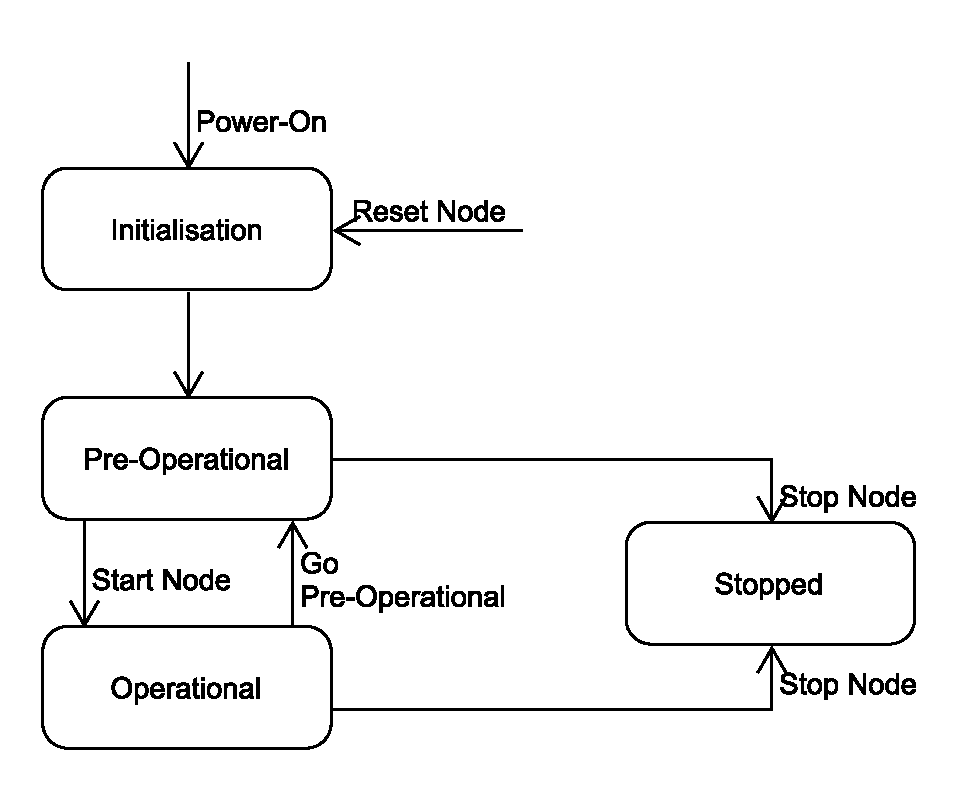
\includegraphics[width=10cm]{fsm_diagram}
\doxyfigcaption{F\+SM diagram}
\end{DoxyImage}
 
\chapter{Module Index}
\section{Modules}
Here is a list of all modules\+:\begin{DoxyCompactList}
\item \contentsline{section}{C\+AN Servizi Network}{\pageref{group___c_a_n__network__module}}{}
\begin{DoxyCompactList}
\item \contentsline{section}{C\+AN Network Nodes ID}{\pageref{group___c_a_n___i_d}}{}
\item \contentsline{section}{C\+A\+Nopen Function Codes}{\pageref{group___c_a_nopen___func___codes}}{}
\item \contentsline{section}{C\+A\+Nopen N\+MT module}{\pageref{group___c_a_nopen___n_m_t__group}}{}
\begin{DoxyCompactList}
\item \contentsline{section}{C\+A\+Nopen N\+MT Command Specifiers}{\pageref{group___c_a_nopen___n_m_t__speficications}}{}
\end{DoxyCompactList}
\item \contentsline{section}{C\+A\+Nopen P\+DO module}{\pageref{group___c_a_nopen___p_d_o__module}}{}
\item \contentsline{section}{C\+A\+Nopen Finite State Machine module}{\pageref{group___c_a_nopen___f_s_m__module}}{}
\item \contentsline{section}{C\+A\+Nopen Timer module}{\pageref{group___c_a_nopen__timer__module}}{}
\end{DoxyCompactList}
\item \contentsline{section}{Common Defines}{\pageref{group___common__defines__group}}{}
\begin{DoxyCompactList}
\item \contentsline{section}{S\+CU firmware selection}{\pageref{group___s_c_u__firmware__selection}}{}
\end{DoxyCompactList}
\item \contentsline{section}{Board module}{\pageref{group___board__model__group}}{}
\begin{DoxyCompactList}
\item \contentsline{section}{Data filtering module}{\pageref{group___filter__module__group}}{}
\item \contentsline{section}{Board pinout}{\pageref{group___board__pinout__group}}{}
\end{DoxyCompactList}
\item \contentsline{section}{Radio module}{\pageref{group___radio__module}}{}
\item \contentsline{section}{Main module}{\pageref{group___main__group__module}}{}
\end{DoxyCompactList}

\chapter{Class Index}
\section{Class List}
Here are the classes, structs, unions and interfaces with brief descriptions\+:\begin{DoxyCompactList}
\item\contentsline{section}{\mbox{\hyperlink{struct_message}{Message}} \\*C\+A\+Nopen message struct }{\pageref{struct_message}}{}
\end{DoxyCompactList}

\chapter{File Index}
\section{File List}
Here is a list of all documented files with brief descriptions\+:\begin{DoxyCompactList}
\item\contentsline{section}{\mbox{\hyperlink{_c_a_n___i_d_8h}{C\+A\+N\+\_\+\+I\+D.\+h}} \\*C\+AN servizi node\+I\+Ds module header }{\pageref{_c_a_n___i_d_8h}}{}
\item\contentsline{section}{\mbox{\hyperlink{_c_o__can_8cpp}{C\+O\+\_\+can.\+cpp}} \\*C\+A\+N\+Open main module implementation file }{\pageref{_c_o__can_8cpp}}{}
\item\contentsline{section}{\mbox{\hyperlink{_c_o__can_8h}{C\+O\+\_\+can.\+h}} \\*C\+A\+N\+Open main module header }{\pageref{_c_o__can_8h}}{}
\item\contentsline{section}{\mbox{\hyperlink{common_8h}{common.\+h}} \\*This file contains some common macro definitions for configuring main relevants parameters }{\pageref{common_8h}}{}
\item\contentsline{section}{\mbox{\hyperlink{def_8h}{def.\+h}} \\*C\+A\+Nopen D\+S301 definitions }{\pageref{def_8h}}{}
\item\contentsline{section}{\mbox{\hyperlink{filter_8cpp}{filter.\+cpp}} \\*Filter module implementation file }{\pageref{filter_8cpp}}{}
\item\contentsline{section}{\mbox{\hyperlink{filter_8h}{filter.\+h}} \\*Filter module header file }{\pageref{filter_8h}}{}
\item\contentsline{section}{\mbox{\hyperlink{model_8cpp}{model.\+cpp}} \\*Board model implementation file }{\pageref{model_8cpp}}{}
\item\contentsline{section}{\mbox{\hyperlink{model_8h}{model.\+h}} \\*Board model header file }{\pageref{model_8h}}{}
\item\contentsline{section}{\mbox{\hyperlink{nmt_8cpp}{nmt.\+cpp}} \\*C\+A\+N\+Open N\+MT module implementation file }{\pageref{nmt_8cpp}}{}
\item\contentsline{section}{\mbox{\hyperlink{nmt_8h}{nmt.\+h}} \\*C\+A\+N\+Open N\+MT module header }{\pageref{nmt_8h}}{}
\item\contentsline{section}{\mbox{\hyperlink{pdo_8cpp}{pdo.\+cpp}} \\*C\+A\+Nopen P\+DO support header file }{\pageref{pdo_8cpp}}{}
\item\contentsline{section}{\mbox{\hyperlink{pdo_8h}{pdo.\+h}} \\*C\+A\+Nopen P\+DO support header file }{\pageref{pdo_8h}}{}
\item\contentsline{section}{\mbox{\hyperlink{radio_8cpp}{radio.\+cpp}} \\*Radio implementation file }{\pageref{radio_8cpp}}{}
\item\contentsline{section}{\mbox{\hyperlink{radio_8h}{radio.\+h}} \\*Radio header file }{\pageref{radio_8h}}{}
\item\contentsline{section}{\mbox{\hyperlink{_s_c_u_8ino}{S\+C\+U.\+ino}} \\*Main module file }{\pageref{_s_c_u_8ino}}{}
\item\contentsline{section}{\mbox{\hyperlink{sensors__pinout_8h}{sensors\+\_\+pinout.\+h}} \\*Board pinout module header }{\pageref{sensors__pinout_8h}}{}
\item\contentsline{section}{\mbox{\hyperlink{states_8cpp}{states.\+cpp}} \\*C\+A\+Nopen finite state machine implementation file }{\pageref{states_8cpp}}{}
\item\contentsline{section}{\mbox{\hyperlink{states_8h}{states.\+h}} \\*C\+A\+Nopen finite state machine header file }{\pageref{states_8h}}{}
\item\contentsline{section}{\mbox{\hyperlink{timer_8cpp}{timer.\+cpp}} \\*C\+A\+Nopen timer implementation file }{\pageref{timer_8cpp}}{}
\item\contentsline{section}{\mbox{\hyperlink{timer_8h}{timer.\+h}} \\*C\+A\+Nopen timer header file }{\pageref{timer_8h}}{}
\end{DoxyCompactList}

\chapter{Module Documentation}
\hypertarget{group___c_a_n__network__module}{}\section{C\+AN Servizi Network}
\label{group___c_a_n__network__module}\index{C\+A\+N Servizi Network@{C\+A\+N Servizi Network}}
Collaboration diagram for C\+AN Servizi Network\+:\nopagebreak
\begin{figure}[H]
\begin{center}
\leavevmode
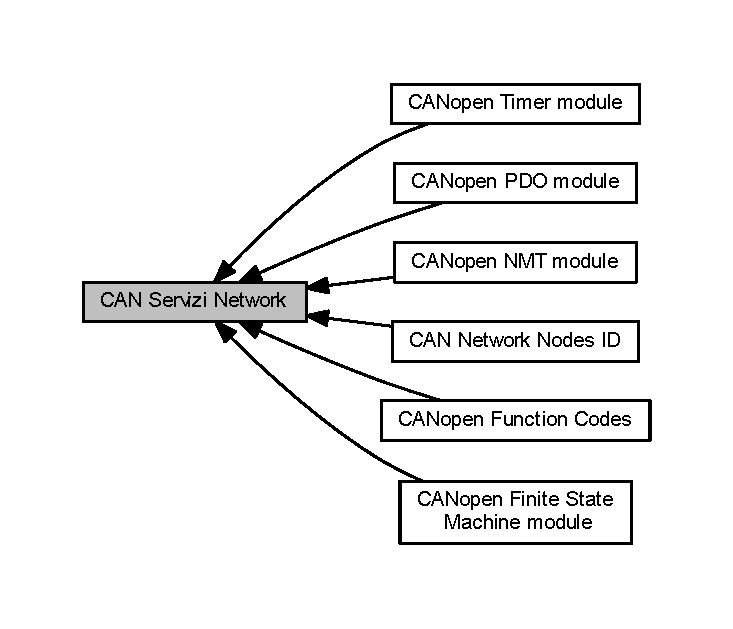
\includegraphics[width=350pt]{group___c_a_n__network__module}
\end{center}
\end{figure}
\subsection*{Modules}
\begin{DoxyCompactItemize}
\item 
\mbox{\hyperlink{group___c_a_n___i_d}{C\+A\+N Network Nodes ID}}
\item 
\mbox{\hyperlink{group___c_a_nopen___func___codes}{C\+A\+Nopen Function Codes}}
\item 
\mbox{\hyperlink{group___c_a_nopen___n_m_t__group}{C\+A\+Nopen N\+M\+T module}}
\item 
\mbox{\hyperlink{group___c_a_nopen___p_d_o__module}{C\+A\+Nopen P\+D\+O module}}
\end{DoxyCompactItemize}
\subsection*{Classes}
\begin{DoxyCompactItemize}
\item 
struct \mbox{\hyperlink{struct_message}{Message}}
\begin{DoxyCompactList}\small\item\em C\+A\+Nopen message struct. \end{DoxyCompactList}\end{DoxyCompactItemize}
\subsection*{Macros}
\begin{DoxyCompactItemize}
\item 
\mbox{\Hypertarget{group___c_a_n__network__module_gaf21e24a8e9f1bf113b5efb16d5ab924b}\label{group___c_a_n__network__module_gaf21e24a8e9f1bf113b5efb16d5ab924b}} 
\#define \mbox{\hyperlink{group___c_a_n__network__module_gaf21e24a8e9f1bf113b5efb16d5ab924b}{Message\+\_\+\+Initializer}}~\{0,0,\{0,0,0,0,0,0,0,0\}\}
\begin{DoxyCompactList}\small\item\em C\+A\+Nopen static message initializer. \end{DoxyCompactList}\end{DoxyCompactItemize}
\subsection*{Functions}
\begin{DoxyCompactItemize}
\item 
void \mbox{\hyperlink{group___c_a_n__network__module_ga44cc9b79c50c2c8eef6b98bac0d24dc9}{can\+Send}} (\mbox{\hyperlink{struct_message}{Message}} $\ast$m)
\begin{DoxyCompactList}\small\item\em This function send a C\+A\+Nopen message over C\+AN servizi network. \end{DoxyCompactList}\item 
\mbox{\Hypertarget{group___c_a_n__network__module_ga1b1534e44c5652543946053ad1aea5d1}\label{group___c_a_n__network__module_ga1b1534e44c5652543946053ad1aea5d1}} 
void {\bfseries C\+A\+N\+\_\+general\+\_\+callback} (C\+A\+N\+\_\+\+F\+R\+A\+ME $\ast$frame)
\item 
void \mbox{\hyperlink{group___c_a_n__network__module_gaee4f95b5d4a9e9c330f3a9169464860a}{init\+C\+AN}} ()
\begin{DoxyCompactList}\small\item\em This function initialize C\+A\+N/\+C\+A\+Nopen interfaces and communication. \end{DoxyCompactList}\end{DoxyCompactItemize}


\subsection{Detailed Description}


\subsection{Function Documentation}
\mbox{\Hypertarget{group___c_a_n__network__module_ga44cc9b79c50c2c8eef6b98bac0d24dc9}\label{group___c_a_n__network__module_ga44cc9b79c50c2c8eef6b98bac0d24dc9}} 
\index{C\+A\+N Servizi Network@{C\+A\+N Servizi Network}!can\+Send@{can\+Send}}
\index{can\+Send@{can\+Send}!C\+A\+N Servizi Network@{C\+A\+N Servizi Network}}
\subsubsection{\texorpdfstring{can\+Send()}{canSend()}}
{\footnotesize\ttfamily void can\+Send (\begin{DoxyParamCaption}\item[{\mbox{\hyperlink{struct_message}{Message}} $\ast$}]{m }\end{DoxyParamCaption})}



This function send a C\+A\+Nopen message over C\+AN servizi network. 

\begin{DoxyAuthor}{Author}
Arella Matteo ~\newline
 (mail\+: \href{mailto:arella.1646983@studenti.uniroma1.it}{\tt arella.\+1646983@studenti.\+uniroma1.\+it})
\end{DoxyAuthor}

\begin{DoxyParams}[1]{Parameters}
\mbox{\tt in}  & {\em m} & C\+A\+Nopen message to send \\
\hline
\end{DoxyParams}


Definition at line 20 of file C\+O\+\_\+can.\+cpp.

\mbox{\Hypertarget{group___c_a_n__network__module_gaee4f95b5d4a9e9c330f3a9169464860a}\label{group___c_a_n__network__module_gaee4f95b5d4a9e9c330f3a9169464860a}} 
\index{C\+A\+N Servizi Network@{C\+A\+N Servizi Network}!init\+C\+AN@{init\+C\+AN}}
\index{init\+C\+AN@{init\+C\+AN}!C\+A\+N Servizi Network@{C\+A\+N Servizi Network}}
\subsubsection{\texorpdfstring{init\+C\+A\+N()}{initCAN()}}
{\footnotesize\ttfamily void init\+C\+AN (\begin{DoxyParamCaption}{ }\end{DoxyParamCaption})}



This function initialize C\+A\+N/\+C\+A\+Nopen interfaces and communication. 

\begin{DoxyAuthor}{Author}
Arella Matteo ~\newline
 (mail\+: \href{mailto:arella.1646983@studenti.uniroma1.it}{\tt arella.\+1646983@studenti.\+uniroma1.\+it}) 
\end{DoxyAuthor}


Definition at line 42 of file C\+O\+\_\+can.\+cpp.


\hypertarget{group___c_a_n___i_d}{}\section{C\+AN Network Nodes ID}
\label{group___c_a_n___i_d}\index{C\+A\+N Network Nodes ID@{C\+A\+N Network Nodes ID}}
Collaboration diagram for C\+AN Network Nodes ID\+:\nopagebreak
\begin{figure}[H]
\begin{center}
\leavevmode
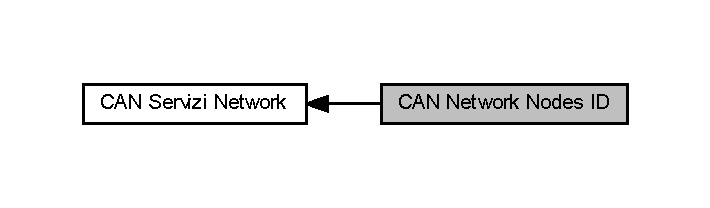
\includegraphics[width=341pt]{group___c_a_n___i_d}
\end{center}
\end{figure}
\subsection*{Macros}
\begin{DoxyCompactItemize}
\item 
\mbox{\Hypertarget{group___c_a_n___i_d_ga8d64b6b4c0f02ebded5440c6250e03b9}\label{group___c_a_n___i_d_ga8d64b6b4c0f02ebded5440c6250e03b9}} 
\#define \mbox{\hyperlink{group___c_a_n___i_d_ga8d64b6b4c0f02ebded5440c6250e03b9}{S\+C\+U\+\_\+\+F\+R\+O\+N\+T\+A\+L\+\_\+\+N\+O\+D\+E\+\_\+\+ID}}~1
\begin{DoxyCompactList}\small\item\em Frontal S\+CU node ID on C\+AN servizi network. \end{DoxyCompactList}\item 
\mbox{\Hypertarget{group___c_a_n___i_d_ga5703fd8de5ab8d0dcedb561f2178829e}\label{group___c_a_n___i_d_ga5703fd8de5ab8d0dcedb561f2178829e}} 
\#define \mbox{\hyperlink{group___c_a_n___i_d_ga5703fd8de5ab8d0dcedb561f2178829e}{V\+C\+U\+\_\+\+N\+O\+D\+E\+\_\+\+ID}}~2
\begin{DoxyCompactList}\small\item\em V\+CU node ID on C\+AN servizi network. \end{DoxyCompactList}\item 
\mbox{\Hypertarget{group___c_a_n___i_d_gab91968b64bc7fa886f6a6147d25d488b}\label{group___c_a_n___i_d_gab91968b64bc7fa886f6a6147d25d488b}} 
\#define \mbox{\hyperlink{group___c_a_n___i_d_gab91968b64bc7fa886f6a6147d25d488b}{S\+C\+U\+\_\+\+R\+E\+A\+R\+\_\+\+N\+O\+D\+E\+\_\+\+ID}}~3
\begin{DoxyCompactList}\small\item\em Rear S\+CU node ID on C\+AN servizi network. \end{DoxyCompactList}\item 
\mbox{\Hypertarget{group___c_a_n___i_d_gaceef3f7366b39e88d89cb98ad8094c7b}\label{group___c_a_n___i_d_gaceef3f7366b39e88d89cb98ad8094c7b}} 
\#define \mbox{\hyperlink{group___c_a_n___i_d_gaceef3f7366b39e88d89cb98ad8094c7b}{T\+C\+U\+\_\+\+N\+O\+D\+E\+\_\+\+ID}}~4
\begin{DoxyCompactList}\small\item\em T\+CU node ID on C\+AN servizi network. \end{DoxyCompactList}\end{DoxyCompactItemize}


\subsection{Detailed Description}

\hypertarget{group___common__defines__group}{}\section{Common Defines}
\label{group___common__defines__group}\index{Common Defines@{Common Defines}}
Collaboration diagram for Common Defines\+:\nopagebreak
\begin{figure}[H]
\begin{center}
\leavevmode
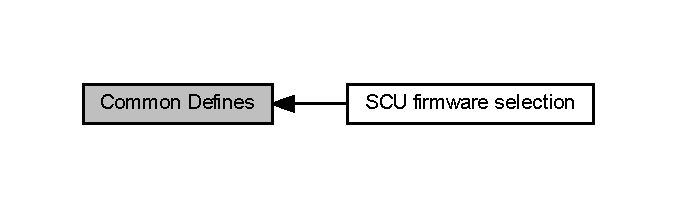
\includegraphics[width=325pt]{group___common__defines__group}
\end{center}
\end{figure}
\subsection*{Modules}
\begin{DoxyCompactItemize}
\item 
\mbox{\hyperlink{group___s_c_u__firmware__selection}{S\+C\+U firmware selection}}
\end{DoxyCompactItemize}
\subsection*{Macros}
\begin{DoxyCompactItemize}
\item 
\mbox{\Hypertarget{group___common__defines__group_gaa75b7ce1cd135619656735399baf3768}\label{group___common__defines__group_gaa75b7ce1cd135619656735399baf3768}} 
\#define \mbox{\hyperlink{group___common__defines__group_gaa75b7ce1cd135619656735399baf3768}{C\+A\+N\+\_\+\+B\+A\+U\+D\+R\+A\+TE}}~1000000
\begin{DoxyCompactList}\small\item\em C\+AN network baud rate \mbox{[} $bps$\mbox{]}. \end{DoxyCompactList}\item 
\mbox{\Hypertarget{group___common__defines__group_ga89f82a9d44beaa52b00c7245a50a105c}\label{group___common__defines__group_ga89f82a9d44beaa52b00c7245a50a105c}} 
\#define \mbox{\hyperlink{group___common__defines__group_ga89f82a9d44beaa52b00c7245a50a105c}{S\+E\+R\+I\+A\+L\+\_\+\+B\+A\+U\+D\+R\+A\+TE}}~115200
\begin{DoxyCompactList}\small\item\em Serial U\+A\+RT baud rate \mbox{[} $bps$\mbox{]}. \end{DoxyCompactList}\item 
\mbox{\Hypertarget{group___common__defines__group_ga09c95853fd002fab968d94c5bc44e823}\label{group___common__defines__group_ga09c95853fd002fab968d94c5bc44e823}} 
\#define \mbox{\hyperlink{group___common__defines__group_ga09c95853fd002fab968d94c5bc44e823}{T\+I\+M\+E\+\_\+\+S\+L\+O\+T\+\_\+\+P\+E\+R\+I\+OD}}~4000
\begin{DoxyCompactList}\small\item\em Timer period \mbox{[} $ms$\mbox{]}. \end{DoxyCompactList}\item 
\mbox{\Hypertarget{group___common__defines__group_ga599217205dc3092c26567a2bd868ef3a}\label{group___common__defines__group_ga599217205dc3092c26567a2bd868ef3a}} 
\#define \mbox{\hyperlink{group___common__defines__group_ga599217205dc3092c26567a2bd868ef3a}{T\+I\+M\+ER}}~Timer3
\begin{DoxyCompactList}\small\item\em C\+A\+Nopen timer. \end{DoxyCompactList}\end{DoxyCompactItemize}


\subsection{Detailed Description}

\hypertarget{group___s_c_u__firmware__selection}{}\section{S\+CU firmware selection}
\label{group___s_c_u__firmware__selection}\index{S\+C\+U firmware selection@{S\+C\+U firmware selection}}
Collaboration diagram for S\+CU firmware selection\+:\nopagebreak
\begin{figure}[H]
\begin{center}
\leavevmode
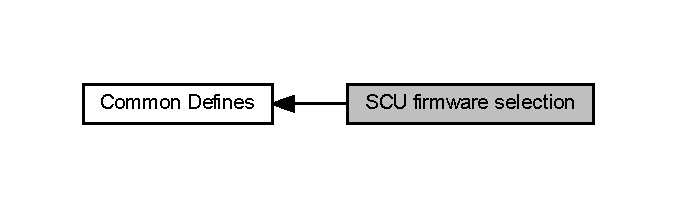
\includegraphics[width=325pt]{group___s_c_u__firmware__selection}
\end{center}
\end{figure}
\subsection*{Macros}
\begin{DoxyCompactItemize}
\item 
\mbox{\Hypertarget{group___s_c_u__firmware__selection_gac03ca83c43ea664674af7e07a8da7879}\label{group___s_c_u__firmware__selection_gac03ca83c43ea664674af7e07a8da7879}} 
\#define \mbox{\hyperlink{group___s_c_u__firmware__selection_gac03ca83c43ea664674af7e07a8da7879}{\+\_\+\+F\+R\+O\+N\+T\+A\+L\+\_\+}}
\begin{DoxyCompactList}\small\item\em Macro for selecting frontal S\+CU firmware. \end{DoxyCompactList}\item 
\mbox{\Hypertarget{group___s_c_u__firmware__selection_ga790010e78c29a0a2ffa3c09cc62d9f3d}\label{group___s_c_u__firmware__selection_ga790010e78c29a0a2ffa3c09cc62d9f3d}} 
\#define \mbox{\hyperlink{group___s_c_u__firmware__selection_ga790010e78c29a0a2ffa3c09cc62d9f3d}{\+\_\+\+R\+E\+T\+R\+O\+\_\+}}
\begin{DoxyCompactList}\small\item\em Macro for selecting rear S\+CU firmware. \end{DoxyCompactList}\end{DoxyCompactItemize}


\subsection{Detailed Description}
The firmware for each node is selectable during the precompilation of the code from the directives present in that module. Comment/uncomment those macros for active/deactive selected S\+CU firmware. 
\hypertarget{group___c_a_nopen___func___codes}{}\section{C\+A\+Nopen Function Codes}
\label{group___c_a_nopen___func___codes}\index{C\+A\+Nopen Function Codes@{C\+A\+Nopen Function Codes}}
Collaboration diagram for C\+A\+Nopen Function Codes\+:\nopagebreak
\begin{figure}[H]
\begin{center}
\leavevmode
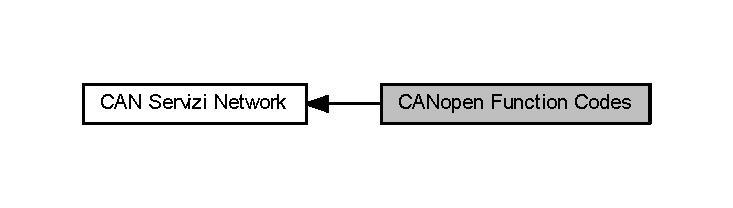
\includegraphics[width=350pt]{group___c_a_nopen___func___codes}
\end{center}
\end{figure}
\subsection*{Macros}
\begin{DoxyCompactItemize}
\item 
\mbox{\Hypertarget{group___c_a_nopen___func___codes_gaadbe0bb038acafa1c8adb0f98c870233}\label{group___c_a_nopen___func___codes_gaadbe0bb038acafa1c8adb0f98c870233}} 
\#define \mbox{\hyperlink{group___c_a_nopen___func___codes_gaadbe0bb038acafa1c8adb0f98c870233}{N\+MT}}~0x0
\begin{DoxyCompactList}\small\item\em N\+MT function code. \end{DoxyCompactList}\item 
\mbox{\Hypertarget{group___c_a_nopen___func___codes_ga9ac82e856c7683e23553431e5224d5f4}\label{group___c_a_nopen___func___codes_ga9ac82e856c7683e23553431e5224d5f4}} 
\#define \mbox{\hyperlink{group___c_a_nopen___func___codes_ga9ac82e856c7683e23553431e5224d5f4}{S\+Y\+NC}}~0x1
\begin{DoxyCompactList}\small\item\em S\+Y\+NC function code. \end{DoxyCompactList}\item 
\mbox{\Hypertarget{group___c_a_nopen___func___codes_ga5a63bf5566f66e30f56bc17eea0e5e4b}\label{group___c_a_nopen___func___codes_ga5a63bf5566f66e30f56bc17eea0e5e4b}} 
\#define \mbox{\hyperlink{group___c_a_nopen___func___codes_ga5a63bf5566f66e30f56bc17eea0e5e4b}{T\+I\+M\+E\+\_\+\+S\+T\+A\+MP}}~0x2
\begin{DoxyCompactList}\small\item\em T\+I\+M\+E\+\_\+\+S\+T\+A\+MP function code. \end{DoxyCompactList}\item 
\mbox{\Hypertarget{group___c_a_nopen___func___codes_ga0a250614ba4dca3e87f768efcb58f238}\label{group___c_a_nopen___func___codes_ga0a250614ba4dca3e87f768efcb58f238}} 
\#define \mbox{\hyperlink{group___c_a_nopen___func___codes_ga0a250614ba4dca3e87f768efcb58f238}{P\+D\+O1tx}}~0x3
\begin{DoxyCompactList}\small\item\em P\+D\+O1tx function code. \end{DoxyCompactList}\item 
\mbox{\Hypertarget{group___c_a_nopen___func___codes_ga17c7ee302d491b1ef74d2a4a795f82c6}\label{group___c_a_nopen___func___codes_ga17c7ee302d491b1ef74d2a4a795f82c6}} 
\#define \mbox{\hyperlink{group___c_a_nopen___func___codes_ga17c7ee302d491b1ef74d2a4a795f82c6}{P\+D\+O1rx}}~0x4
\begin{DoxyCompactList}\small\item\em P\+D\+O1rx function code. \end{DoxyCompactList}\item 
\mbox{\Hypertarget{group___c_a_nopen___func___codes_ga67f4224b2c072a82b37a4835ca1c75e1}\label{group___c_a_nopen___func___codes_ga67f4224b2c072a82b37a4835ca1c75e1}} 
\#define \mbox{\hyperlink{group___c_a_nopen___func___codes_ga67f4224b2c072a82b37a4835ca1c75e1}{P\+D\+O2tx}}~0x5
\begin{DoxyCompactList}\small\item\em P\+D\+O2tx function code. \end{DoxyCompactList}\item 
\mbox{\Hypertarget{group___c_a_nopen___func___codes_gab23848999420738438097816fee3f25d}\label{group___c_a_nopen___func___codes_gab23848999420738438097816fee3f25d}} 
\#define \mbox{\hyperlink{group___c_a_nopen___func___codes_gab23848999420738438097816fee3f25d}{P\+D\+O2rx}}~0x6
\begin{DoxyCompactList}\small\item\em P\+D\+O2rx function code. \end{DoxyCompactList}\item 
\mbox{\Hypertarget{group___c_a_nopen___func___codes_ga00ef0f6ae698f9cb944b4302e66e6c83}\label{group___c_a_nopen___func___codes_ga00ef0f6ae698f9cb944b4302e66e6c83}} 
\#define \mbox{\hyperlink{group___c_a_nopen___func___codes_ga00ef0f6ae698f9cb944b4302e66e6c83}{P\+D\+O3tx}}~0x7
\begin{DoxyCompactList}\small\item\em P\+D\+O3tx function code. \end{DoxyCompactList}\item 
\mbox{\Hypertarget{group___c_a_nopen___func___codes_ga239d135abea5ec798461cad43f9286b5}\label{group___c_a_nopen___func___codes_ga239d135abea5ec798461cad43f9286b5}} 
\#define \mbox{\hyperlink{group___c_a_nopen___func___codes_ga239d135abea5ec798461cad43f9286b5}{P\+D\+O3rx}}~0x8
\begin{DoxyCompactList}\small\item\em P\+D\+O3rx function code. \end{DoxyCompactList}\item 
\mbox{\Hypertarget{group___c_a_nopen___func___codes_gabda4cc9ec44d1fc524bfdcae030df4be}\label{group___c_a_nopen___func___codes_gabda4cc9ec44d1fc524bfdcae030df4be}} 
\#define \mbox{\hyperlink{group___c_a_nopen___func___codes_gabda4cc9ec44d1fc524bfdcae030df4be}{P\+D\+O4tx}}~0x9
\begin{DoxyCompactList}\small\item\em P\+D\+O4tx function code. \end{DoxyCompactList}\item 
\mbox{\Hypertarget{group___c_a_nopen___func___codes_ga282f714f745dd28e9a017044020aa3dc}\label{group___c_a_nopen___func___codes_ga282f714f745dd28e9a017044020aa3dc}} 
\#define \mbox{\hyperlink{group___c_a_nopen___func___codes_ga282f714f745dd28e9a017044020aa3dc}{P\+D\+O4rx}}~0xA
\begin{DoxyCompactList}\small\item\em P\+D\+O4rx function code. \end{DoxyCompactList}\item 
\mbox{\Hypertarget{group___c_a_nopen___func___codes_ga74331e9b1d102bd0a3d5d9c1fc4f8212}\label{group___c_a_nopen___func___codes_ga74331e9b1d102bd0a3d5d9c1fc4f8212}} 
\#define \mbox{\hyperlink{group___c_a_nopen___func___codes_ga74331e9b1d102bd0a3d5d9c1fc4f8212}{S\+D\+Otx}}~0xB
\begin{DoxyCompactList}\small\item\em S\+D\+Otx function code. \end{DoxyCompactList}\item 
\mbox{\Hypertarget{group___c_a_nopen___func___codes_ga44318f0cf5176db0eedd1c8519bd8f35}\label{group___c_a_nopen___func___codes_ga44318f0cf5176db0eedd1c8519bd8f35}} 
\#define \mbox{\hyperlink{group___c_a_nopen___func___codes_ga44318f0cf5176db0eedd1c8519bd8f35}{S\+D\+Orx}}~0xC
\begin{DoxyCompactList}\small\item\em S\+D\+Orx function code. \end{DoxyCompactList}\item 
\mbox{\Hypertarget{group___c_a_nopen___func___codes_ga78d5d3f71db9f360c9e3d3953707b0c1}\label{group___c_a_nopen___func___codes_ga78d5d3f71db9f360c9e3d3953707b0c1}} 
\#define \mbox{\hyperlink{group___c_a_nopen___func___codes_ga78d5d3f71db9f360c9e3d3953707b0c1}{N\+O\+D\+E\+\_\+\+G\+U\+A\+RD}}~0xE
\begin{DoxyCompactList}\small\item\em N\+O\+DE G\+U\+A\+RD function code. \end{DoxyCompactList}\item 
\mbox{\Hypertarget{group___c_a_nopen___func___codes_gaa09b700d4c6a1eac2a3068f446c397e2}\label{group___c_a_nopen___func___codes_gaa09b700d4c6a1eac2a3068f446c397e2}} 
\#define \mbox{\hyperlink{group___c_a_nopen___func___codes_gaa09b700d4c6a1eac2a3068f446c397e2}{L\+SS}}~0xF
\begin{DoxyCompactList}\small\item\em L\+SS function code. \end{DoxyCompactList}\item 
\mbox{\Hypertarget{group___c_a_nopen___func___codes_gad4585eb139cc908014093ce9b81d0d51}\label{group___c_a_nopen___func___codes_gad4585eb139cc908014093ce9b81d0d51}} 
\#define \mbox{\hyperlink{group___c_a_nopen___func___codes_gad4585eb139cc908014093ce9b81d0d51}{G\+E\+T\+\_\+\+F\+U\+N\+C\+\_\+\+C\+O\+DE}}(C\+O\+B\+\_\+\+ID)~(C\+O\+B\+\_\+\+ID $>$$>$ 7)
\begin{DoxyCompactList}\small\item\em Extract function code from C\+O\+B-\/\+ID. \end{DoxyCompactList}\item 
\mbox{\Hypertarget{group___c_a_nopen___func___codes_gade75ae84ef68190e83a60643194e91fd}\label{group___c_a_nopen___func___codes_gade75ae84ef68190e83a60643194e91fd}} 
\#define \mbox{\hyperlink{group___c_a_nopen___func___codes_gade75ae84ef68190e83a60643194e91fd}{S\+E\+T\+\_\+\+F\+U\+N\+C\+\_\+\+C\+O\+DE}}(C\+O\+B\+\_\+\+ID)~(C\+O\+B\+\_\+\+ID $<$$<$ 7)
\begin{DoxyCompactList}\small\item\em Set function code to C\+O\+B-\/\+ID. \end{DoxyCompactList}\end{DoxyCompactItemize}


\subsection{Detailed Description}
C\+A\+Nopen function codes defined in D\+S301 profile. 
\hypertarget{group___c_a_nopen___n_m_t__speficications}{}\section{C\+A\+Nopen N\+MT Command Specifiers}
\label{group___c_a_nopen___n_m_t__speficications}\index{C\+A\+Nopen N\+M\+T Command Specifiers@{C\+A\+Nopen N\+M\+T Command Specifiers}}
Collaboration diagram for C\+A\+Nopen N\+MT Command Specifiers\+:\nopagebreak
\begin{figure}[H]
\begin{center}
\leavevmode
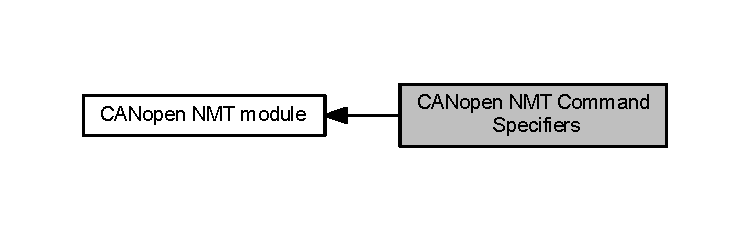
\includegraphics[width=350pt]{group___c_a_nopen___n_m_t__speficications}
\end{center}
\end{figure}
\subsection*{Macros}
\begin{DoxyCompactItemize}
\item 
\mbox{\Hypertarget{group___c_a_nopen___n_m_t__speficications_ga9654207fdc32413aa792c8a2dc9d414f}\label{group___c_a_nopen___n_m_t__speficications_ga9654207fdc32413aa792c8a2dc9d414f}} 
\#define \mbox{\hyperlink{group___c_a_nopen___n_m_t__speficications_ga9654207fdc32413aa792c8a2dc9d414f}{N\+M\+T\+\_\+\+Start\+\_\+\+Node}}~0x01
\begin{DoxyCompactList}\small\item\em \textquotesingle{}go Operational\textquotesingle{} command specifier \end{DoxyCompactList}\item 
\mbox{\Hypertarget{group___c_a_nopen___n_m_t__speficications_ga7aae99c67e9ebd9491a246baf92570fa}\label{group___c_a_nopen___n_m_t__speficications_ga7aae99c67e9ebd9491a246baf92570fa}} 
\#define \mbox{\hyperlink{group___c_a_nopen___n_m_t__speficications_ga7aae99c67e9ebd9491a246baf92570fa}{N\+M\+T\+\_\+\+Stop\+\_\+\+Node}}~0x02
\begin{DoxyCompactList}\small\item\em \textquotesingle{}stop Node\textquotesingle{} command specifier \end{DoxyCompactList}\item 
\mbox{\Hypertarget{group___c_a_nopen___n_m_t__speficications_gabdbbb7ecbe41058f60f684c10e07e08e}\label{group___c_a_nopen___n_m_t__speficications_gabdbbb7ecbe41058f60f684c10e07e08e}} 
\#define \mbox{\hyperlink{group___c_a_nopen___n_m_t__speficications_gabdbbb7ecbe41058f60f684c10e07e08e}{N\+M\+T\+\_\+\+Enter\+\_\+\+Pre\+Operational}}~0x80
\begin{DoxyCompactList}\small\item\em \textquotesingle{}go Pre\+Operational\textquotesingle{} command specifier \end{DoxyCompactList}\item 
\mbox{\Hypertarget{group___c_a_nopen___n_m_t__speficications_gab349b5574a1ea67ff0ef76b9f9b6319e}\label{group___c_a_nopen___n_m_t__speficications_gab349b5574a1ea67ff0ef76b9f9b6319e}} 
\#define \mbox{\hyperlink{group___c_a_nopen___n_m_t__speficications_gab349b5574a1ea67ff0ef76b9f9b6319e}{N\+M\+T\+\_\+\+Reset\+\_\+\+Node}}~0x81
\begin{DoxyCompactList}\small\item\em \textquotesingle{}reset Node\textquotesingle{} command specifier \end{DoxyCompactList}\item 
\mbox{\Hypertarget{group___c_a_nopen___n_m_t__speficications_gafd16bdbe636d7c761a9e015a7d7653ce}\label{group___c_a_nopen___n_m_t__speficications_gafd16bdbe636d7c761a9e015a7d7653ce}} 
\#define \mbox{\hyperlink{group___c_a_nopen___n_m_t__speficications_gafd16bdbe636d7c761a9e015a7d7653ce}{N\+M\+T\+\_\+\+Reset\+\_\+\+Comunication}}~0x82
\begin{DoxyCompactList}\small\item\em \textquotesingle{}reset Communication\textquotesingle{} command specifier \end{DoxyCompactList}\end{DoxyCompactItemize}


\subsection{Detailed Description}

\hypertarget{group___filter__module__group}{}\section{Data filtering module}
\label{group___filter__module__group}\index{Data filtering module@{Data filtering module}}
Collaboration diagram for Data filtering module\+:\nopagebreak
\begin{figure}[H]
\begin{center}
\leavevmode
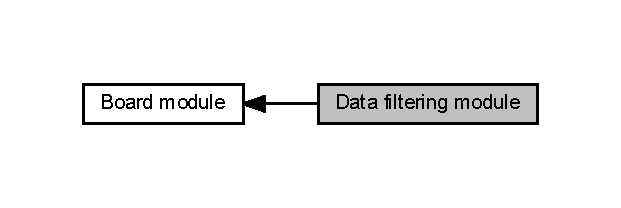
\includegraphics[width=298pt]{group___filter__module__group}
\end{center}
\end{figure}
\subsection*{Macros}
\begin{DoxyCompactItemize}
\item 
\mbox{\Hypertarget{group___filter__module__group_ga1646c21a91b653eeb516c9d508c1cab6}\label{group___filter__module__group_ga1646c21a91b653eeb516c9d508c1cab6}} 
\#define \mbox{\hyperlink{group___filter__module__group_ga1646c21a91b653eeb516c9d508c1cab6}{U\+S\+E\+\_\+\+L\+O\+O\+P\+\_\+\+U\+N\+R\+O\+L\+L\+I\+NG}}~(1)
\begin{DoxyCompactList}\small\item\em Flag macro for using or not loop unrolling into filter function. \end{DoxyCompactList}\item 
\mbox{\Hypertarget{group___filter__module__group_gaa505bfa61df2c48cb76be56720dae3d1}\label{group___filter__module__group_gaa505bfa61df2c48cb76be56720dae3d1}} 
\#define \mbox{\hyperlink{group___filter__module__group_gaa505bfa61df2c48cb76be56720dae3d1}{pos}}(x,  offset)~((x) $\ast$ offset)
\begin{DoxyCompactList}\small\item\em Buffer indexing macro. \end{DoxyCompactList}\end{DoxyCompactItemize}
\subsection*{Functions}
\begin{DoxyCompactItemize}
\item 
uint16\+\_\+t \mbox{\hyperlink{group___filter__module__group_ga676952eee893902e5a15b3f5adca1f86}{filter\+\_\+buffer}} (volatile uint16\+\_\+t $\ast$buffer, int size, unsigned offset)
\begin{DoxyCompactList}\small\item\em This function filters the input buffer with an average filter. \end{DoxyCompactList}\end{DoxyCompactItemize}


\subsection{Detailed Description}


\subsection{Function Documentation}
\mbox{\Hypertarget{group___filter__module__group_ga676952eee893902e5a15b3f5adca1f86}\label{group___filter__module__group_ga676952eee893902e5a15b3f5adca1f86}} 
\index{Data filtering module@{Data filtering module}!filter\+\_\+buffer@{filter\+\_\+buffer}}
\index{filter\+\_\+buffer@{filter\+\_\+buffer}!Data filtering module@{Data filtering module}}
\subsubsection{\texorpdfstring{filter\+\_\+buffer()}{filter\_buffer()}}
{\footnotesize\ttfamily uint16\+\_\+t filter\+\_\+buffer (\begin{DoxyParamCaption}\item[{volatile uint16\+\_\+t $\ast$}]{buffer,  }\item[{int}]{size,  }\item[{unsigned}]{offset }\end{DoxyParamCaption})}



This function filters the input buffer with an average filter. 

\begin{DoxyAuthor}{Author}
Arella Matteo ~\newline
 (mail\+: \href{mailto:arella.1646983@studenti.uniroma1.it}{\tt arella.\+1646983@studenti.\+uniroma1.\+it})
\end{DoxyAuthor}

\begin{DoxyParams}[1]{Parameters}
\mbox{\tt in}  & {\em buffer} & Input buffer \\
\hline
\mbox{\tt in}  & {\em size} & Buffer size \\
\hline
\mbox{\tt in}  & {\em offset} & Offset between data corresponding to same acquired value \\
\hline
\end{DoxyParams}
\begin{DoxyReturn}{Returns}
Filtered data 
\end{DoxyReturn}


Definition at line 39 of file filter.\+cpp.


\hypertarget{group___board__model__group}{}\section{Board module}
\label{group___board__model__group}\index{Board module@{Board module}}
Collaboration diagram for Board module\+:\nopagebreak
\begin{figure}[H]
\begin{center}
\leavevmode
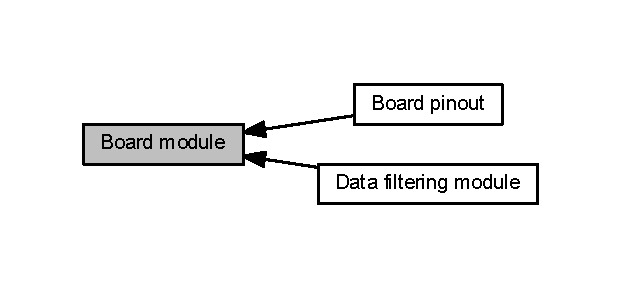
\includegraphics[width=298pt]{group___board__model__group}
\end{center}
\end{figure}
\subsection*{Modules}
\begin{DoxyCompactItemize}
\item 
\mbox{\hyperlink{group___filter__module__group}{Data filtering module}}
\item 
\mbox{\hyperlink{group___board__pinout__group}{Board pinout}}
\end{DoxyCompactItemize}
\subsection*{Macros}
\begin{DoxyCompactItemize}
\item 
\mbox{\Hypertarget{group___board__model__group_ga602abb8ec84dcb3b6f854a738310ea46}\label{group___board__model__group_ga602abb8ec84dcb3b6f854a738310ea46}} 
\#define \mbox{\hyperlink{group___board__model__group_ga602abb8ec84dcb3b6f854a738310ea46}{A\+D\+C\+\_\+\+B\+U\+F\+F\+E\+R\+\_\+\+S\+I\+ZE}}~128
\begin{DoxyCompactList}\small\item\em Size (bytes) of buffer for store each A\+DC channel data with D\+MA. \end{DoxyCompactList}\item 
\#define \mbox{\hyperlink{group___board__model__group_gaabe0f927d44a09f458bd5fe5ab4e2f7f}{B\+U\+F\+F\+E\+RS}}~4
\begin{DoxyCompactList}\small\item\em Number of D\+MA buffers. \end{DoxyCompactList}\item 
\mbox{\Hypertarget{group___board__model__group_gaf0098a1eafb8a60a1c65773e1064d595}\label{group___board__model__group_gaf0098a1eafb8a60a1c65773e1064d595}} 
\#define \mbox{\hyperlink{group___board__model__group_gaf0098a1eafb8a60a1c65773e1064d595}{A\+D\+C\+\_\+\+M\+IN}}~0
\begin{DoxyCompactList}\small\item\em A\+DC lower bound value. \end{DoxyCompactList}\item 
\mbox{\Hypertarget{group___board__model__group_ga555a695bf58df062dc03f0e892d95cd7}\label{group___board__model__group_ga555a695bf58df062dc03f0e892d95cd7}} 
\#define \mbox{\hyperlink{group___board__model__group_ga555a695bf58df062dc03f0e892d95cd7}{A\+D\+C\+\_\+\+M\+AX}}~4095
\begin{DoxyCompactList}\small\item\em A\+DC upper bound value. \end{DoxyCompactList}\item 
\mbox{\Hypertarget{group___board__model__group_ga6741cba3daf129b6f73eed1b1db09519}\label{group___board__model__group_ga6741cba3daf129b6f73eed1b1db09519}} 
\#define \mbox{\hyperlink{group___board__model__group_ga6741cba3daf129b6f73eed1b1db09519}{T\+P\+S1\+\_\+\+U\+P\+P\+E\+R\+\_\+\+B\+O\+U\+ND}}~2482
\begin{DoxyCompactList}\small\item\em First A\+P\+PS max output voltage (2V) \end{DoxyCompactList}\item 
\mbox{\Hypertarget{group___board__model__group_ga9c9aa914f6b372d9ef3f15ce4108da6a}\label{group___board__model__group_ga9c9aa914f6b372d9ef3f15ce4108da6a}} 
\#define \mbox{\hyperlink{group___board__model__group_ga9c9aa914f6b372d9ef3f15ce4108da6a}{T\+P\+S1\+\_\+\+L\+O\+W\+E\+R\+\_\+\+B\+O\+U\+ND}}~993
\begin{DoxyCompactList}\small\item\em First A\+P\+PS min output voltage (0.\+8V) \end{DoxyCompactList}\item 
\mbox{\Hypertarget{group___board__model__group_gac8be8d89c699c40b79d04c0fdf6238f4}\label{group___board__model__group_gac8be8d89c699c40b79d04c0fdf6238f4}} 
\#define \mbox{\hyperlink{group___board__model__group_gac8be8d89c699c40b79d04c0fdf6238f4}{T\+P\+S2\+\_\+\+U\+P\+P\+E\+R\+\_\+\+B\+O\+U\+ND}}~1241
\begin{DoxyCompactList}\small\item\em Second A\+P\+PS max output voltage (1V) \end{DoxyCompactList}\item 
\mbox{\Hypertarget{group___board__model__group_gadfcc723e175ac44e73e38407299ac875}\label{group___board__model__group_gadfcc723e175ac44e73e38407299ac875}} 
\#define \mbox{\hyperlink{group___board__model__group_gadfcc723e175ac44e73e38407299ac875}{T\+P\+S2\+\_\+\+L\+O\+W\+E\+R\+\_\+\+B\+O\+U\+ND}}~497
\begin{DoxyCompactList}\small\item\em Second A\+P\+PS min output voltage (0.\+4V) \end{DoxyCompactList}\item 
\mbox{\Hypertarget{group___board__model__group_ga891de03ab9e1bd9a92ffffe69a1b10ca}\label{group___board__model__group_ga891de03ab9e1bd9a92ffffe69a1b10ca}} 
\#define \mbox{\hyperlink{group___board__model__group_ga891de03ab9e1bd9a92ffffe69a1b10ca}{B\+R\+A\+K\+E\+\_\+\+U\+P\+P\+E\+R\+\_\+\+B\+O\+U\+ND}}~0
\begin{DoxyCompactList}\small\item\em Brake sensor max output voltage (T\+O\+DO\+: check Voutmax) \end{DoxyCompactList}\item 
\mbox{\Hypertarget{group___board__model__group_ga0aed20cafcc206360abda47b125432c7}\label{group___board__model__group_ga0aed20cafcc206360abda47b125432c7}} 
\#define \mbox{\hyperlink{group___board__model__group_ga0aed20cafcc206360abda47b125432c7}{B\+R\+A\+K\+E\+\_\+\+L\+O\+W\+E\+R\+\_\+\+B\+O\+U\+ND}}~\mbox{\hyperlink{group___board__model__group_ga555a695bf58df062dc03f0e892d95cd7}{A\+D\+C\+\_\+\+M\+AX}}
\begin{DoxyCompactList}\small\item\em Brake sensor min output voltage (T\+O\+DO\+: check Voutmin) \end{DoxyCompactList}\item 
\mbox{\Hypertarget{group___board__model__group_ga2445bb784c1bcde9b88c5f81fc814055}\label{group___board__model__group_ga2445bb784c1bcde9b88c5f81fc814055}} 
\#define \mbox{\hyperlink{group___board__model__group_ga2445bb784c1bcde9b88c5f81fc814055}{S\+U\+S\+P\+E\+N\+S\+I\+O\+N\+S\+\_\+\+M\+IN}}~0
\begin{DoxyCompactList}\small\item\em Minimum suspension stroke \mbox{[} $mm$\mbox{]}. \end{DoxyCompactList}\item 
\mbox{\Hypertarget{group___board__model__group_gaf662e0e156dae3a519648a2f10fa3635}\label{group___board__model__group_gaf662e0e156dae3a519648a2f10fa3635}} 
\#define \mbox{\hyperlink{group___board__model__group_gaf662e0e156dae3a519648a2f10fa3635}{S\+U\+S\+P\+E\+N\+S\+I\+O\+N\+S\+\_\+\+A\+D\+C\+\_\+\+M\+AX}}~\mbox{\hyperlink{group___board__model__group_ga555a695bf58df062dc03f0e892d95cd7}{A\+D\+C\+\_\+\+M\+AX}}
\begin{DoxyCompactList}\small\item\em Maximum suspension sensor $V_{OUT}$. \end{DoxyCompactList}\item 
\mbox{\Hypertarget{group___board__model__group_gadad409d745f70ca3c312ca3914a43822}\label{group___board__model__group_gadad409d745f70ca3c312ca3914a43822}} 
\#define \mbox{\hyperlink{group___board__model__group_gadad409d745f70ca3c312ca3914a43822}{S\+U\+S\+P\+\_\+\+S\+T\+R\+O\+K\+E\+\_\+\+N\+O\+R\+M\+A\+L\+I\+ZE}}~(\mbox{\hyperlink{group___board__model__group_gafd34b4e5a1067ffe9bfb1cb18b5973e6}{S\+U\+S\+P\+\_\+\+S\+T\+R\+O\+K\+E\+\_\+\+E\+X\+T\+E\+N\+S\+I\+ON}} / \mbox{\hyperlink{group___board__model__group_gaf662e0e156dae3a519648a2f10fa3635}{S\+U\+S\+P\+E\+N\+S\+I\+O\+N\+S\+\_\+\+A\+D\+C\+\_\+\+M\+AX}})
\begin{DoxyCompactList}\small\item\em Suspension stroke voltage normalizer. \end{DoxyCompactList}\item 
\mbox{\Hypertarget{group___board__model__group_gab4fd15d90627818134453e8399055f7d}\label{group___board__model__group_gab4fd15d90627818134453e8399055f7d}} 
\#define \mbox{\hyperlink{group___board__model__group_gab4fd15d90627818134453e8399055f7d}{C\+O\+G\+S\+\_\+\+N\+U\+M\+B\+ER}}~30.\+0d
\begin{DoxyCompactList}\small\item\em Number of phonic wheel\textquotesingle{}s cogs. \end{DoxyCompactList}\item 
\mbox{\Hypertarget{group___board__model__group_ga579e1065b83e6aef14ce222295f8b7eb}\label{group___board__model__group_ga579e1065b83e6aef14ce222295f8b7eb}} 
\#define \mbox{\hyperlink{group___board__model__group_ga579e1065b83e6aef14ce222295f8b7eb}{N\+O\+R\+M\+A\+L\+I\+Z\+E\+\_\+\+R\+PM}}~1000000.\+0d
\begin{DoxyCompactList}\small\item\em Normalize time domain \mbox{[} $\mu s$\mbox{]}. \end{DoxyCompactList}\item 
\mbox{\Hypertarget{group___board__model__group_gafc05771487f188ffa40b6620afc1a9bc}\label{group___board__model__group_gafc05771487f188ffa40b6620afc1a9bc}} 
\#define \mbox{\hyperlink{group___board__model__group_gafc05771487f188ffa40b6620afc1a9bc}{R\+P\+M\+\_\+\+M\+IN}}~10
\begin{DoxyCompactList}\small\item\em Rpm lower bound under that rpm are forced to zero. \end{DoxyCompactList}\item 
\mbox{\Hypertarget{group___board__model__group_gaa8634c7b040cfe3e016765395a38efa3}\label{group___board__model__group_gaa8634c7b040cfe3e016765395a38efa3}} 
\#define \mbox{\hyperlink{group___board__model__group_gaa8634c7b040cfe3e016765395a38efa3}{A\+C\+C\+E\+L\+E\+R\+O\+M\+E\+T\+E\+R\+\_\+\+M\+A\+X\+\_\+G}}~5.\+0d
\begin{DoxyCompactList}\small\item\em Accelerometer sensor maximum value \mbox{[} $m/s^{2}$\mbox{]}. \end{DoxyCompactList}\item 
\mbox{\Hypertarget{group___board__model__group_ga5b18e6cd4163d6006ddf3c1f8a1e2a72}\label{group___board__model__group_ga5b18e6cd4163d6006ddf3c1f8a1e2a72}} 
\#define \mbox{\hyperlink{group___board__model__group_ga5b18e6cd4163d6006ddf3c1f8a1e2a72}{A\+C\+C\+E\+L\+E\+R\+O\+M\+E\+T\+E\+R\+\_\+\+N\+O\+R\+M\+A\+L\+I\+ZE}}~2.\+0d $\ast$ A\+C\+C\+E\+L\+E\+R\+O\+M\+E\+T\+E\+R\+\_\+\+M\+A\+X\+\_\+\+G / A\+D\+C\+\_\+\+M\+AX
\begin{DoxyCompactList}\small\item\em Accelerometer sensor voltage normalizer. \end{DoxyCompactList}\item 
\mbox{\Hypertarget{group___board__model__group_ga3e1022cd2e2154437b583f7ff83f2960}\label{group___board__model__group_ga3e1022cd2e2154437b583f7ff83f2960}} 
\#define \mbox{\hyperlink{group___board__model__group_ga3e1022cd2e2154437b583f7ff83f2960}{A\+P\+P\+S\+\_\+\+P\+L\+A\+U\+S\+\_\+\+R\+A\+N\+GE}}~10
\begin{DoxyCompactList}\small\item\em Maximum percentage deviation of pedal travel between two A\+P\+PS. \end{DoxyCompactList}\item 
\mbox{\Hypertarget{group___board__model__group_ga99f732ac210a4d6b6635ed58681d3d71}\label{group___board__model__group_ga99f732ac210a4d6b6635ed58681d3d71}} 
\#define \mbox{\hyperlink{group___board__model__group_ga99f732ac210a4d6b6635ed58681d3d71}{S\+C\+U\+\_\+\+F\+R\+O\+N\+T\+A\+L\+\_\+\+A\+D\+C\+\_\+\+C\+H\+A\+N\+N\+E\+LS}}~5
\begin{DoxyCompactList}\small\item\em Number of A\+DC channels used in frontal S\+CU board. \end{DoxyCompactList}\item 
\mbox{\Hypertarget{group___board__model__group_ga1b36d02d5fef3342ea7159722fa50ff3}\label{group___board__model__group_ga1b36d02d5fef3342ea7159722fa50ff3}} 
\#define \mbox{\hyperlink{group___board__model__group_ga1b36d02d5fef3342ea7159722fa50ff3}{S\+C\+U\+\_\+\+F\+R\+O\+N\+T\+A\+L\+\_\+\+A\+D\+C\+\_\+\+C\+H\+A\+N\+N\+E\+L\+S\+\_\+\+L\+I\+ST}}~\mbox{\hyperlink{group___board__pinout__group_ga99b2a7dadaf495e3c559a46440f9141f}{T\+P\+S1\+\_\+\+A\+D\+C\+\_\+\+C\+H\+A\+N\+\_\+\+N\+UM}} $\vert$ \mbox{\hyperlink{group___board__pinout__group_ga4cecb8c10512873904099a1a88d69ed3}{T\+P\+S2\+\_\+\+A\+D\+C\+\_\+\+C\+H\+A\+N\+\_\+\+N\+UM}} $\vert$ \mbox{\hyperlink{group___board__pinout__group_ga310547321c4a016c4ad19922920fadfd}{B\+R\+A\+K\+E\+\_\+\+A\+D\+C\+\_\+\+C\+H\+A\+N\+\_\+\+N\+UM}} $\vert$ \mbox{\hyperlink{group___board__pinout__group_ga3582ac3b04abaa9d74b16da2b18a62f9}{F\+R\+\_\+\+S\+X\+\_\+\+S\+U\+S\+P\+\_\+\+A\+D\+C\+\_\+\+C\+H\+A\+N\+\_\+\+N\+UM}} $\vert$ \mbox{\hyperlink{group___board__pinout__group_ga0e9f0303c372af214367d86ad38f660d}{F\+R\+\_\+\+D\+X\+\_\+\+S\+U\+S\+P\+\_\+\+A\+D\+C\+\_\+\+C\+H\+A\+N\+\_\+\+N\+UM}}
\begin{DoxyCompactList}\small\item\em List of A\+DC channels dedicated to each IO port in frontal S\+CU board. \end{DoxyCompactList}\item 
\mbox{\Hypertarget{group___board__model__group_gadedc78ae5ed236e74a4e12c031209d29}\label{group___board__model__group_gadedc78ae5ed236e74a4e12c031209d29}} 
\#define \mbox{\hyperlink{group___board__model__group_gadedc78ae5ed236e74a4e12c031209d29}{S\+C\+U\+\_\+\+R\+E\+T\+R\+O\+\_\+\+A\+D\+C\+\_\+\+C\+H\+A\+N\+N\+E\+LS}}~4
\begin{DoxyCompactList}\small\item\em Number of A\+DC channels used in rear S\+CU board. \end{DoxyCompactList}\item 
\mbox{\Hypertarget{group___board__model__group_ga5190c5da456959fb6c7132518a51f12f}\label{group___board__model__group_ga5190c5da456959fb6c7132518a51f12f}} 
\#define \mbox{\hyperlink{group___board__model__group_ga5190c5da456959fb6c7132518a51f12f}{S\+C\+U\+\_\+\+R\+E\+T\+R\+O\+\_\+\+A\+D\+C\+\_\+\+C\+H\+A\+N\+N\+E\+L\+S\+\_\+\+L\+I\+ST}}~A\+C\+C\+\_\+\+X\+\_\+\+A\+D\+C\+\_\+\+C\+H\+A\+N\+\_\+\+N\+UM $\vert$ A\+C\+C\+\_\+\+Z\+\_\+\+A\+D\+C\+\_\+\+C\+H\+A\+N\+\_\+\+N\+UM $\vert$ R\+T\+\_\+\+S\+X\+\_\+\+S\+U\+S\+P\+\_\+\+A\+D\+C\+\_\+\+C\+H\+A\+N\+\_\+\+N\+UM $\vert$ R\+T\+\_\+\+D\+X\+\_\+\+S\+U\+S\+P\+\_\+\+A\+D\+C\+\_\+\+C\+H\+A\+N\+\_\+\+N\+UM
\begin{DoxyCompactList}\small\item\em List of A\+DC channels dedicated to each IO port in retro S\+CU board. \end{DoxyCompactList}\item 
\mbox{\Hypertarget{group___board__model__group_ga7ce02d79fba23321a377a26a963e2bdf}\label{group___board__model__group_ga7ce02d79fba23321a377a26a963e2bdf}} 
\#define \mbox{\hyperlink{group___board__model__group_ga7ce02d79fba23321a377a26a963e2bdf}{T\+P\+S1\+\_\+\+A\+D\+C\+\_\+\+O\+F\+F\+S\+ET}}~0
\begin{DoxyCompactList}\small\item\em Offset from D\+MA buffer. \end{DoxyCompactList}\item 
\mbox{\Hypertarget{group___board__model__group_ga24019e59e805c7acf8f816e141d3d689}\label{group___board__model__group_ga24019e59e805c7acf8f816e141d3d689}} 
\#define \mbox{\hyperlink{group___board__model__group_ga24019e59e805c7acf8f816e141d3d689}{T\+P\+S2\+\_\+\+A\+D\+C\+\_\+\+O\+F\+F\+S\+ET}}~1
\begin{DoxyCompactList}\small\item\em Offset from D\+MA buffer. \end{DoxyCompactList}\item 
\mbox{\Hypertarget{group___board__model__group_gade98eccd60c9b68cde78ca4c0009a84c}\label{group___board__model__group_gade98eccd60c9b68cde78ca4c0009a84c}} 
\#define \mbox{\hyperlink{group___board__model__group_gade98eccd60c9b68cde78ca4c0009a84c}{B\+R\+A\+K\+E\+\_\+\+A\+D\+C\+\_\+\+O\+F\+F\+S\+ET}}~2
\begin{DoxyCompactList}\small\item\em Offset from D\+MA buffer. \end{DoxyCompactList}\item 
\mbox{\Hypertarget{group___board__model__group_gad2f9dcce783b10da16c47480a6ee69c2}\label{group___board__model__group_gad2f9dcce783b10da16c47480a6ee69c2}} 
\#define \mbox{\hyperlink{group___board__model__group_gad2f9dcce783b10da16c47480a6ee69c2}{F\+R\+\_\+\+S\+X\+\_\+\+A\+D\+C\+\_\+\+O\+F\+F\+S\+ET}}~3
\begin{DoxyCompactList}\small\item\em Offset from D\+MA buffer. \end{DoxyCompactList}\item 
\mbox{\Hypertarget{group___board__model__group_gae4816219f422d1c427c5f1ee5464ff54}\label{group___board__model__group_gae4816219f422d1c427c5f1ee5464ff54}} 
\#define \mbox{\hyperlink{group___board__model__group_gae4816219f422d1c427c5f1ee5464ff54}{F\+R\+\_\+\+D\+X\+\_\+\+A\+D\+C\+\_\+\+O\+F\+F\+S\+ET}}~4
\begin{DoxyCompactList}\small\item\em Offset from D\+MA buffer. \end{DoxyCompactList}\item 
\mbox{\Hypertarget{group___board__model__group_ga88bac7626143add751ec06d0a6f4f969}\label{group___board__model__group_ga88bac7626143add751ec06d0a6f4f969}} 
\#define \mbox{\hyperlink{group___board__model__group_ga88bac7626143add751ec06d0a6f4f969}{A\+C\+C\+\_\+\+X\+\_\+\+A\+D\+C\+\_\+\+O\+F\+F\+S\+ET}}~0
\begin{DoxyCompactList}\small\item\em Offset from D\+MA buffer. \end{DoxyCompactList}\item 
\mbox{\Hypertarget{group___board__model__group_ga9712a0d42e65367ee89093f6153ed0f5}\label{group___board__model__group_ga9712a0d42e65367ee89093f6153ed0f5}} 
\#define \mbox{\hyperlink{group___board__model__group_ga9712a0d42e65367ee89093f6153ed0f5}{A\+C\+C\+\_\+\+Z\+\_\+\+A\+D\+C\+\_\+\+O\+F\+F\+S\+ET}}~1
\begin{DoxyCompactList}\small\item\em Offset from D\+MA buffer. \end{DoxyCompactList}\item 
\mbox{\Hypertarget{group___board__model__group_gaf318359d2387fb8fb87719ef9575b4b5}\label{group___board__model__group_gaf318359d2387fb8fb87719ef9575b4b5}} 
\#define \mbox{\hyperlink{group___board__model__group_gaf318359d2387fb8fb87719ef9575b4b5}{R\+T\+\_\+\+S\+X\+\_\+\+A\+D\+C\+\_\+\+O\+F\+F\+S\+ET}}~2
\begin{DoxyCompactList}\small\item\em Offset from D\+MA buffer. \end{DoxyCompactList}\item 
\mbox{\Hypertarget{group___board__model__group_gae702ce1b301d77d1f4e9b28d8ba12972}\label{group___board__model__group_gae702ce1b301d77d1f4e9b28d8ba12972}} 
\#define \mbox{\hyperlink{group___board__model__group_gae702ce1b301d77d1f4e9b28d8ba12972}{R\+T\+\_\+\+D\+X\+\_\+\+A\+D\+C\+\_\+\+O\+F\+F\+S\+ET}}~3
\begin{DoxyCompactList}\small\item\em Offset from D\+MA buffer. \end{DoxyCompactList}\item 
\mbox{\Hypertarget{group___board__model__group_gaf7b7dc9a200cb1404c280bd500fd1551}\label{group___board__model__group_gaf7b7dc9a200cb1404c280bd500fd1551}} 
\#define \mbox{\hyperlink{group___board__model__group_gaf7b7dc9a200cb1404c280bd500fd1551}{B\+U\+F\+F\+E\+R\+\_\+\+L\+E\+N\+G\+TH}}~\mbox{\hyperlink{group___board__model__group_ga602abb8ec84dcb3b6f854a738310ea46}{A\+D\+C\+\_\+\+B\+U\+F\+F\+E\+R\+\_\+\+S\+I\+ZE}} $\ast$ A\+D\+C\+\_\+\+C\+H\+A\+N\+N\+E\+LS
\begin{DoxyCompactList}\small\item\em Length, in bytes, of each D\+MA buffer. \end{DoxyCompactList}\item 
\mbox{\Hypertarget{group___board__model__group_gafd34b4e5a1067ffe9bfb1cb18b5973e6}\label{group___board__model__group_gafd34b4e5a1067ffe9bfb1cb18b5973e6}} 
\#define \mbox{\hyperlink{group___board__model__group_gafd34b4e5a1067ffe9bfb1cb18b5973e6}{S\+U\+S\+P\+\_\+\+S\+T\+R\+O\+K\+E\+\_\+\+E\+X\+T\+E\+N\+S\+I\+ON}}~75.\+0
\begin{DoxyCompactList}\small\item\em Maximum suspension stroke \mbox{[} $mm$\mbox{]}. \end{DoxyCompactList}\end{DoxyCompactItemize}
\subsection*{Functions}
\begin{DoxyCompactItemize}
\item 
void \mbox{\hyperlink{group___board__model__group_ga40f87aeb451c092cf21baf57defc516e}{fr\+\_\+sx\+\_\+pulse}} ()
\begin{DoxyCompactList}\small\item\em E\+X\+TI I\+RQ handler. External interrupt handler executed when frontal left wheel encoder finds a hole into phonic wheel. \end{DoxyCompactList}\item 
void \mbox{\hyperlink{group___board__model__group_ga809e754563f2877e3264fd49483ceac9}{fr\+\_\+dx\+\_\+pulse}} ()
\begin{DoxyCompactList}\small\item\em E\+X\+TI I\+RQ handler. External interrupt handler executed when frontal right wheel encoder finds a hole into phonic wheel. \end{DoxyCompactList}\item 
volatile uint16\+\_\+t \mbox{\hyperlink{group___board__model__group_ga77eb7343baa6cbfd81673dcbd03ac125}{get\+\_\+fr\+\_\+sx\+\_\+rpm}} ()
\begin{DoxyCompactList}\small\item\em If rpm value is lower than \mbox{\hyperlink{group___board__model__group_gafc05771487f188ffa40b6620afc1a9bc}{R\+P\+M\+\_\+\+M\+IN}}, output is forced to zero. \end{DoxyCompactList}\item 
volatile uint16\+\_\+t \mbox{\hyperlink{group___board__model__group_ga3f71b1feaa9b3356080597de5de12f7b}{get\+\_\+fr\+\_\+dx\+\_\+rpm}} ()
\begin{DoxyCompactList}\small\item\em If rpm value is lower than \mbox{\hyperlink{group___board__model__group_gafc05771487f188ffa40b6620afc1a9bc}{R\+P\+M\+\_\+\+M\+IN}}, output is forced to zero. \end{DoxyCompactList}\item 
void \mbox{\hyperlink{group___board__model__group_gaedc241164d501dcbc52cde232333c9cf}{A\+D\+C\+\_\+\+Handler}} ()
\begin{DoxyCompactList}\small\item\em A\+DC I\+RQ handler. When A\+DC buffer is filled D\+MA pointer is linked to next buffer available. Then acquired data are filtered. \end{DoxyCompactList}\item 
void \mbox{\hyperlink{group___board__model__group_gace5a444da39d4366693503c53f0841c2}{model\+\_\+init}} ()
\begin{DoxyCompactList}\small\item\em This function initializes hardware board. \end{DoxyCompactList}\item 
volatile uint16\+\_\+t \mbox{\hyperlink{group___board__model__group_ga81c1dfd585ff1f0b26b38148909e064c}{get\+\_\+rt\+\_\+sx\+\_\+rpm}} ()
\begin{DoxyCompactList}\small\item\em This function returns retro left wheel velocity \mbox{[} $rpm$\mbox{]}. \end{DoxyCompactList}\item 
volatile uint16\+\_\+t \mbox{\hyperlink{group___board__model__group_ga812f59d2bf258b811a7ff9184ba23e78}{get\+\_\+rt\+\_\+dx\+\_\+rpm}} ()
\begin{DoxyCompactList}\small\item\em This function returns retro right wheel velocity \mbox{[} $rpm$\mbox{]}. \end{DoxyCompactList}\end{DoxyCompactItemize}
\subsection*{Variables}
\begin{DoxyCompactItemize}
\item 
\mbox{\Hypertarget{group___board__model__group_gad2658b77f345b15c03759c02d1ba0e81}\label{group___board__model__group_gad2658b77f345b15c03759c02d1ba0e81}} 
volatile int \mbox{\hyperlink{group___board__model__group_gad2658b77f345b15c03759c02d1ba0e81}{bufn}}
\begin{DoxyCompactList}\small\item\em D\+MA buffer pointer. \end{DoxyCompactList}\item 
\mbox{\Hypertarget{group___board__model__group_gafef4d6ed48b3edc5f7a74defba82e7d8}\label{group___board__model__group_gafef4d6ed48b3edc5f7a74defba82e7d8}} 
volatile int \mbox{\hyperlink{group___board__model__group_gafef4d6ed48b3edc5f7a74defba82e7d8}{obufn}}
\begin{DoxyCompactList}\small\item\em D\+MA buffer pointer. \end{DoxyCompactList}\item 
\mbox{\Hypertarget{group___board__model__group_gaa785fe4a3446344207127079a33a9ea6}\label{group___board__model__group_gaa785fe4a3446344207127079a33a9ea6}} 
volatile uint16\+\_\+t \mbox{\hyperlink{group___board__model__group_gaa785fe4a3446344207127079a33a9ea6}{buf}} \mbox{[}\mbox{\hyperlink{group___board__model__group_gaabe0f927d44a09f458bd5fe5ab4e2f7f}{B\+U\+F\+F\+E\+RS}}\mbox{]}\mbox{[}\mbox{\hyperlink{group___board__model__group_gaf7b7dc9a200cb1404c280bd500fd1551}{B\+U\+F\+F\+E\+R\+\_\+\+L\+E\+N\+G\+TH}}\mbox{]}
\begin{DoxyCompactList}\small\item\em D\+MA buffers\+: \mbox{\hyperlink{group___board__model__group_gaabe0f927d44a09f458bd5fe5ab4e2f7f}{B\+U\+F\+F\+E\+RS}} number of buffers each of \mbox{\hyperlink{group___board__model__group_gaf7b7dc9a200cb1404c280bd500fd1551}{B\+U\+F\+F\+E\+R\+\_\+\+L\+E\+N\+G\+TH}} size; D\+MA is configured in cyclic mode\+: after one of \mbox{\hyperlink{group___board__model__group_gaabe0f927d44a09f458bd5fe5ab4e2f7f}{B\+U\+F\+F\+E\+RS}} is filled then D\+MA transfer head moves to next buffer in circular indexing. \end{DoxyCompactList}\item 
\mbox{\Hypertarget{group___board__model__group_ga3d6043851868b7da3c1d6381f835a559}\label{group___board__model__group_ga3d6043851868b7da3c1d6381f835a559}} 
volatile uint16\+\_\+t \mbox{\hyperlink{group___board__model__group_ga3d6043851868b7da3c1d6381f835a559}{tps1\+\_\+value}} = 0
\begin{DoxyCompactList}\small\item\em First A\+P\+PS value retrieved directly by analog tps1 signal (\mbox{\hyperlink{group___board__pinout__group_gae9aa914854f611488701c96a330b0bd4}{T\+P\+S1\+\_\+\+P\+IN}}) and filtered after D\+MA buffer is filled entirely. \end{DoxyCompactList}\item 
\mbox{\Hypertarget{group___board__model__group_gaa8a9b03858f40eadfd5d3d6c3e266834}\label{group___board__model__group_gaa8a9b03858f40eadfd5d3d6c3e266834}} 
volatile uint16\+\_\+t \mbox{\hyperlink{group___board__model__group_gaa8a9b03858f40eadfd5d3d6c3e266834}{tps2\+\_\+value}} = 0
\begin{DoxyCompactList}\small\item\em Second A\+P\+PS value retrieved directly by analog tps2 signal (\mbox{\hyperlink{group___board__pinout__group_gab13a816bae3ca994897fc6f1cb590a67}{T\+P\+S2\+\_\+\+P\+IN}}) and filtered after D\+MA buffer is filled entirely. \end{DoxyCompactList}\item 
\mbox{\Hypertarget{group___board__model__group_gad7966e70fb4bebc6947eb3fbb059a3c9}\label{group___board__model__group_gad7966e70fb4bebc6947eb3fbb059a3c9}} 
volatile uint16\+\_\+t \mbox{\hyperlink{group___board__model__group_gad7966e70fb4bebc6947eb3fbb059a3c9}{brake\+\_\+value}} = 0
\begin{DoxyCompactList}\small\item\em Brake pedal position sensor value retrieved directly by analog brake signal (\mbox{\hyperlink{group___board__pinout__group_gad632b56bf4c6259a390c3db91607078e}{B\+R\+A\+K\+E\+\_\+\+P\+IN}}) and filtered after D\+MA buffer is filled entirely. \end{DoxyCompactList}\item 
\mbox{\Hypertarget{group___board__model__group_gaf1d46fb483b2a63c3da25c11688af7c4}\label{group___board__model__group_gaf1d46fb483b2a63c3da25c11688af7c4}} 
volatile uint16\+\_\+t \mbox{\hyperlink{group___board__model__group_gaf1d46fb483b2a63c3da25c11688af7c4}{tps1\+\_\+max}} = \mbox{\hyperlink{group___board__model__group_ga6741cba3daf129b6f73eed1b1db09519}{T\+P\+S1\+\_\+\+U\+P\+P\+E\+R\+\_\+\+B\+O\+U\+ND}}
\begin{DoxyCompactList}\small\item\em First A\+P\+PS max output voltage (equals to \mbox{\hyperlink{group___board__model__group_ga6741cba3daf129b6f73eed1b1db09519}{T\+P\+S1\+\_\+\+U\+P\+P\+E\+R\+\_\+\+B\+O\+U\+ND}}) \end{DoxyCompactList}\item 
\mbox{\Hypertarget{group___board__model__group_gab7d6ace1f9174e39ed6abbe4aaceb7f4}\label{group___board__model__group_gab7d6ace1f9174e39ed6abbe4aaceb7f4}} 
volatile uint16\+\_\+t \mbox{\hyperlink{group___board__model__group_gab7d6ace1f9174e39ed6abbe4aaceb7f4}{tps1\+\_\+min}} = \mbox{\hyperlink{group___board__model__group_ga9c9aa914f6b372d9ef3f15ce4108da6a}{T\+P\+S1\+\_\+\+L\+O\+W\+E\+R\+\_\+\+B\+O\+U\+ND}}
\begin{DoxyCompactList}\small\item\em First A\+P\+PS min output voltage (equals to \mbox{\hyperlink{group___board__model__group_ga9c9aa914f6b372d9ef3f15ce4108da6a}{T\+P\+S1\+\_\+\+L\+O\+W\+E\+R\+\_\+\+B\+O\+U\+ND}}) \end{DoxyCompactList}\item 
\mbox{\Hypertarget{group___board__model__group_ga53381436ea8db96c356db8b305bec988}\label{group___board__model__group_ga53381436ea8db96c356db8b305bec988}} 
volatile uint16\+\_\+t \mbox{\hyperlink{group___board__model__group_ga53381436ea8db96c356db8b305bec988}{tps2\+\_\+max}} = \mbox{\hyperlink{group___board__model__group_gac8be8d89c699c40b79d04c0fdf6238f4}{T\+P\+S2\+\_\+\+U\+P\+P\+E\+R\+\_\+\+B\+O\+U\+ND}}
\begin{DoxyCompactList}\small\item\em Second A\+P\+PS max output voltage (equals to \mbox{\hyperlink{group___board__model__group_gac8be8d89c699c40b79d04c0fdf6238f4}{T\+P\+S2\+\_\+\+U\+P\+P\+E\+R\+\_\+\+B\+O\+U\+ND}}) \end{DoxyCompactList}\item 
\mbox{\Hypertarget{group___board__model__group_ga4e7715668b19738d8bfd47f2420aff02}\label{group___board__model__group_ga4e7715668b19738d8bfd47f2420aff02}} 
volatile uint16\+\_\+t \mbox{\hyperlink{group___board__model__group_ga4e7715668b19738d8bfd47f2420aff02}{tps2\+\_\+min}} = \mbox{\hyperlink{group___board__model__group_gadfcc723e175ac44e73e38407299ac875}{T\+P\+S2\+\_\+\+L\+O\+W\+E\+R\+\_\+\+B\+O\+U\+ND}}
\begin{DoxyCompactList}\small\item\em Second A\+P\+PS min output voltage (equals to \mbox{\hyperlink{group___board__model__group_gadfcc723e175ac44e73e38407299ac875}{T\+P\+S2\+\_\+\+L\+O\+W\+E\+R\+\_\+\+B\+O\+U\+ND}}) \end{DoxyCompactList}\item 
\mbox{\Hypertarget{group___board__model__group_ga744857a9bc060647cfc4ad47017c5bee}\label{group___board__model__group_ga744857a9bc060647cfc4ad47017c5bee}} 
volatile uint16\+\_\+t \mbox{\hyperlink{group___board__model__group_ga744857a9bc060647cfc4ad47017c5bee}{brake\+\_\+max}} = \mbox{\hyperlink{group___board__model__group_ga891de03ab9e1bd9a92ffffe69a1b10ca}{B\+R\+A\+K\+E\+\_\+\+U\+P\+P\+E\+R\+\_\+\+B\+O\+U\+ND}}
\begin{DoxyCompactList}\small\item\em Brake sensor max output voltage (equals to \mbox{\hyperlink{group___board__model__group_ga891de03ab9e1bd9a92ffffe69a1b10ca}{B\+R\+A\+K\+E\+\_\+\+U\+P\+P\+E\+R\+\_\+\+B\+O\+U\+ND}}) \end{DoxyCompactList}\item 
\mbox{\Hypertarget{group___board__model__group_ga779ee9b904930e3cfb165e70edfecd02}\label{group___board__model__group_ga779ee9b904930e3cfb165e70edfecd02}} 
volatile uint16\+\_\+t \mbox{\hyperlink{group___board__model__group_ga779ee9b904930e3cfb165e70edfecd02}{brake\+\_\+min}} = \mbox{\hyperlink{group___board__model__group_ga0aed20cafcc206360abda47b125432c7}{B\+R\+A\+K\+E\+\_\+\+L\+O\+W\+E\+R\+\_\+\+B\+O\+U\+ND}}
\begin{DoxyCompactList}\small\item\em Brake sensor min output voltage (equals to \mbox{\hyperlink{group___board__model__group_ga0aed20cafcc206360abda47b125432c7}{B\+R\+A\+K\+E\+\_\+\+L\+O\+W\+E\+R\+\_\+\+B\+O\+U\+ND}}) \end{DoxyCompactList}\item 
volatile uint8\+\_\+t \mbox{\hyperlink{group___board__model__group_ga1d42f28ccf027a3243fad064fa47ef81}{tps1\+\_\+percentage}} = 0
\begin{DoxyCompactList}\small\item\em First A\+P\+PS percentage value retrieved by tps1 signal (\mbox{\hyperlink{group___board__pinout__group_gae9aa914854f611488701c96a330b0bd4}{T\+P\+S1\+\_\+\+P\+IN}}) \end{DoxyCompactList}\item 
volatile uint8\+\_\+t \mbox{\hyperlink{group___board__model__group_gaf69d82f83885abc5adbd5fcbf4c421cf}{tps2\+\_\+percentage}} = 0
\begin{DoxyCompactList}\small\item\em Second A\+P\+PS percentage value retrieved by tps2 signal (\mbox{\hyperlink{group___board__pinout__group_gab13a816bae3ca994897fc6f1cb590a67}{T\+P\+S2\+\_\+\+P\+IN}}) \end{DoxyCompactList}\item 
volatile uint8\+\_\+t \mbox{\hyperlink{group___board__model__group_ga8e50a30864da7026531520887968d4c0}{brake\+\_\+percentage}} = 0
\begin{DoxyCompactList}\small\item\em Brake pedal position sensor percentage value retrieved by brake signal (\mbox{\hyperlink{group___board__pinout__group_gad632b56bf4c6259a390c3db91607078e}{B\+R\+A\+K\+E\+\_\+\+P\+IN}}) \end{DoxyCompactList}\item 
volatile bool \mbox{\hyperlink{group___board__model__group_gaa9de48f5a49bc92a608ed315c087f3a6}{apps\+\_\+plausibility}} = true
\begin{DoxyCompactList}\small\item\em A\+P\+PS plausibility status. \end{DoxyCompactList}\item 
volatile bool \mbox{\hyperlink{group___board__model__group_ga6fcde78da6b331e3fb04abace1b4dd68}{brake\+\_\+plausibility}} = true
\begin{DoxyCompactList}\small\item\em Brake plausibility status. \end{DoxyCompactList}\item 
\mbox{\Hypertarget{group___board__model__group_ga90c23c0b7f858714327ef390c73f6424}\label{group___board__model__group_ga90c23c0b7f858714327ef390c73f6424}} 
volatile uint8\+\_\+t \mbox{\hyperlink{group___board__model__group_ga90c23c0b7f858714327ef390c73f6424}{fr\+\_\+sx\+\_\+susp}}
\begin{DoxyCompactList}\small\item\em Frontal left suspension stroke \mbox{[} $mm$\mbox{]}. \end{DoxyCompactList}\item 
\mbox{\Hypertarget{group___board__model__group_ga4c01ad4d4fed642cd36faa3afcc78ffc}\label{group___board__model__group_ga4c01ad4d4fed642cd36faa3afcc78ffc}} 
volatile uint8\+\_\+t \mbox{\hyperlink{group___board__model__group_ga4c01ad4d4fed642cd36faa3afcc78ffc}{fr\+\_\+dx\+\_\+susp}}
\begin{DoxyCompactList}\small\item\em Frontal right suspension stroke \mbox{[} $mm$\mbox{]}. \end{DoxyCompactList}\item 
\mbox{\Hypertarget{group___board__model__group_ga60aba8dcb458993e90d55d74c2b78f61}\label{group___board__model__group_ga60aba8dcb458993e90d55d74c2b78f61}} 
volatile uint16\+\_\+t \mbox{\hyperlink{group___board__model__group_ga60aba8dcb458993e90d55d74c2b78f61}{fr\+\_\+sx\+\_\+rpm}} = 0
\begin{DoxyCompactList}\small\item\em Frontal left wheel velocity \mbox{[} $rpm$\mbox{]}. \end{DoxyCompactList}\item 
\mbox{\Hypertarget{group___board__model__group_ga7ef4b53bcdb3160d25627fcf012408ea}\label{group___board__model__group_ga7ef4b53bcdb3160d25627fcf012408ea}} 
volatile uint16\+\_\+t \mbox{\hyperlink{group___board__model__group_ga7ef4b53bcdb3160d25627fcf012408ea}{fr\+\_\+dx\+\_\+rpm}} = 0
\begin{DoxyCompactList}\small\item\em Frontal right wheel velocity \mbox{[} $rpm$\mbox{]}. \end{DoxyCompactList}\item 
\mbox{\Hypertarget{group___board__model__group_ga908422e0b6bd109d89c0bc0fc857cc99}\label{group___board__model__group_ga908422e0b6bd109d89c0bc0fc857cc99}} 
volatile unsigned long \mbox{\hyperlink{group___board__model__group_ga908422e0b6bd109d89c0bc0fc857cc99}{fr\+\_\+sx\+\_\+prev}}
\begin{DoxyCompactList}\small\item\em Frontal left wheel encoder previous timestamp. \end{DoxyCompactList}\item 
\mbox{\Hypertarget{group___board__model__group_ga175cffcd8d91b98bb52c76fd892c7edd}\label{group___board__model__group_ga175cffcd8d91b98bb52c76fd892c7edd}} 
volatile unsigned long \mbox{\hyperlink{group___board__model__group_ga175cffcd8d91b98bb52c76fd892c7edd}{fr\+\_\+sx\+\_\+curr}}
\begin{DoxyCompactList}\small\item\em Frontal left wheel encoder current timestamp. \end{DoxyCompactList}\item 
\mbox{\Hypertarget{group___board__model__group_ga0e39646ad4505ba7272e9b4b4c984c46}\label{group___board__model__group_ga0e39646ad4505ba7272e9b4b4c984c46}} 
volatile unsigned long \mbox{\hyperlink{group___board__model__group_ga0e39646ad4505ba7272e9b4b4c984c46}{fr\+\_\+dx\+\_\+prev}}
\begin{DoxyCompactList}\small\item\em Frontal right wheel encoder previous timestamp. \end{DoxyCompactList}\item 
\mbox{\Hypertarget{group___board__model__group_gaa36d66b7949255c16db3f417c4ecf4cf}\label{group___board__model__group_gaa36d66b7949255c16db3f417c4ecf4cf}} 
volatile unsigned long \mbox{\hyperlink{group___board__model__group_gaa36d66b7949255c16db3f417c4ecf4cf}{fr\+\_\+dx\+\_\+curr}}
\begin{DoxyCompactList}\small\item\em Frontal right wheel encoder current timestamp. \end{DoxyCompactList}\item 
volatile uint8\+\_\+t \mbox{\hyperlink{group___board__model__group_ga1d42f28ccf027a3243fad064fa47ef81}{tps1\+\_\+percentage}}
\begin{DoxyCompactList}\small\item\em First A\+P\+PS percentage value retrieved by tps1 signal (\mbox{\hyperlink{group___board__pinout__group_gae9aa914854f611488701c96a330b0bd4}{T\+P\+S1\+\_\+\+P\+IN}}) \end{DoxyCompactList}\item 
volatile uint8\+\_\+t \mbox{\hyperlink{group___board__model__group_gaf69d82f83885abc5adbd5fcbf4c421cf}{tps2\+\_\+percentage}}
\begin{DoxyCompactList}\small\item\em Second A\+P\+PS percentage value retrieved by tps2 signal (\mbox{\hyperlink{group___board__pinout__group_gab13a816bae3ca994897fc6f1cb590a67}{T\+P\+S2\+\_\+\+P\+IN}}) \end{DoxyCompactList}\item 
volatile uint8\+\_\+t \mbox{\hyperlink{group___board__model__group_ga8e50a30864da7026531520887968d4c0}{brake\+\_\+percentage}}
\begin{DoxyCompactList}\small\item\em Brake pedal position sensor percentage value retrieved by brake signal (\mbox{\hyperlink{group___board__pinout__group_gad632b56bf4c6259a390c3db91607078e}{B\+R\+A\+K\+E\+\_\+\+P\+IN}}) \end{DoxyCompactList}\item 
volatile bool \mbox{\hyperlink{group___board__model__group_gaa9de48f5a49bc92a608ed315c087f3a6}{apps\+\_\+plausibility}}
\begin{DoxyCompactList}\small\item\em A\+P\+PS plausibility status. \end{DoxyCompactList}\item 
volatile bool \mbox{\hyperlink{group___board__model__group_gae505d69d6ac9d4e7e3c2268ca6cb20b3}{brake\+\_\+plausibility}}
\begin{DoxyCompactList}\small\item\em Brake plausibility status. \end{DoxyCompactList}\item 
\mbox{\Hypertarget{group___board__model__group_ga90c23c0b7f858714327ef390c73f6424}\label{group___board__model__group_ga90c23c0b7f858714327ef390c73f6424}} 
volatile uint8\+\_\+t \mbox{\hyperlink{group___board__model__group_ga90c23c0b7f858714327ef390c73f6424}{fr\+\_\+sx\+\_\+susp}}
\begin{DoxyCompactList}\small\item\em Frontal left suspension stroke \mbox{[} $mm$\mbox{]}. \end{DoxyCompactList}\item 
\mbox{\Hypertarget{group___board__model__group_ga4c01ad4d4fed642cd36faa3afcc78ffc}\label{group___board__model__group_ga4c01ad4d4fed642cd36faa3afcc78ffc}} 
volatile uint8\+\_\+t \mbox{\hyperlink{group___board__model__group_ga4c01ad4d4fed642cd36faa3afcc78ffc}{fr\+\_\+dx\+\_\+susp}}
\begin{DoxyCompactList}\small\item\em Frontal right suspension stroke \mbox{[} $mm$\mbox{]}. \end{DoxyCompactList}\item 
\mbox{\Hypertarget{group___board__model__group_ga60aba8dcb458993e90d55d74c2b78f61}\label{group___board__model__group_ga60aba8dcb458993e90d55d74c2b78f61}} 
volatile uint16\+\_\+t \mbox{\hyperlink{group___board__model__group_ga60aba8dcb458993e90d55d74c2b78f61}{fr\+\_\+sx\+\_\+rpm}}
\begin{DoxyCompactList}\small\item\em Frontal left wheel velocity \mbox{[} $rpm$\mbox{]}. \end{DoxyCompactList}\item 
\mbox{\Hypertarget{group___board__model__group_ga7ef4b53bcdb3160d25627fcf012408ea}\label{group___board__model__group_ga7ef4b53bcdb3160d25627fcf012408ea}} 
volatile uint16\+\_\+t \mbox{\hyperlink{group___board__model__group_ga7ef4b53bcdb3160d25627fcf012408ea}{fr\+\_\+dx\+\_\+rpm}}
\begin{DoxyCompactList}\small\item\em Frontal right wheel velocity \mbox{[} $rpm$\mbox{]}. \end{DoxyCompactList}\item 
\mbox{\Hypertarget{group___board__model__group_ga9a397cb2df09e12e11a80e4f3fee8a1e}\label{group___board__model__group_ga9a397cb2df09e12e11a80e4f3fee8a1e}} 
volatile uint8\+\_\+t \mbox{\hyperlink{group___board__model__group_ga9a397cb2df09e12e11a80e4f3fee8a1e}{acc\+\_\+x\+\_\+value}}
\begin{DoxyCompactList}\small\item\em Accelerometer X value \mbox{[} $m/s^{2}$\mbox{]}. \end{DoxyCompactList}\item 
\mbox{\Hypertarget{group___board__model__group_ga4779043af8ceac73610675efc457aaaf}\label{group___board__model__group_ga4779043af8ceac73610675efc457aaaf}} 
volatile uint8\+\_\+t \mbox{\hyperlink{group___board__model__group_ga4779043af8ceac73610675efc457aaaf}{acc\+\_\+z\+\_\+value}}
\begin{DoxyCompactList}\small\item\em Accelerometer Z value \mbox{[} $m/s^{2}$\mbox{]}. \end{DoxyCompactList}\item 
\mbox{\Hypertarget{group___board__model__group_gaf3ea4d8836939176bd6b4f994518e4c8}\label{group___board__model__group_gaf3ea4d8836939176bd6b4f994518e4c8}} 
volatile uint8\+\_\+t \mbox{\hyperlink{group___board__model__group_gaf3ea4d8836939176bd6b4f994518e4c8}{rt\+\_\+sx\+\_\+susp}}
\begin{DoxyCompactList}\small\item\em Retro left suspension stroke \mbox{[} $mm$\mbox{]}. \end{DoxyCompactList}\item 
\mbox{\Hypertarget{group___board__model__group_ga6b55629e8341a3f0e9143ec931712dba}\label{group___board__model__group_ga6b55629e8341a3f0e9143ec931712dba}} 
volatile uint8\+\_\+t \mbox{\hyperlink{group___board__model__group_ga6b55629e8341a3f0e9143ec931712dba}{rt\+\_\+dx\+\_\+susp}}
\begin{DoxyCompactList}\small\item\em Retro right suspension stroke \mbox{[} $mm$\mbox{]}. \end{DoxyCompactList}\end{DoxyCompactItemize}


\subsection{Detailed Description}


\subsection{Macro Definition Documentation}
\mbox{\Hypertarget{group___board__model__group_gaabe0f927d44a09f458bd5fe5ab4e2f7f}\label{group___board__model__group_gaabe0f927d44a09f458bd5fe5ab4e2f7f}} 
\index{Board module@{Board module}!B\+U\+F\+F\+E\+RS@{B\+U\+F\+F\+E\+RS}}
\index{B\+U\+F\+F\+E\+RS@{B\+U\+F\+F\+E\+RS}!Board module@{Board module}}
\subsubsection{\texorpdfstring{B\+U\+F\+F\+E\+RS}{BUFFERS}}
{\footnotesize\ttfamily \#define B\+U\+F\+F\+E\+RS~4}



Number of D\+MA buffers. 

\begin{DoxyWarning}{Warning}
Must be a power of two 
\end{DoxyWarning}


Definition at line 30 of file model.\+cpp.



\subsection{Function Documentation}
\mbox{\Hypertarget{group___board__model__group_gaedc241164d501dcbc52cde232333c9cf}\label{group___board__model__group_gaedc241164d501dcbc52cde232333c9cf}} 
\index{Board module@{Board module}!A\+D\+C\+\_\+\+Handler@{A\+D\+C\+\_\+\+Handler}}
\index{A\+D\+C\+\_\+\+Handler@{A\+D\+C\+\_\+\+Handler}!Board module@{Board module}}
\subsubsection{\texorpdfstring{A\+D\+C\+\_\+\+Handler()}{ADC\_Handler()}}
{\footnotesize\ttfamily void A\+D\+C\+\_\+\+Handler (\begin{DoxyParamCaption}{ }\end{DoxyParamCaption})}



A\+DC I\+RQ handler. When A\+DC buffer is filled D\+MA pointer is linked to next buffer available. Then acquired data are filtered. 

\begin{DoxyAuthor}{Author}
Arella Matteo ~\newline
 (mail\+: \href{mailto:arella.1646983@studenti.uniroma1.it}{\tt arella.\+1646983@studenti.\+uniroma1.\+it}) 
\end{DoxyAuthor}


Definition at line 667 of file model.\+cpp.

\mbox{\Hypertarget{group___board__model__group_ga809e754563f2877e3264fd49483ceac9}\label{group___board__model__group_ga809e754563f2877e3264fd49483ceac9}} 
\index{Board module@{Board module}!fr\+\_\+dx\+\_\+pulse@{fr\+\_\+dx\+\_\+pulse}}
\index{fr\+\_\+dx\+\_\+pulse@{fr\+\_\+dx\+\_\+pulse}!Board module@{Board module}}
\subsubsection{\texorpdfstring{fr\+\_\+dx\+\_\+pulse()}{fr\_dx\_pulse()}}
{\footnotesize\ttfamily void fr\+\_\+dx\+\_\+pulse (\begin{DoxyParamCaption}{ }\end{DoxyParamCaption})}



E\+X\+TI I\+RQ handler. External interrupt handler executed when frontal right wheel encoder finds a hole into phonic wheel. 

\begin{DoxyAuthor}{Author}
Arella Matteo ~\newline
 (mail\+: \href{mailto:arella.1646983@studenti.uniroma1.it}{\tt arella.\+1646983@studenti.\+uniroma1.\+it}) 
\end{DoxyAuthor}


Definition at line 483 of file model.\+cpp.

\mbox{\Hypertarget{group___board__model__group_ga40f87aeb451c092cf21baf57defc516e}\label{group___board__model__group_ga40f87aeb451c092cf21baf57defc516e}} 
\index{Board module@{Board module}!fr\+\_\+sx\+\_\+pulse@{fr\+\_\+sx\+\_\+pulse}}
\index{fr\+\_\+sx\+\_\+pulse@{fr\+\_\+sx\+\_\+pulse}!Board module@{Board module}}
\subsubsection{\texorpdfstring{fr\+\_\+sx\+\_\+pulse()}{fr\_sx\_pulse()}}
{\footnotesize\ttfamily void fr\+\_\+sx\+\_\+pulse (\begin{DoxyParamCaption}{ }\end{DoxyParamCaption})}



E\+X\+TI I\+RQ handler. External interrupt handler executed when frontal left wheel encoder finds a hole into phonic wheel. 

\begin{DoxyAuthor}{Author}
Arella Matteo ~\newline
 (mail\+: \href{mailto:arella.1646983@studenti.uniroma1.it}{\tt arella.\+1646983@studenti.\+uniroma1.\+it}) 
\end{DoxyAuthor}


Definition at line 470 of file model.\+cpp.

\mbox{\Hypertarget{group___board__model__group_ga3f71b1feaa9b3356080597de5de12f7b}\label{group___board__model__group_ga3f71b1feaa9b3356080597de5de12f7b}} 
\index{Board module@{Board module}!get\+\_\+fr\+\_\+dx\+\_\+rpm@{get\+\_\+fr\+\_\+dx\+\_\+rpm}}
\index{get\+\_\+fr\+\_\+dx\+\_\+rpm@{get\+\_\+fr\+\_\+dx\+\_\+rpm}!Board module@{Board module}}
\subsubsection{\texorpdfstring{get\+\_\+fr\+\_\+dx\+\_\+rpm()}{get\_fr\_dx\_rpm()}}
{\footnotesize\ttfamily volatile uint16\+\_\+t get\+\_\+fr\+\_\+dx\+\_\+rpm (\begin{DoxyParamCaption}{ }\end{DoxyParamCaption})}



If rpm value is lower than \mbox{\hyperlink{group___board__model__group_gafc05771487f188ffa40b6620afc1a9bc}{R\+P\+M\+\_\+\+M\+IN}}, output is forced to zero. 

This function returns frontal right wheel velocity \mbox{[} $rpm$\mbox{]}.

\begin{DoxyAuthor}{Author}
Arella Matteo ~\newline
 (mail\+: \href{mailto:arella.1646983@studenti.uniroma1.it}{\tt arella.\+1646983@studenti.\+uniroma1.\+it})
\end{DoxyAuthor}
\begin{DoxyReturn}{Returns}
Frontal right wheel rpm 
\end{DoxyReturn}


Definition at line 512 of file model.\+cpp.

\mbox{\Hypertarget{group___board__model__group_ga77eb7343baa6cbfd81673dcbd03ac125}\label{group___board__model__group_ga77eb7343baa6cbfd81673dcbd03ac125}} 
\index{Board module@{Board module}!get\+\_\+fr\+\_\+sx\+\_\+rpm@{get\+\_\+fr\+\_\+sx\+\_\+rpm}}
\index{get\+\_\+fr\+\_\+sx\+\_\+rpm@{get\+\_\+fr\+\_\+sx\+\_\+rpm}!Board module@{Board module}}
\subsubsection{\texorpdfstring{get\+\_\+fr\+\_\+sx\+\_\+rpm()}{get\_fr\_sx\_rpm()}}
{\footnotesize\ttfamily volatile uint16\+\_\+t get\+\_\+fr\+\_\+sx\+\_\+rpm (\begin{DoxyParamCaption}{ }\end{DoxyParamCaption})}



If rpm value is lower than \mbox{\hyperlink{group___board__model__group_gafc05771487f188ffa40b6620afc1a9bc}{R\+P\+M\+\_\+\+M\+IN}}, output is forced to zero. 

This function returns frontal left wheel velocity \mbox{[} $rpm$\mbox{]}.

\begin{DoxyAuthor}{Author}
Arella Matteo ~\newline
 (mail\+: \href{mailto:arella.1646983@studenti.uniroma1.it}{\tt arella.\+1646983@studenti.\+uniroma1.\+it})
\end{DoxyAuthor}
\begin{DoxyReturn}{Returns}
Frontal left wheel rpm 
\end{DoxyReturn}


Definition at line 497 of file model.\+cpp.

\mbox{\Hypertarget{group___board__model__group_ga812f59d2bf258b811a7ff9184ba23e78}\label{group___board__model__group_ga812f59d2bf258b811a7ff9184ba23e78}} 
\index{Board module@{Board module}!get\+\_\+rt\+\_\+dx\+\_\+rpm@{get\+\_\+rt\+\_\+dx\+\_\+rpm}}
\index{get\+\_\+rt\+\_\+dx\+\_\+rpm@{get\+\_\+rt\+\_\+dx\+\_\+rpm}!Board module@{Board module}}
\subsubsection{\texorpdfstring{get\+\_\+rt\+\_\+dx\+\_\+rpm()}{get\_rt\_dx\_rpm()}}
{\footnotesize\ttfamily volatile uint16\+\_\+t get\+\_\+rt\+\_\+dx\+\_\+rpm (\begin{DoxyParamCaption}{ }\end{DoxyParamCaption})}



This function returns retro right wheel velocity \mbox{[} $rpm$\mbox{]}. 

\begin{DoxyAuthor}{Author}
Arella Matteo ~\newline
 (mail\+: \href{mailto:arella.1646983@studenti.uniroma1.it}{\tt arella.\+1646983@studenti.\+uniroma1.\+it})
\end{DoxyAuthor}
\begin{DoxyReturn}{Returns}
Retro right wheel rpm 
\end{DoxyReturn}
\mbox{\Hypertarget{group___board__model__group_ga81c1dfd585ff1f0b26b38148909e064c}\label{group___board__model__group_ga81c1dfd585ff1f0b26b38148909e064c}} 
\index{Board module@{Board module}!get\+\_\+rt\+\_\+sx\+\_\+rpm@{get\+\_\+rt\+\_\+sx\+\_\+rpm}}
\index{get\+\_\+rt\+\_\+sx\+\_\+rpm@{get\+\_\+rt\+\_\+sx\+\_\+rpm}!Board module@{Board module}}
\subsubsection{\texorpdfstring{get\+\_\+rt\+\_\+sx\+\_\+rpm()}{get\_rt\_sx\_rpm()}}
{\footnotesize\ttfamily volatile uint16\+\_\+t get\+\_\+rt\+\_\+sx\+\_\+rpm (\begin{DoxyParamCaption}{ }\end{DoxyParamCaption})}



This function returns retro left wheel velocity \mbox{[} $rpm$\mbox{]}. 

\begin{DoxyAuthor}{Author}
Arella Matteo ~\newline
 (mail\+: \href{mailto:arella.1646983@studenti.uniroma1.it}{\tt arella.\+1646983@studenti.\+uniroma1.\+it})
\end{DoxyAuthor}
\begin{DoxyReturn}{Returns}
Retro left wheel rpm 
\end{DoxyReturn}
\mbox{\Hypertarget{group___board__model__group_gace5a444da39d4366693503c53f0841c2}\label{group___board__model__group_gace5a444da39d4366693503c53f0841c2}} 
\index{Board module@{Board module}!model\+\_\+init@{model\+\_\+init}}
\index{model\+\_\+init@{model\+\_\+init}!Board module@{Board module}}
\subsubsection{\texorpdfstring{model\+\_\+init()}{model\_init()}}
{\footnotesize\ttfamily void model\+\_\+init (\begin{DoxyParamCaption}{ }\end{DoxyParamCaption})}



This function initializes hardware board. 

A\+DC peripheral is initialized with A\+D\+C\+\_\+\+F\+R\+E\+Q\+\_\+\+M\+AX clock and with 12bits of resolution.

A\+DC peripheral is then configured in free running mode for continuous acquisitions.

A\+DC channels are enabled according to \mbox{\hyperlink{group___board__model__group_ga1b36d02d5fef3342ea7159722fa50ff3}{S\+C\+U\+\_\+\+F\+R\+O\+N\+T\+A\+L\+\_\+\+A\+D\+C\+\_\+\+C\+H\+A\+N\+N\+E\+L\+S\+\_\+\+L\+I\+ST}} or \mbox{\hyperlink{group___board__model__group_ga5190c5da456959fb6c7132518a51f12f}{S\+C\+U\+\_\+\+R\+E\+T\+R\+O\+\_\+\+A\+D\+C\+\_\+\+C\+H\+A\+N\+N\+E\+L\+S\+\_\+\+L\+I\+ST}}.

A\+DC End of Receive Buffer Interrupt is enabled for triggering interrupt when D\+MA has filled entire buffer.

Then E\+X\+TI are enabled for triggering interrupt by wheel encoders.

\begin{DoxyAuthor}{Author}
Arella Matteo ~\newline
 (mail\+: \href{mailto:arella.1646983@studenti.uniroma1.it}{\tt arella.\+1646983@studenti.\+uniroma1.\+it})

Arella Matteo ~\newline
 (mail\+: \href{mailto:arella.1646983@studenti.uniroma1.it}{\tt arella.\+1646983@studenti.\+uniroma1.\+it}) 
\end{DoxyAuthor}


Definition at line 700 of file model.\+cpp.



\subsection{Variable Documentation}
\mbox{\Hypertarget{group___board__model__group_gaa9de48f5a49bc92a608ed315c087f3a6}\label{group___board__model__group_gaa9de48f5a49bc92a608ed315c087f3a6}} 
\index{Board module@{Board module}!apps\+\_\+plausibility@{apps\+\_\+plausibility}}
\index{apps\+\_\+plausibility@{apps\+\_\+plausibility}!Board module@{Board module}}
\subsubsection{\texorpdfstring{apps\+\_\+plausibility}{apps\_plausibility}\hspace{0.1cm}{\footnotesize\ttfamily [1/2]}}
{\footnotesize\ttfamily volatile bool apps\+\_\+plausibility}



A\+P\+PS plausibility status. 

A\+P\+PS plausibility flag. 

Definition at line 338 of file model.\+cpp.

\mbox{\Hypertarget{group___board__model__group_gaa9de48f5a49bc92a608ed315c087f3a6}\label{group___board__model__group_gaa9de48f5a49bc92a608ed315c087f3a6}} 
\index{Board module@{Board module}!apps\+\_\+plausibility@{apps\+\_\+plausibility}}
\index{apps\+\_\+plausibility@{apps\+\_\+plausibility}!Board module@{Board module}}
\subsubsection{\texorpdfstring{apps\+\_\+plausibility}{apps\_plausibility}\hspace{0.1cm}{\footnotesize\ttfamily [2/2]}}
{\footnotesize\ttfamily volatile bool apps\+\_\+plausibility = true}



A\+P\+PS plausibility status. 

A\+P\+PS plausibility flag. 

Definition at line 338 of file model.\+cpp.

\mbox{\Hypertarget{group___board__model__group_ga8e50a30864da7026531520887968d4c0}\label{group___board__model__group_ga8e50a30864da7026531520887968d4c0}} 
\index{Board module@{Board module}!brake\+\_\+percentage@{brake\+\_\+percentage}}
\index{brake\+\_\+percentage@{brake\+\_\+percentage}!Board module@{Board module}}
\subsubsection{\texorpdfstring{brake\+\_\+percentage}{brake\_percentage}\hspace{0.1cm}{\footnotesize\ttfamily [1/2]}}
{\footnotesize\ttfamily volatile uint8\+\_\+t brake\+\_\+percentage}



Brake pedal position sensor percentage value retrieved by brake signal (\mbox{\hyperlink{group___board__pinout__group_gad632b56bf4c6259a390c3db91607078e}{B\+R\+A\+K\+E\+\_\+\+P\+IN}}) 

Brake pedal position sensor percentage value. 

Definition at line 332 of file model.\+cpp.

\mbox{\Hypertarget{group___board__model__group_ga8e50a30864da7026531520887968d4c0}\label{group___board__model__group_ga8e50a30864da7026531520887968d4c0}} 
\index{Board module@{Board module}!brake\+\_\+percentage@{brake\+\_\+percentage}}
\index{brake\+\_\+percentage@{brake\+\_\+percentage}!Board module@{Board module}}
\subsubsection{\texorpdfstring{brake\+\_\+percentage}{brake\_percentage}\hspace{0.1cm}{\footnotesize\ttfamily [2/2]}}
{\footnotesize\ttfamily volatile uint8\+\_\+t brake\+\_\+percentage = 0}



Brake pedal position sensor percentage value retrieved by brake signal (\mbox{\hyperlink{group___board__pinout__group_gad632b56bf4c6259a390c3db91607078e}{B\+R\+A\+K\+E\+\_\+\+P\+IN}}) 

Brake pedal position sensor percentage value. 

Definition at line 332 of file model.\+cpp.

\mbox{\Hypertarget{group___board__model__group_gae505d69d6ac9d4e7e3c2268ca6cb20b3}\label{group___board__model__group_gae505d69d6ac9d4e7e3c2268ca6cb20b3}} 
\index{Board module@{Board module}!brake\+\_\+plausibility@{brake\+\_\+plausibility}}
\index{brake\+\_\+plausibility@{brake\+\_\+plausibility}!Board module@{Board module}}
\subsubsection{\texorpdfstring{brake\+\_\+plausibility}{brake\_plausibility}\hspace{0.1cm}{\footnotesize\ttfamily [1/2]}}
{\footnotesize\ttfamily volatile bool brake\+\_\+plausibility}



Brake plausibility status. 

Brake plausibility flag. 

Definition at line 344 of file model.\+cpp.

\mbox{\Hypertarget{group___board__model__group_ga6fcde78da6b331e3fb04abace1b4dd68}\label{group___board__model__group_ga6fcde78da6b331e3fb04abace1b4dd68}} 
\index{Board module@{Board module}!brake\+\_\+plausibility@{brake\+\_\+plausibility}}
\index{brake\+\_\+plausibility@{brake\+\_\+plausibility}!Board module@{Board module}}
\subsubsection{\texorpdfstring{brake\+\_\+plausibility}{brake\_plausibility}\hspace{0.1cm}{\footnotesize\ttfamily [2/2]}}
{\footnotesize\ttfamily volatile uint8\+\_\+t brake\+\_\+plausibility = true}



Brake plausibility status. 

Brake plausibility flag. 

Definition at line 344 of file model.\+cpp.

\mbox{\Hypertarget{group___board__model__group_ga1d42f28ccf027a3243fad064fa47ef81}\label{group___board__model__group_ga1d42f28ccf027a3243fad064fa47ef81}} 
\index{Board module@{Board module}!tps1\+\_\+percentage@{tps1\+\_\+percentage}}
\index{tps1\+\_\+percentage@{tps1\+\_\+percentage}!Board module@{Board module}}
\subsubsection{\texorpdfstring{tps1\+\_\+percentage}{tps1\_percentage}\hspace{0.1cm}{\footnotesize\ttfamily [1/2]}}
{\footnotesize\ttfamily volatile uint8\+\_\+t tps1\+\_\+percentage}



First A\+P\+PS percentage value retrieved by tps1 signal (\mbox{\hyperlink{group___board__pinout__group_gae9aa914854f611488701c96a330b0bd4}{T\+P\+S1\+\_\+\+P\+IN}}) 

First A\+P\+PS percentage value. 

Definition at line 319 of file model.\+cpp.

\mbox{\Hypertarget{group___board__model__group_ga1d42f28ccf027a3243fad064fa47ef81}\label{group___board__model__group_ga1d42f28ccf027a3243fad064fa47ef81}} 
\index{Board module@{Board module}!tps1\+\_\+percentage@{tps1\+\_\+percentage}}
\index{tps1\+\_\+percentage@{tps1\+\_\+percentage}!Board module@{Board module}}
\subsubsection{\texorpdfstring{tps1\+\_\+percentage}{tps1\_percentage}\hspace{0.1cm}{\footnotesize\ttfamily [2/2]}}
{\footnotesize\ttfamily volatile uint8\+\_\+t tps1\+\_\+percentage = 0}



First A\+P\+PS percentage value retrieved by tps1 signal (\mbox{\hyperlink{group___board__pinout__group_gae9aa914854f611488701c96a330b0bd4}{T\+P\+S1\+\_\+\+P\+IN}}) 

First A\+P\+PS percentage value. 

Definition at line 319 of file model.\+cpp.

\mbox{\Hypertarget{group___board__model__group_gaf69d82f83885abc5adbd5fcbf4c421cf}\label{group___board__model__group_gaf69d82f83885abc5adbd5fcbf4c421cf}} 
\index{Board module@{Board module}!tps2\+\_\+percentage@{tps2\+\_\+percentage}}
\index{tps2\+\_\+percentage@{tps2\+\_\+percentage}!Board module@{Board module}}
\subsubsection{\texorpdfstring{tps2\+\_\+percentage}{tps2\_percentage}\hspace{0.1cm}{\footnotesize\ttfamily [1/2]}}
{\footnotesize\ttfamily volatile uint8\+\_\+t tps2\+\_\+percentage}



Second A\+P\+PS percentage value retrieved by tps2 signal (\mbox{\hyperlink{group___board__pinout__group_gab13a816bae3ca994897fc6f1cb590a67}{T\+P\+S2\+\_\+\+P\+IN}}) 

Second A\+P\+PS percentage value. 

Definition at line 325 of file model.\+cpp.

\mbox{\Hypertarget{group___board__model__group_gaf69d82f83885abc5adbd5fcbf4c421cf}\label{group___board__model__group_gaf69d82f83885abc5adbd5fcbf4c421cf}} 
\index{Board module@{Board module}!tps2\+\_\+percentage@{tps2\+\_\+percentage}}
\index{tps2\+\_\+percentage@{tps2\+\_\+percentage}!Board module@{Board module}}
\subsubsection{\texorpdfstring{tps2\+\_\+percentage}{tps2\_percentage}\hspace{0.1cm}{\footnotesize\ttfamily [2/2]}}
{\footnotesize\ttfamily volatile uint8\+\_\+t tps2\+\_\+percentage = 0}



Second A\+P\+PS percentage value retrieved by tps2 signal (\mbox{\hyperlink{group___board__pinout__group_gab13a816bae3ca994897fc6f1cb590a67}{T\+P\+S2\+\_\+\+P\+IN}}) 

Second A\+P\+PS percentage value. 

Definition at line 325 of file model.\+cpp.


\hypertarget{group___c_a_nopen___n_m_t__group}{}\section{C\+A\+Nopen N\+MT module}
\label{group___c_a_nopen___n_m_t__group}\index{C\+A\+Nopen N\+M\+T module@{C\+A\+Nopen N\+M\+T module}}
Collaboration diagram for C\+A\+Nopen N\+MT module\+:\nopagebreak
\begin{figure}[H]
\begin{center}
\leavevmode
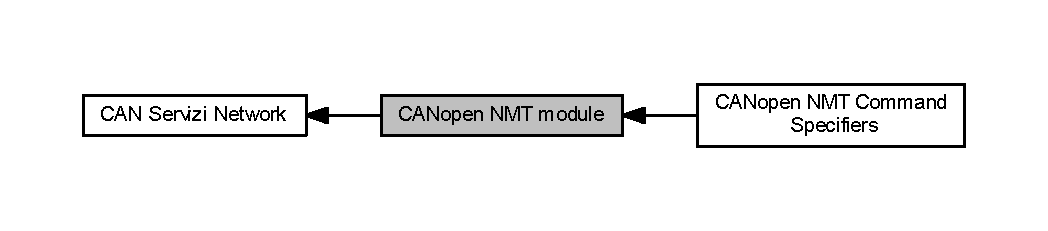
\includegraphics[width=350pt]{group___c_a_nopen___n_m_t__group}
\end{center}
\end{figure}
\subsection*{Modules}
\begin{DoxyCompactItemize}
\item 
\mbox{\hyperlink{group___c_a_nopen___n_m_t__speficications}{C\+A\+Nopen N\+M\+T Command Specifiers}}
\end{DoxyCompactItemize}
\subsection*{Functions}
\begin{DoxyCompactItemize}
\item 
void \mbox{\hyperlink{group___c_a_nopen___n_m_t__group_ga4f3ea874d17be7eefe09f3d8fcd9fc76}{proceed\+N\+M\+Tstate\+Change}} (\mbox{\hyperlink{struct_message}{Message}} $\ast$m)
\begin{DoxyCompactList}\small\item\em According to \mbox{\hyperlink{group___c_a_nopen___n_m_t__speficications}{C\+A\+Nopen N\+MT Command Specifiers}}, upon N\+MT reception from V\+CU master node, S\+CU change current state. \end{DoxyCompactList}\item 
void \mbox{\hyperlink{group___c_a_nopen___n_m_t__group_ga26588b389853484f581977032c0e1021}{slave\+Send\+Boot\+Up}} ()
\begin{DoxyCompactList}\small\item\em This function sends a slave boot-\/up message over C\+AN servizi network. \end{DoxyCompactList}\end{DoxyCompactItemize}


\subsection{Detailed Description}


\subsection{Function Documentation}
\mbox{\Hypertarget{group___c_a_nopen___n_m_t__group_ga4f3ea874d17be7eefe09f3d8fcd9fc76}\label{group___c_a_nopen___n_m_t__group_ga4f3ea874d17be7eefe09f3d8fcd9fc76}} 
\index{C\+A\+Nopen N\+M\+T module@{C\+A\+Nopen N\+M\+T module}!proceed\+N\+M\+Tstate\+Change@{proceed\+N\+M\+Tstate\+Change}}
\index{proceed\+N\+M\+Tstate\+Change@{proceed\+N\+M\+Tstate\+Change}!C\+A\+Nopen N\+M\+T module@{C\+A\+Nopen N\+M\+T module}}
\subsubsection{\texorpdfstring{proceed\+N\+M\+Tstate\+Change()}{proceedNMTstateChange()}}
{\footnotesize\ttfamily void proceed\+N\+M\+Tstate\+Change (\begin{DoxyParamCaption}\item[{\mbox{\hyperlink{struct_message}{Message}} $\ast$}]{m }\end{DoxyParamCaption})}



According to \mbox{\hyperlink{group___c_a_nopen___n_m_t__speficications}{C\+A\+Nopen N\+MT Command Specifiers}}, upon N\+MT reception from V\+CU master node, S\+CU change current state. 

This function manages an N\+MT request from master node on C\+AN servizi network.

\begin{DoxyAuthor}{Author}
Arella Matteo ~\newline
 (mail\+: \href{mailto:arella.1646983@studenti.uniroma1.it}{\tt arella.\+1646983@studenti.\+uniroma1.\+it})
\end{DoxyAuthor}

\begin{DoxyParams}[1]{Parameters}
\mbox{\tt in}  & {\em m} & Received N\+MT message \\
\hline
\end{DoxyParams}


Definition at line 26 of file nmt.\+cpp.

\mbox{\Hypertarget{group___c_a_nopen___n_m_t__group_ga26588b389853484f581977032c0e1021}\label{group___c_a_nopen___n_m_t__group_ga26588b389853484f581977032c0e1021}} 
\index{C\+A\+Nopen N\+M\+T module@{C\+A\+Nopen N\+M\+T module}!slave\+Send\+Boot\+Up@{slave\+Send\+Boot\+Up}}
\index{slave\+Send\+Boot\+Up@{slave\+Send\+Boot\+Up}!C\+A\+Nopen N\+M\+T module@{C\+A\+Nopen N\+M\+T module}}
\subsubsection{\texorpdfstring{slave\+Send\+Boot\+Up()}{slaveSendBootUp()}}
{\footnotesize\ttfamily void slave\+Send\+Boot\+Up (\begin{DoxyParamCaption}{ }\end{DoxyParamCaption})}



This function sends a slave boot-\/up message over C\+AN servizi network. 

\begin{DoxyAuthor}{Author}
Arella Matteo ~\newline
 (mail\+: \href{mailto:arella.1646983@studenti.uniroma1.it}{\tt arella.\+1646983@studenti.\+uniroma1.\+it}) 
\end{DoxyAuthor}


Definition at line 59 of file nmt.\+cpp.


\hypertarget{group___c_a_nopen___p_d_o__module}{}\section{C\+A\+Nopen P\+DO module}
\label{group___c_a_nopen___p_d_o__module}\index{C\+A\+Nopen P\+D\+O module@{C\+A\+Nopen P\+D\+O module}}
Collaboration diagram for C\+A\+Nopen P\+DO module\+:\nopagebreak
\begin{figure}[H]
\begin{center}
\leavevmode
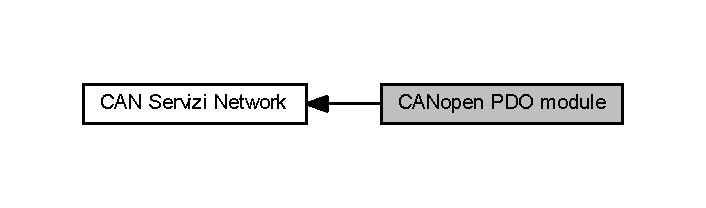
\includegraphics[width=339pt]{group___c_a_nopen___p_d_o__module}
\end{center}
\end{figure}
\subsection*{Functions}
\begin{DoxyCompactItemize}
\item 
void \mbox{\hyperlink{group___c_a_nopen___p_d_o__module_gac0ec660dbbba1d5ab27615147f369caf}{build\+P\+DO}} (uint8\+\_\+t P\+D\+Otype, \mbox{\hyperlink{struct_message}{Message}} $\ast$pdo)
\begin{DoxyCompactList}\small\item\em This function serializes data to send into P\+DO message. \end{DoxyCompactList}\item 
void \mbox{\hyperlink{group___c_a_nopen___p_d_o__module_ga91f92516824d9dc33dc8cf83b34726e1}{proceed\+P\+DO}} (\mbox{\hyperlink{struct_message}{Message}} $\ast$pdo)
\begin{DoxyCompactList}\small\item\em This function manages P\+DO message receive, deserializing data. \end{DoxyCompactList}\end{DoxyCompactItemize}


\subsection{Detailed Description}
Data into P\+D\+Os are configured according \mbox{\hyperlink{_c_a_n_network_page_TPDO_configuration}{T\+P\+D\+O\+\_\+configuration}}. 

\subsection{Function Documentation}
\mbox{\Hypertarget{group___c_a_nopen___p_d_o__module_gac0ec660dbbba1d5ab27615147f369caf}\label{group___c_a_nopen___p_d_o__module_gac0ec660dbbba1d5ab27615147f369caf}} 
\index{C\+A\+Nopen P\+D\+O module@{C\+A\+Nopen P\+D\+O module}!build\+P\+DO@{build\+P\+DO}}
\index{build\+P\+DO@{build\+P\+DO}!C\+A\+Nopen P\+D\+O module@{C\+A\+Nopen P\+D\+O module}}
\subsubsection{\texorpdfstring{build\+P\+D\+O()}{buildPDO()}}
{\footnotesize\ttfamily void build\+P\+DO (\begin{DoxyParamCaption}\item[{uint8\+\_\+t}]{P\+D\+Otype,  }\item[{\mbox{\hyperlink{struct_message}{Message}} $\ast$}]{pdo }\end{DoxyParamCaption})}



This function serializes data to send into P\+DO message. 

\begin{DoxyAuthor}{Author}
Arella Matteo ~\newline
 (mail\+: \href{mailto:arella.1646983@studenti.uniroma1.it}{\tt arella.\+1646983@studenti.\+uniroma1.\+it})
\end{DoxyAuthor}

\begin{DoxyParams}[1]{Parameters}
\mbox{\tt in}  & {\em P\+D\+Otype} & P\+DO type according to \mbox{\hyperlink{group___c_a_nopen___func___codes}{C\+A\+Nopen Function Codes}}. \\
\hline
\mbox{\tt in}  & {\em pdo} & C\+A\+Nopen message to build \\
\hline
\end{DoxyParams}


Definition at line 19 of file pdo.\+cpp.

\mbox{\Hypertarget{group___c_a_nopen___p_d_o__module_ga91f92516824d9dc33dc8cf83b34726e1}\label{group___c_a_nopen___p_d_o__module_ga91f92516824d9dc33dc8cf83b34726e1}} 
\index{C\+A\+Nopen P\+D\+O module@{C\+A\+Nopen P\+D\+O module}!proceed\+P\+DO@{proceed\+P\+DO}}
\index{proceed\+P\+DO@{proceed\+P\+DO}!C\+A\+Nopen P\+D\+O module@{C\+A\+Nopen P\+D\+O module}}
\subsubsection{\texorpdfstring{proceed\+P\+D\+O()}{proceedPDO()}}
{\footnotesize\ttfamily void proceed\+P\+DO (\begin{DoxyParamCaption}\item[{\mbox{\hyperlink{struct_message}{Message}} $\ast$}]{pdo }\end{DoxyParamCaption})}



This function manages P\+DO message receive, deserializing data. 

\begin{DoxyAuthor}{Author}
Arella Matteo ~\newline
 (mail\+: \href{mailto:arella.1646983@studenti.uniroma1.it}{\tt arella.\+1646983@studenti.\+uniroma1.\+it})
\end{DoxyAuthor}

\begin{DoxyParams}[1]{Parameters}
\mbox{\tt in}  & {\em pdo} & C\+A\+Nopen message to manage \\
\hline
\end{DoxyParams}


Definition at line 56 of file pdo.\+cpp.


\hypertarget{group___radio__module}{}\section{Radio module}
\label{group___radio__module}\index{Radio module@{Radio module}}
\subsection*{Macros}
\begin{DoxyCompactItemize}
\item 
\mbox{\Hypertarget{group___radio__module_gaa445a79fc0f7373036c72d198e51f19a}\label{group___radio__module_gaa445a79fc0f7373036c72d198e51f19a}} 
\#define \mbox{\hyperlink{group___radio__module_gaa445a79fc0f7373036c72d198e51f19a}{C\+TR}}~1
\begin{DoxyCompactList}\small\item\em Enable/\+Disable aes C\+TR mode. \end{DoxyCompactList}\item 
\mbox{\Hypertarget{group___radio__module_gaf0e9fea2a1fefbbf655ad908e653fa37}\label{group___radio__module_gaf0e9fea2a1fefbbf655ad908e653fa37}} 
\#define \mbox{\hyperlink{group___radio__module_gaf0e9fea2a1fefbbf655ad908e653fa37}{R\+A\+D\+I\+O\+\_\+\+K\+E\+Y\+\_\+\+B\+I\+TS}}~192
\begin{DoxyCompactList}\small\item\em Aes key length \mbox{[} $bits$\mbox{]}. \end{DoxyCompactList}\item 
\#define \mbox{\hyperlink{group___radio__module_ga2e4ba70a12e464d5b5278c18d28355f8}{J\+S\+O\+N\+\_\+\+B\+U\+F\+F\+E\+R\+\_\+\+S\+I\+ZE}}~J\+S\+O\+N\+\_\+\+O\+B\+J\+E\+C\+T\+\_\+\+S\+I\+ZE(2) + 3 $\ast$ J\+S\+O\+N\+\_\+\+O\+B\+J\+E\+C\+T\+\_\+\+S\+I\+ZE(4) + J\+S\+O\+N\+\_\+\+O\+B\+J\+E\+C\+T\+\_\+\+S\+I\+ZE(5) + 219
\begin{DoxyCompactList}\small\item\em Size of static buffer for J\+S\+ON serialization, generated by \href{https://arduinojson.org/assistant/}{\tt https\+://arduinojson.\+org/assistant/}. Model serialization format\+: \end{DoxyCompactList}\item 
\#define \mbox{\hyperlink{group___radio__module_gae634b89476ef10a9d21eacb0da28cd7b}{C\+I\+P\+H\+E\+R\+\_\+\+M\+A\+X\+\_\+\+L\+E\+N\+G\+TH}}~1024
\begin{DoxyCompactList}\small\item\em Cipher buffer max length (according to \href{https://arduinojson.org/assistant/}{\tt https\+://arduinojson.\+org/assistant/}). \end{DoxyCompactList}\item 
\mbox{\Hypertarget{group___radio__module_ga35dc4d7d23c1b86227ceb68e6ebc4fc2}\label{group___radio__module_ga35dc4d7d23c1b86227ceb68e6ebc4fc2}} 
\#define \mbox{\hyperlink{group___radio__module_ga35dc4d7d23c1b86227ceb68e6ebc4fc2}{I\+V\+\_\+\+L\+EN}}~A\+E\+S\+\_\+\+K\+E\+Y\+L\+EN
\begin{DoxyCompactList}\small\item\em Initialization Vector length. \end{DoxyCompactList}\end{DoxyCompactItemize}
\subsection*{Functions}
\begin{DoxyCompactItemize}
\item 
\mbox{\Hypertarget{group___radio__module_gab473f61dd66af21e8f24b4b95dca0222}\label{group___radio__module_gab473f61dd66af21e8f24b4b95dca0222}} 
R\+F24 \mbox{\hyperlink{group___radio__module_gab473f61dd66af21e8f24b4b95dca0222}{radio}} (R\+A\+D\+I\+O\+\_\+\+C\+E\+\_\+\+P\+IN, R\+A\+D\+I\+O\+\_\+\+C\+S\+N\+\_\+\+P\+IN)
\begin{DoxyCompactList}\small\item\em Radio. \end{DoxyCompactList}\item 
void \mbox{\hyperlink{group___radio__module_ga42ee2daa57d1e88e4ca6c712dba5039a}{encrypt\+\_\+model}} (char $\ast$buffer, char $\ast$\mbox{\hyperlink{group___radio__module_ga352378cd7d5875f33dece696475cb8d4}{iv}}, uint16\+\_\+t plain\+\_\+len, uint16\+\_\+t buffer\+\_\+len)
\begin{DoxyCompactList}\small\item\em Encrypt model for transmit over radio. \end{DoxyCompactList}\item 
volatile char \mbox{\hyperlink{group___radio__module_ga7eb1db79bc6e9408f447ffdc65c09aaa}{generate\+\_\+random\+\_\+char}} ()
\begin{DoxyCompactList}\small\item\em Generate a Cryptgraphically secure pseudorandom number from T\+R\+NG hardware peripheral. \end{DoxyCompactList}\item 
void \mbox{\hyperlink{group___radio__module_ga8d208a46c01313ddc1320256e3ce607d}{generate\+\_\+iv}} (char $\ast$buffer, uint16\+\_\+t len)
\begin{DoxyCompactList}\small\item\em Generate a randomized initialization vector. \end{DoxyCompactList}\item 
void \mbox{\hyperlink{group___radio__module_gad2c532e768a8351b48ffcc95dc56e912}{pkcs7\+\_\+padding}} (char $\ast$buffer, uint16\+\_\+t plain\+\_\+len, uint16\+\_\+t buffer\+\_\+len)
\begin{DoxyCompactList}\small\item\em Perform P\+K\+C\+S7 padding described in R\+FC 5652. \end{DoxyCompactList}\item 
void \mbox{\hyperlink{group___radio__module_ga2cca2e5e5a5f34888f1801e752c29eb3}{byte\+\_\+padding}} (char $\ast$buffer, uint16\+\_\+t plain\+\_\+len, uint16\+\_\+t buffer\+\_\+len)
\begin{DoxyCompactList}\small\item\em Perform I\+S\+O/\+I\+EC 7816-\/4 byte padding. \end{DoxyCompactList}\item 
void \mbox{\hyperlink{group___radio__module_gaaf9aff6a522103cc312457043baf7eca}{radio\+\_\+init}} ()
\begin{DoxyCompactList}\small\item\em Initialize T\+R\+NG (True Random Number Generator) hardware peripheral as a C\+S\+P\+R\+NG (Cryptographically Secure Pseudo-\/\+Random Number Generator) for generate randomized IV. \end{DoxyCompactList}\item 
void \mbox{\hyperlink{group___radio__module_ga5250a82de95a2d4e497dd1c580a92362}{radio\+\_\+send\+\_\+model}} ()
\begin{DoxyCompactList}\small\item\em Actions performed involve\+: \end{DoxyCompactList}\end{DoxyCompactItemize}
\subsection*{Variables}
\begin{DoxyCompactItemize}
\item 
\mbox{\Hypertarget{group___radio__module_gaaebbe13533cac0f28446c13ae32b1cb2}\label{group___radio__module_gaaebbe13533cac0f28446c13ae32b1cb2}} 
volatile bool \mbox{\hyperlink{group___radio__module_gaaebbe13533cac0f28446c13ae32b1cb2}{radio\+\_\+transmit}} = false
\begin{DoxyCompactList}\small\item\em Radio transmit enable flag. \end{DoxyCompactList}\item 
\mbox{\Hypertarget{group___radio__module_gae0c804caa6b80b155884dc4f7a2d9da3}\label{group___radio__module_gae0c804caa6b80b155884dc4f7a2d9da3}} 
char \mbox{\hyperlink{group___radio__module_gae0c804caa6b80b155884dc4f7a2d9da3}{key}} \mbox{[}A\+E\+S\+\_\+\+K\+E\+Y\+L\+EN\mbox{]}
\begin{DoxyCompactList}\small\item\em A\+ES encryption K\+EY. \end{DoxyCompactList}\item 
char \mbox{\hyperlink{group___radio__module_ga352378cd7d5875f33dece696475cb8d4}{iv}} \mbox{[}\mbox{\hyperlink{group___radio__module_ga35dc4d7d23c1b86227ceb68e6ebc4fc2}{I\+V\+\_\+\+L\+EN}}+1\mbox{]}
\begin{DoxyCompactList}\small\item\em A\+ES encryption Initialization Vector. \end{DoxyCompactList}\item 
\mbox{\Hypertarget{group___radio__module_ga4372a894c9299a437425452130748eb8}\label{group___radio__module_ga4372a894c9299a437425452130748eb8}} 
char \mbox{\hyperlink{group___radio__module_ga4372a894c9299a437425452130748eb8}{cipher}} \mbox{[}\mbox{\hyperlink{group___radio__module_gae634b89476ef10a9d21eacb0da28cd7b}{C\+I\+P\+H\+E\+R\+\_\+\+M\+A\+X\+\_\+\+L\+E\+N\+G\+TH}}+1\mbox{]} = \{0\}
\begin{DoxyCompactList}\small\item\em Encrypted model buffer. \end{DoxyCompactList}\item 
\mbox{\Hypertarget{group___radio__module_gafe30685f23b8cbf122ddec37280ba8e4}\label{group___radio__module_gafe30685f23b8cbf122ddec37280ba8e4}} 
const uint64\+\_\+t \mbox{\hyperlink{group___radio__module_gafe30685f23b8cbf122ddec37280ba8e4}{pipe}} = 0x\+E8\+E8\+F0\+F0\+E1\+LL
\begin{DoxyCompactList}\small\item\em Radio writing pipe. \end{DoxyCompactList}\item 
\mbox{\Hypertarget{group___radio__module_gaaebbe13533cac0f28446c13ae32b1cb2}\label{group___radio__module_gaaebbe13533cac0f28446c13ae32b1cb2}} 
volatile bool \mbox{\hyperlink{group___radio__module_gaaebbe13533cac0f28446c13ae32b1cb2}{radio\+\_\+transmit}}
\begin{DoxyCompactList}\small\item\em Radio transmit enable flag. \end{DoxyCompactList}\end{DoxyCompactItemize}


\subsection{Detailed Description}


\subsection{Macro Definition Documentation}
\mbox{\Hypertarget{group___radio__module_gae634b89476ef10a9d21eacb0da28cd7b}\label{group___radio__module_gae634b89476ef10a9d21eacb0da28cd7b}} 
\index{Radio module@{Radio module}!C\+I\+P\+H\+E\+R\+\_\+\+M\+A\+X\+\_\+\+L\+E\+N\+G\+TH@{C\+I\+P\+H\+E\+R\+\_\+\+M\+A\+X\+\_\+\+L\+E\+N\+G\+TH}}
\index{C\+I\+P\+H\+E\+R\+\_\+\+M\+A\+X\+\_\+\+L\+E\+N\+G\+TH@{C\+I\+P\+H\+E\+R\+\_\+\+M\+A\+X\+\_\+\+L\+E\+N\+G\+TH}!Radio module@{Radio module}}
\subsubsection{\texorpdfstring{C\+I\+P\+H\+E\+R\+\_\+\+M\+A\+X\+\_\+\+L\+E\+N\+G\+TH}{CIPHER\_MAX\_LENGTH}}
{\footnotesize\ttfamily \#define C\+I\+P\+H\+E\+R\+\_\+\+M\+A\+X\+\_\+\+L\+E\+N\+G\+TH~1024}



Cipher buffer max length (according to \href{https://arduinojson.org/assistant/}{\tt https\+://arduinojson.\+org/assistant/}). 

\begin{DoxyWarning}{Warning}
Must be a multiple of 16. 
\end{DoxyWarning}


Definition at line 64 of file radio.\+cpp.

\mbox{\Hypertarget{group___radio__module_ga2e4ba70a12e464d5b5278c18d28355f8}\label{group___radio__module_ga2e4ba70a12e464d5b5278c18d28355f8}} 
\index{Radio module@{Radio module}!J\+S\+O\+N\+\_\+\+B\+U\+F\+F\+E\+R\+\_\+\+S\+I\+ZE@{J\+S\+O\+N\+\_\+\+B\+U\+F\+F\+E\+R\+\_\+\+S\+I\+ZE}}
\index{J\+S\+O\+N\+\_\+\+B\+U\+F\+F\+E\+R\+\_\+\+S\+I\+ZE@{J\+S\+O\+N\+\_\+\+B\+U\+F\+F\+E\+R\+\_\+\+S\+I\+ZE}!Radio module@{Radio module}}
\subsubsection{\texorpdfstring{J\+S\+O\+N\+\_\+\+B\+U\+F\+F\+E\+R\+\_\+\+S\+I\+ZE}{JSON\_BUFFER\_SIZE}}
{\footnotesize\ttfamily \#define J\+S\+O\+N\+\_\+\+B\+U\+F\+F\+E\+R\+\_\+\+S\+I\+ZE~J\+S\+O\+N\+\_\+\+O\+B\+J\+E\+C\+T\+\_\+\+S\+I\+ZE(2) + 3 $\ast$ J\+S\+O\+N\+\_\+\+O\+B\+J\+E\+C\+T\+\_\+\+S\+I\+ZE(4) + J\+S\+O\+N\+\_\+\+O\+B\+J\+E\+C\+T\+\_\+\+S\+I\+ZE(5) + 219}



Size of static buffer for J\+S\+ON serialization, generated by \href{https://arduinojson.org/assistant/}{\tt https\+://arduinojson.\+org/assistant/}. Model serialization format\+: 


\begin{DoxyCode}
\{\textcolor{stringliteral}{"pedals"}:\{\textcolor{stringliteral}{"tps1"}:XX,\textcolor{stringliteral}{"tps2"}:XX,\textcolor{stringliteral}{"brake"}:XX,\textcolor{stringliteral}{"apps\_plaus"}:\textcolor{keyword}{true},\textcolor{stringliteral}{"brake\_plaus"}:\textcolor{keyword}{true}\},
 \textcolor{stringliteral}{"suspensions"}:\{\textcolor{stringliteral}{"front\_sx"}:XX,\textcolor{stringliteral}{"front\_dx"}:XX,\textcolor{stringliteral}{"retro\_sx"}:XX,\textcolor{stringliteral}{"retro\_dx"}:XX\},
 \textcolor{stringliteral}{"wheels"}:\{\textcolor{stringliteral}{"front\_sx"}:XXXX,\textcolor{stringliteral}{"front\_dx"}:XXXX,\textcolor{stringliteral}{"retro\_sx"}:XXXX,\textcolor{stringliteral}{"retro\_dx"}:XXXX\},
 \textcolor{stringliteral}{"accelerometers"}:\{\textcolor{stringliteral}{"acc\_x"}:X,\textcolor{stringliteral}{"acc\_z"}:X\}\}
\end{DoxyCode}
 

Definition at line 57 of file radio.\+cpp.



\subsection{Function Documentation}
\mbox{\Hypertarget{group___radio__module_ga2cca2e5e5a5f34888f1801e752c29eb3}\label{group___radio__module_ga2cca2e5e5a5f34888f1801e752c29eb3}} 
\index{Radio module@{Radio module}!byte\+\_\+padding@{byte\+\_\+padding}}
\index{byte\+\_\+padding@{byte\+\_\+padding}!Radio module@{Radio module}}
\subsubsection{\texorpdfstring{byte\+\_\+padding()}{byte\_padding()}}
{\footnotesize\ttfamily void byte\+\_\+padding (\begin{DoxyParamCaption}\item[{char $\ast$}]{buffer,  }\item[{uint16\+\_\+t}]{plain\+\_\+len,  }\item[{uint16\+\_\+t}]{buffer\+\_\+len }\end{DoxyParamCaption})}



Perform I\+S\+O/\+I\+EC 7816-\/4 byte padding. 

\begin{DoxyAuthor}{Author}
Arella Matteo ~\newline
 (mail\+: \href{mailto:arella.1646983@studenti.uniroma1.it}{\tt arella.\+1646983@studenti.\+uniroma1.\+it})
\end{DoxyAuthor}

\begin{DoxyParams}[1]{Parameters}
\mbox{\tt out}  & {\em buffer} & -\/ Buffer \\
\hline
\mbox{\tt in}  & {\em plain\+\_\+len} & -\/ Plain model\textquotesingle{}s length \\
\hline
\mbox{\tt in}  & {\em buffer\+\_\+len} & -\/ Buffer length \\
\hline
\end{DoxyParams}


Definition at line 185 of file radio.\+cpp.

\mbox{\Hypertarget{group___radio__module_ga42ee2daa57d1e88e4ca6c712dba5039a}\label{group___radio__module_ga42ee2daa57d1e88e4ca6c712dba5039a}} 
\index{Radio module@{Radio module}!encrypt\+\_\+model@{encrypt\+\_\+model}}
\index{encrypt\+\_\+model@{encrypt\+\_\+model}!Radio module@{Radio module}}
\subsubsection{\texorpdfstring{encrypt\+\_\+model()}{encrypt\_model()}}
{\footnotesize\ttfamily void encrypt\+\_\+model (\begin{DoxyParamCaption}\item[{char $\ast$}]{buffer,  }\item[{char $\ast$}]{iv,  }\item[{uint16\+\_\+t}]{plain\+\_\+len,  }\item[{uint16\+\_\+t}]{buffer\+\_\+len }\end{DoxyParamCaption})}



Encrypt model for transmit over radio. 

\begin{DoxyAuthor}{Author}
Arella Matteo ~\newline
 (mail\+: \href{mailto:arella.1646983@studenti.uniroma1.it}{\tt arella.\+1646983@studenti.\+uniroma1.\+it})
\end{DoxyAuthor}

\begin{DoxyParams}[1]{Parameters}
\mbox{\tt in,out}  & {\em buffer} & -\/ Buffer to be encrypted \\
\hline
\mbox{\tt in}  & {\em iv} & -\/ Initialisation vector for A\+ES encryption \\
\hline
\mbox{\tt in}  & {\em plain\+\_\+len} & -\/ Plain model\textquotesingle{}s length \\
\hline
\mbox{\tt in}  & {\em buffer\+\_\+len} & -\/ Buffer length \\
\hline
\end{DoxyParams}


Definition at line 193 of file radio.\+cpp.

\mbox{\Hypertarget{group___radio__module_ga8d208a46c01313ddc1320256e3ce607d}\label{group___radio__module_ga8d208a46c01313ddc1320256e3ce607d}} 
\index{Radio module@{Radio module}!generate\+\_\+iv@{generate\+\_\+iv}}
\index{generate\+\_\+iv@{generate\+\_\+iv}!Radio module@{Radio module}}
\subsubsection{\texorpdfstring{generate\+\_\+iv()}{generate\_iv()}}
{\footnotesize\ttfamily void generate\+\_\+iv (\begin{DoxyParamCaption}\item[{char $\ast$}]{buffer,  }\item[{uint16\+\_\+t}]{len }\end{DoxyParamCaption})}



Generate a randomized initialization vector. 

\begin{DoxyAuthor}{Author}
Arella Matteo ~\newline
 (mail\+: \href{mailto:arella.1646983@studenti.uniroma1.it}{\tt arella.\+1646983@studenti.\+uniroma1.\+it})
\end{DoxyAuthor}

\begin{DoxyParams}[1]{Parameters}
\mbox{\tt out}  & {\em buffer} & -\/ Initialisation Vector \\
\hline
\mbox{\tt in}  & {\em len} & -\/ Buffer length \\
\hline
\end{DoxyParams}


Definition at line 152 of file radio.\+cpp.

\mbox{\Hypertarget{group___radio__module_ga7eb1db79bc6e9408f447ffdc65c09aaa}\label{group___radio__module_ga7eb1db79bc6e9408f447ffdc65c09aaa}} 
\index{Radio module@{Radio module}!generate\+\_\+random\+\_\+char@{generate\+\_\+random\+\_\+char}}
\index{generate\+\_\+random\+\_\+char@{generate\+\_\+random\+\_\+char}!Radio module@{Radio module}}
\subsubsection{\texorpdfstring{generate\+\_\+random\+\_\+char()}{generate\_random\_char()}}
{\footnotesize\ttfamily volatile char generate\+\_\+random\+\_\+char (\begin{DoxyParamCaption}{ }\end{DoxyParamCaption})}



Generate a Cryptgraphically secure pseudorandom number from T\+R\+NG hardware peripheral. 

\begin{DoxyAuthor}{Author}
Arella Matteo ~\newline
 (mail\+: \href{mailto:arella.1646983@studenti.uniroma1.it}{\tt arella.\+1646983@studenti.\+uniroma1.\+it})
\end{DoxyAuthor}
\begin{DoxyReturn}{Returns}
Cryptgraphically secure pseudorandom number. 
\end{DoxyReturn}


Definition at line 138 of file radio.\+cpp.

\mbox{\Hypertarget{group___radio__module_gad2c532e768a8351b48ffcc95dc56e912}\label{group___radio__module_gad2c532e768a8351b48ffcc95dc56e912}} 
\index{Radio module@{Radio module}!pkcs7\+\_\+padding@{pkcs7\+\_\+padding}}
\index{pkcs7\+\_\+padding@{pkcs7\+\_\+padding}!Radio module@{Radio module}}
\subsubsection{\texorpdfstring{pkcs7\+\_\+padding()}{pkcs7\_padding()}}
{\footnotesize\ttfamily void pkcs7\+\_\+padding (\begin{DoxyParamCaption}\item[{char $\ast$}]{buffer,  }\item[{uint16\+\_\+t}]{plain\+\_\+len,  }\item[{uint16\+\_\+t}]{buffer\+\_\+len }\end{DoxyParamCaption})}



Perform P\+K\+C\+S7 padding described in R\+FC 5652. 

\begin{DoxyAuthor}{Author}
Arella Matteo ~\newline
 (mail\+: \href{mailto:arella.1646983@studenti.uniroma1.it}{\tt arella.\+1646983@studenti.\+uniroma1.\+it})
\end{DoxyAuthor}

\begin{DoxyParams}[1]{Parameters}
\mbox{\tt out}  & {\em buffer} & -\/ Buffer \\
\hline
\mbox{\tt in}  & {\em plain\+\_\+len} & -\/ Plain model\textquotesingle{}s length \\
\hline
\mbox{\tt in}  & {\em buffer\+\_\+len} & -\/ Buffer length \\
\hline
\end{DoxyParams}


Definition at line 169 of file radio.\+cpp.

\mbox{\Hypertarget{group___radio__module_gaaf9aff6a522103cc312457043baf7eca}\label{group___radio__module_gaaf9aff6a522103cc312457043baf7eca}} 
\index{Radio module@{Radio module}!radio\+\_\+init@{radio\+\_\+init}}
\index{radio\+\_\+init@{radio\+\_\+init}!Radio module@{Radio module}}
\subsubsection{\texorpdfstring{radio\+\_\+init()}{radio\_init()}}
{\footnotesize\ttfamily void radio\+\_\+init (\begin{DoxyParamCaption}{ }\end{DoxyParamCaption})}



Initialize T\+R\+NG (True Random Number Generator) hardware peripheral as a C\+S\+P\+R\+NG (Cryptographically Secure Pseudo-\/\+Random Number Generator) for generate randomized IV. 

Initialize radio.

\begin{DoxyAuthor}{Author}
Arella Matteo ~\newline
 (mail\+: \href{mailto:arella.1646983@studenti.uniroma1.it}{\tt arella.\+1646983@studenti.\+uniroma1.\+it}) 
\end{DoxyAuthor}


Definition at line 213 of file radio.\+cpp.

\mbox{\Hypertarget{group___radio__module_ga5250a82de95a2d4e497dd1c580a92362}\label{group___radio__module_ga5250a82de95a2d4e497dd1c580a92362}} 
\index{Radio module@{Radio module}!radio\+\_\+send\+\_\+model@{radio\+\_\+send\+\_\+model}}
\index{radio\+\_\+send\+\_\+model@{radio\+\_\+send\+\_\+model}!Radio module@{Radio module}}
\subsubsection{\texorpdfstring{radio\+\_\+send\+\_\+model()}{radio\_send\_model()}}
{\footnotesize\ttfamily void radio\+\_\+send\+\_\+model (\begin{DoxyParamCaption}{ }\end{DoxyParamCaption})}



Actions performed involve\+: 

Send vehicle model over radio.


\begin{DoxyItemize}
\item serialize vehicle data into static J\+S\+ON buffer;
\item generate randomised IV;
\item add padding to buffer;
\item encrypt model with 192-\/bit A\+ES encryption (C\+TR mode);
\item encode buffer with base64 encoding;
\item send buffer over radio.
\end{DoxyItemize}

\begin{DoxyAuthor}{Author}
Arella Matteo ~\newline
 (mail\+: \href{mailto:arella.1646983@studenti.uniroma1.it}{\tt arella.\+1646983@studenti.\+uniroma1.\+it})

Arella Matteo ~\newline
 (mail\+: \href{mailto:arella.1646983@studenti.uniroma1.it}{\tt arella.\+1646983@studenti.\+uniroma1.\+it}) 
\end{DoxyAuthor}


Definition at line 236 of file radio.\+cpp.



\subsection{Variable Documentation}
\mbox{\Hypertarget{group___radio__module_ga352378cd7d5875f33dece696475cb8d4}\label{group___radio__module_ga352378cd7d5875f33dece696475cb8d4}} 
\index{Radio module@{Radio module}!iv@{iv}}
\index{iv@{iv}!Radio module@{Radio module}}
\subsubsection{\texorpdfstring{iv}{iv}}
{\footnotesize\ttfamily char iv\mbox{[}\mbox{\hyperlink{group___radio__module_ga35dc4d7d23c1b86227ceb68e6ebc4fc2}{I\+V\+\_\+\+L\+EN}}+1\mbox{]}}



A\+ES encryption Initialization Vector. 

\begin{DoxyWarning}{Warning}
IV must never be reused with the same key 
\end{DoxyWarning}


Definition at line 95 of file radio.\+cpp.


\hypertarget{group___main__group__module}{}\section{Main module}
\label{group___main__group__module}\index{Main module@{Main module}}
\subsection*{Functions}
\begin{DoxyCompactItemize}
\item 
void \mbox{\hyperlink{group___main__group__module_ga4fc01d736fe50cf5b977f755b675f11d}{setup}} ()
\begin{DoxyCompactList}\small\item\em This function perform basic board setup. Upon power-\/up S\+CU (C\+A\+Nopen slave node) goes into initialization. It initializes the entire application, C\+A\+N/\+C\+A\+Nopen interfaces and communication. At the end of the initialization the node tries to transmit boot-\/up message. As soon as it is transmitted successfully, the node switches to Pre-\/operational state. \end{DoxyCompactList}\item 
void \mbox{\hyperlink{group___main__group__module_gafe461d27b9c48d5921c00d521181f12f}{loop}} ()
\begin{DoxyCompactList}\small\item\em This function is called into endless while main loop. It takes care of sending data through radio, if enabled. \end{DoxyCompactList}\end{DoxyCompactItemize}


\subsection{Detailed Description}


\subsection{Function Documentation}
\mbox{\Hypertarget{group___main__group__module_gafe461d27b9c48d5921c00d521181f12f}\label{group___main__group__module_gafe461d27b9c48d5921c00d521181f12f}} 
\index{Main module@{Main module}!loop@{loop}}
\index{loop@{loop}!Main module@{Main module}}
\subsubsection{\texorpdfstring{loop()}{loop()}}
{\footnotesize\ttfamily void loop (\begin{DoxyParamCaption}{ }\end{DoxyParamCaption})}



This function is called into endless while main loop. It takes care of sending data through radio, if enabled. 

\begin{DoxyAuthor}{Author}
Arella Matteo ~\newline
 (mail\+: \href{mailto:arella.1646983@studenti.uniroma1.it}{\tt arella.\+1646983@studenti.\+uniroma1.\+it}) 
\end{DoxyAuthor}


Definition at line 79 of file S\+C\+U.\+ino.

\mbox{\Hypertarget{group___main__group__module_ga4fc01d736fe50cf5b977f755b675f11d}\label{group___main__group__module_ga4fc01d736fe50cf5b977f755b675f11d}} 
\index{Main module@{Main module}!setup@{setup}}
\index{setup@{setup}!Main module@{Main module}}
\subsubsection{\texorpdfstring{setup()}{setup()}}
{\footnotesize\ttfamily void setup (\begin{DoxyParamCaption}{ }\end{DoxyParamCaption})}



This function perform basic board setup. Upon power-\/up S\+CU (C\+A\+Nopen slave node) goes into initialization. It initializes the entire application, C\+A\+N/\+C\+A\+Nopen interfaces and communication. At the end of the initialization the node tries to transmit boot-\/up message. As soon as it is transmitted successfully, the node switches to Pre-\/operational state. 

\begin{DoxyAuthor}{Author}
Arella Matteo ~\newline
 (mail\+: \href{mailto:arella.1646983@studenti.uniroma1.it}{\tt arella.\+1646983@studenti.\+uniroma1.\+it}) 
\end{DoxyAuthor}


Definition at line 59 of file S\+C\+U.\+ino.


\hypertarget{group___board__pinout__group}{}\section{Board pinout}
\label{group___board__pinout__group}\index{Board pinout@{Board pinout}}
Collaboration diagram for Board pinout\+:\nopagebreak
\begin{figure}[H]
\begin{center}
\leavevmode
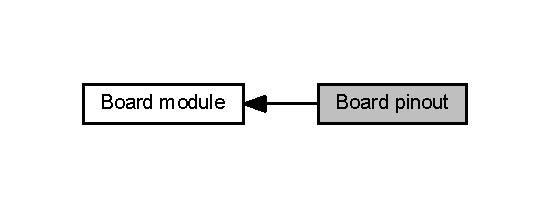
\includegraphics[width=264pt]{group___board__pinout__group}
\end{center}
\end{figure}
\subsection*{Macros}
\begin{DoxyCompactItemize}
\item 
\mbox{\Hypertarget{group___board__pinout__group_gadaeb42d6b221ac2d3e0bd14f05aeefa5}\label{group___board__pinout__group_gadaeb42d6b221ac2d3e0bd14f05aeefa5}} 
\#define \mbox{\hyperlink{group___board__pinout__group_gadaeb42d6b221ac2d3e0bd14f05aeefa5}{C\+A\+N\+\_\+\+P\+O\+RT}}~Can0
\begin{DoxyCompactList}\small\item\em Pin on board dedicated to C\+AN port. \end{DoxyCompactList}\item 
\mbox{\Hypertarget{group___board__pinout__group_gae9aa914854f611488701c96a330b0bd4}\label{group___board__pinout__group_gae9aa914854f611488701c96a330b0bd4}} 
\#define \mbox{\hyperlink{group___board__pinout__group_gae9aa914854f611488701c96a330b0bd4}{T\+P\+S1\+\_\+\+P\+IN}}~A0
\begin{DoxyCompactList}\small\item\em Pin on board dedicated to first A\+P\+PS (tps1) \end{DoxyCompactList}\item 
\mbox{\Hypertarget{group___board__pinout__group_ga99b2a7dadaf495e3c559a46440f9141f}\label{group___board__pinout__group_ga99b2a7dadaf495e3c559a46440f9141f}} 
\#define \mbox{\hyperlink{group___board__pinout__group_ga99b2a7dadaf495e3c559a46440f9141f}{T\+P\+S1\+\_\+\+A\+D\+C\+\_\+\+C\+H\+A\+N\+\_\+\+N\+UM}}~A\+D\+C\+\_\+\+C\+H\+E\+R\+\_\+\+C\+H7
\begin{DoxyCompactList}\small\item\em G\+P\+IO pin on the Atmel S\+A\+M3\+X8E processor corresponding to tps1 signal (A\+D7) \end{DoxyCompactList}\item 
\mbox{\Hypertarget{group___board__pinout__group_gab13a816bae3ca994897fc6f1cb590a67}\label{group___board__pinout__group_gab13a816bae3ca994897fc6f1cb590a67}} 
\#define \mbox{\hyperlink{group___board__pinout__group_gab13a816bae3ca994897fc6f1cb590a67}{T\+P\+S2\+\_\+\+P\+IN}}~A1
\begin{DoxyCompactList}\small\item\em Pin on board dedicated to second A\+P\+PS (tps2) \end{DoxyCompactList}\item 
\mbox{\Hypertarget{group___board__pinout__group_ga4cecb8c10512873904099a1a88d69ed3}\label{group___board__pinout__group_ga4cecb8c10512873904099a1a88d69ed3}} 
\#define \mbox{\hyperlink{group___board__pinout__group_ga4cecb8c10512873904099a1a88d69ed3}{T\+P\+S2\+\_\+\+A\+D\+C\+\_\+\+C\+H\+A\+N\+\_\+\+N\+UM}}~A\+D\+C\+\_\+\+C\+H\+E\+R\+\_\+\+C\+H6
\begin{DoxyCompactList}\small\item\em G\+P\+IO pin on the Atmel S\+A\+M3\+X8E processor corresponding to tps2 signal (A\+D6) \end{DoxyCompactList}\item 
\mbox{\Hypertarget{group___board__pinout__group_gad632b56bf4c6259a390c3db91607078e}\label{group___board__pinout__group_gad632b56bf4c6259a390c3db91607078e}} 
\#define \mbox{\hyperlink{group___board__pinout__group_gad632b56bf4c6259a390c3db91607078e}{B\+R\+A\+K\+E\+\_\+\+P\+IN}}~A2
\begin{DoxyCompactList}\small\item\em Pin on board dedicated to brake pedal position sensor. \end{DoxyCompactList}\item 
\mbox{\Hypertarget{group___board__pinout__group_ga310547321c4a016c4ad19922920fadfd}\label{group___board__pinout__group_ga310547321c4a016c4ad19922920fadfd}} 
\#define \mbox{\hyperlink{group___board__pinout__group_ga310547321c4a016c4ad19922920fadfd}{B\+R\+A\+K\+E\+\_\+\+A\+D\+C\+\_\+\+C\+H\+A\+N\+\_\+\+N\+UM}}~A\+D\+C\+\_\+\+C\+H\+E\+R\+\_\+\+C\+H5
\begin{DoxyCompactList}\small\item\em G\+P\+IO pin on the Atmel S\+A\+M3\+X8E processor corresponding to brake signal (A\+D5) \end{DoxyCompactList}\item 
\mbox{\Hypertarget{group___board__pinout__group_ga26973930bb94d493970560d50ed5388f}\label{group___board__pinout__group_ga26973930bb94d493970560d50ed5388f}} 
\#define \mbox{\hyperlink{group___board__pinout__group_ga26973930bb94d493970560d50ed5388f}{F\+R\+\_\+\+S\+X\+\_\+\+S\+U\+S\+P\+\_\+\+P\+IN}}~A3
\begin{DoxyCompactList}\small\item\em Pin on board dedicated to frontal left suspension sensor. \end{DoxyCompactList}\item 
\mbox{\Hypertarget{group___board__pinout__group_ga3582ac3b04abaa9d74b16da2b18a62f9}\label{group___board__pinout__group_ga3582ac3b04abaa9d74b16da2b18a62f9}} 
\#define \mbox{\hyperlink{group___board__pinout__group_ga3582ac3b04abaa9d74b16da2b18a62f9}{F\+R\+\_\+\+S\+X\+\_\+\+S\+U\+S\+P\+\_\+\+A\+D\+C\+\_\+\+C\+H\+A\+N\+\_\+\+N\+UM}}~A\+D\+C\+\_\+\+C\+H\+E\+R\+\_\+\+C\+H4
\begin{DoxyCompactList}\small\item\em G\+P\+IO pin on the Atmel S\+A\+M3\+X8E processor corresponding to frontal left suspension signal (A\+D4) \end{DoxyCompactList}\item 
\mbox{\Hypertarget{group___board__pinout__group_gac6b52ca09115f1f82aa92ffd31363c05}\label{group___board__pinout__group_gac6b52ca09115f1f82aa92ffd31363c05}} 
\#define \mbox{\hyperlink{group___board__pinout__group_gac6b52ca09115f1f82aa92ffd31363c05}{F\+R\+\_\+\+D\+X\+\_\+\+S\+U\+S\+P\+\_\+\+P\+IN}}~A4
\begin{DoxyCompactList}\small\item\em Pin on board dedicated to frontal right suspension sensor. \end{DoxyCompactList}\item 
\mbox{\Hypertarget{group___board__pinout__group_ga0e9f0303c372af214367d86ad38f660d}\label{group___board__pinout__group_ga0e9f0303c372af214367d86ad38f660d}} 
\#define \mbox{\hyperlink{group___board__pinout__group_ga0e9f0303c372af214367d86ad38f660d}{F\+R\+\_\+\+D\+X\+\_\+\+S\+U\+S\+P\+\_\+\+A\+D\+C\+\_\+\+C\+H\+A\+N\+\_\+\+N\+UM}}~A\+D\+C\+\_\+\+C\+H\+E\+R\+\_\+\+C\+H3
\begin{DoxyCompactList}\small\item\em G\+P\+IO pin on the Atmel S\+A\+M3\+X8E processor corresponding to frontal right suspension signal (A\+D3) \end{DoxyCompactList}\item 
\mbox{\Hypertarget{group___board__pinout__group_ga283872484ffa2d7043a08a80ff7a6cbc}\label{group___board__pinout__group_ga283872484ffa2d7043a08a80ff7a6cbc}} 
\#define \mbox{\hyperlink{group___board__pinout__group_ga283872484ffa2d7043a08a80ff7a6cbc}{F\+R\+\_\+\+S\+X\+\_\+\+P\+W\+\_\+\+P\+IN}}~36
\begin{DoxyCompactList}\small\item\em Pin on board dedicated to frontal left phonic wheel encoder. \end{DoxyCompactList}\item 
\mbox{\Hypertarget{group___board__pinout__group_gad70d75cffb6389aff09c9d9b67a70777}\label{group___board__pinout__group_gad70d75cffb6389aff09c9d9b67a70777}} 
\#define \mbox{\hyperlink{group___board__pinout__group_gad70d75cffb6389aff09c9d9b67a70777}{F\+R\+\_\+\+D\+X\+\_\+\+P\+W\+\_\+\+P\+IN}}~38
\begin{DoxyCompactList}\small\item\em Pin on board dedicated to frontal right phonic wheel encoder. \end{DoxyCompactList}\end{DoxyCompactItemize}


\subsection{Detailed Description}
Board pinout for each sensor, C\+AN port and radio. 
\hypertarget{group___c_a_nopen___f_s_m__module}{}\section{C\+A\+Nopen Finite State Machine module}
\label{group___c_a_nopen___f_s_m__module}\index{C\+A\+Nopen Finite State Machine module@{C\+A\+Nopen Finite State Machine module}}
Collaboration diagram for C\+A\+Nopen Finite State Machine module\+:\nopagebreak
\begin{figure}[H]
\begin{center}
\leavevmode
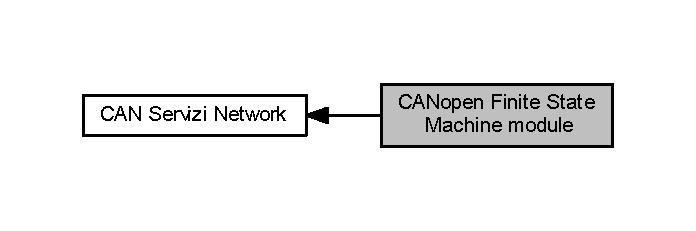
\includegraphics[width=334pt]{group___c_a_nopen___f_s_m__module}
\end{center}
\end{figure}
\subsection*{Typedefs}
\begin{DoxyCompactItemize}
\item 
typedef enum \mbox{\hyperlink{group___c_a_nopen___f_s_m__module_ga3136d2815abe9d284f985e0a7ec68646}{enum\+\_\+node\+State}} \mbox{\hyperlink{group___c_a_nopen___f_s_m__module_ga5891f63a4c9243179838389a93d084e2}{e\+\_\+node\+State}}
\end{DoxyCompactItemize}
\subsection*{Enumerations}
\begin{DoxyCompactItemize}
\item 
enum \mbox{\hyperlink{group___c_a_nopen___f_s_m__module_ga3136d2815abe9d284f985e0a7ec68646}{enum\+\_\+node\+State}} \{ \newline
\mbox{\hyperlink{group___c_a_nopen___f_s_m__module_gga3136d2815abe9d284f985e0a7ec68646aeb3ae26d7a1629aa0fc6c83f46306cf5}{Initialisation}} = 0x00, 
\mbox{\hyperlink{group___c_a_nopen___f_s_m__module_gga3136d2815abe9d284f985e0a7ec68646a84ab0fbbb76a8c897feb1cd806d56443}{Disconnected}} = 0x01, 
\mbox{\hyperlink{group___c_a_nopen___f_s_m__module_gga3136d2815abe9d284f985e0a7ec68646a6ea90df6fe966852496b4846da497fb0}{Connecting}} = 0x02, 
\mbox{\hyperlink{group___c_a_nopen___f_s_m__module_gga3136d2815abe9d284f985e0a7ec68646a95fc3c631fbad8ca3dc8d5b69a3e0d5b}{Preparing}} = 0x02, 
\newline
\mbox{\hyperlink{group___c_a_nopen___f_s_m__module_gga3136d2815abe9d284f985e0a7ec68646a4d049c6d45e08a294523df186ad77a75}{Stopped}} = 0x04, 
\mbox{\hyperlink{group___c_a_nopen___f_s_m__module_gga3136d2815abe9d284f985e0a7ec68646aa80594b1522cb686b981f56bbec45124}{Operational}} = 0x05, 
\mbox{\hyperlink{group___c_a_nopen___f_s_m__module_gga3136d2815abe9d284f985e0a7ec68646ac747c16a9c4d7dec65cdab6e38df99b7}{Pre\+\_\+operational}} = 0x7F, 
\mbox{\hyperlink{group___c_a_nopen___f_s_m__module_gga3136d2815abe9d284f985e0a7ec68646acb4b5cb64be091d76f846380eb0afe59}{Unknown\+\_\+state}} = 0x0F
 \}
\end{DoxyCompactItemize}
\subsection*{Functions}
\begin{DoxyCompactItemize}
\item 
\mbox{\hyperlink{group___c_a_nopen___f_s_m__module_ga5891f63a4c9243179838389a93d084e2}{e\+\_\+node\+State}} \mbox{\hyperlink{group___c_a_nopen___f_s_m__module_ga2802a8c3f0174f4e54dd2381968212a0}{get\+State}} ()
\begin{DoxyCompactList}\small\item\em Return current state on the \mbox{\hyperlink{_f_s_m_page}{Finite State Machine (F\+SM)}}. \end{DoxyCompactList}\item 
void \mbox{\hyperlink{group___c_a_nopen___f_s_m__module_ga47cb7615bbcf2c96cc4a7656f9a76bab}{set\+State}} (\mbox{\hyperlink{group___c_a_nopen___f_s_m__module_ga5891f63a4c9243179838389a93d084e2}{e\+\_\+node\+State}} new\+State)
\begin{DoxyCompactList}\small\item\em Set current state on the \mbox{\hyperlink{_f_s_m_page}{Finite State Machine (F\+SM)}}. \end{DoxyCompactList}\item 
void \mbox{\hyperlink{group___c_a_nopen___f_s_m__module_gabbbb23c086599a8d9432a2121ee82192}{can\+Dispatch}} (\mbox{\hyperlink{struct_message}{Message}} $\ast$m)
\begin{DoxyCompactList}\small\item\em Called by driver when receiving C\+A\+Nopen messages. \end{DoxyCompactList}\item 
void \mbox{\hyperlink{group___c_a_nopen___f_s_m__module_gadfffb3be7aa80aea898ada67e93d2388}{initialisation}} ()
\begin{DoxyCompactList}\small\item\em Initialize \mbox{\hyperlink{group___board__model__group}{Board module}}. If rear S\+CU firmware is selected (according to \mbox{\hyperlink{group___s_c_u__firmware__selection}{S\+CU firmware selection}}) radio is initialized. It initializes the entire application, C\+A\+N/\+C\+A\+Nopen interfaces and communication. \end{DoxyCompactList}\item 
void \mbox{\hyperlink{group___c_a_nopen___f_s_m__module_gaf9e8e3744244bcb2f8b6a8583c0bec0c}{pre\+Operational}} ()
\begin{DoxyCompactList}\small\item\em pre\+Operational state task on the F\+SM. \end{DoxyCompactList}\item 
void \mbox{\hyperlink{group___c_a_nopen___f_s_m__module_ga003b28d176774c489577f471a7b5f946}{operational}} ()
\begin{DoxyCompactList}\small\item\em Start timer for periodic T\+P\+DO transmit according to \mbox{\hyperlink{_c_a_n_network_page}{C\+AN Servizi network}}. \end{DoxyCompactList}\item 
void \mbox{\hyperlink{group___c_a_nopen___f_s_m__module_gad134c6ce7186d3f2e9cb314839fd63ad}{stopped}} ()
\begin{DoxyCompactList}\small\item\em Stop timer for periodic T\+P\+DO transmit according to \mbox{\hyperlink{_c_a_n_network_page}{C\+AN Servizi network}}. \end{DoxyCompactList}\end{DoxyCompactItemize}
\subsection*{Variables}
\begin{DoxyCompactItemize}
\item 
\mbox{\Hypertarget{group___c_a_nopen___f_s_m__module_ga924e56dabe104382db4ee1a3bb507ed9}\label{group___c_a_nopen___f_s_m__module_ga924e56dabe104382db4ee1a3bb507ed9}} 
volatile \mbox{\hyperlink{group___c_a_nopen___f_s_m__module_ga5891f63a4c9243179838389a93d084e2}{e\+\_\+node\+State}} \mbox{\hyperlink{group___c_a_nopen___f_s_m__module_ga924e56dabe104382db4ee1a3bb507ed9}{current\+\_\+state}} = \mbox{\hyperlink{group___c_a_nopen___f_s_m__module_gga3136d2815abe9d284f985e0a7ec68646aeb3ae26d7a1629aa0fc6c83f46306cf5}{Initialisation}}
\begin{DoxyCompactList}\small\item\em Current state of F\+SM. \end{DoxyCompactList}\end{DoxyCompactItemize}


\subsection{Detailed Description}


\subsection{Typedef Documentation}
\mbox{\Hypertarget{group___c_a_nopen___f_s_m__module_ga5891f63a4c9243179838389a93d084e2}\label{group___c_a_nopen___f_s_m__module_ga5891f63a4c9243179838389a93d084e2}} 
\index{C\+A\+Nopen Finite State Machine module@{C\+A\+Nopen Finite State Machine module}!e\+\_\+node\+State@{e\+\_\+node\+State}}
\index{e\+\_\+node\+State@{e\+\_\+node\+State}!C\+A\+Nopen Finite State Machine module@{C\+A\+Nopen Finite State Machine module}}
\subsubsection{\texorpdfstring{e\+\_\+node\+State}{e\_nodeState}}
{\footnotesize\ttfamily typedef enum \mbox{\hyperlink{group___c_a_nopen___f_s_m__module_ga3136d2815abe9d284f985e0a7ec68646}{enum\+\_\+node\+State}} \mbox{\hyperlink{group___c_a_nopen___f_s_m__module_ga5891f63a4c9243179838389a93d084e2}{e\+\_\+node\+State}}}

F\+SM states typedef 

Definition at line 55 of file states.\+h.



\subsection{Enumeration Type Documentation}
\mbox{\Hypertarget{group___c_a_nopen___f_s_m__module_ga3136d2815abe9d284f985e0a7ec68646}\label{group___c_a_nopen___f_s_m__module_ga3136d2815abe9d284f985e0a7ec68646}} 
\index{C\+A\+Nopen Finite State Machine module@{C\+A\+Nopen Finite State Machine module}!enum\+\_\+node\+State@{enum\+\_\+node\+State}}
\index{enum\+\_\+node\+State@{enum\+\_\+node\+State}!C\+A\+Nopen Finite State Machine module@{C\+A\+Nopen Finite State Machine module}}
\subsubsection{\texorpdfstring{enum\+\_\+node\+State}{enum\_nodeState}}
{\footnotesize\ttfamily enum \mbox{\hyperlink{group___c_a_nopen___f_s_m__module_ga3136d2815abe9d284f985e0a7ec68646}{enum\+\_\+node\+State}}}

F\+SM states enum \begin{DoxyEnumFields}{Enumerator}
\raisebox{\heightof{T}}[0pt][0pt]{\index{Initialisation@{Initialisation}!C\+A\+Nopen Finite State Machine module@{C\+A\+Nopen Finite State Machine module}}\index{C\+A\+Nopen Finite State Machine module@{C\+A\+Nopen Finite State Machine module}!Initialisation@{Initialisation}}}\mbox{\Hypertarget{group___c_a_nopen___f_s_m__module_gga3136d2815abe9d284f985e0a7ec68646aeb3ae26d7a1629aa0fc6c83f46306cf5}\label{group___c_a_nopen___f_s_m__module_gga3136d2815abe9d284f985e0a7ec68646aeb3ae26d7a1629aa0fc6c83f46306cf5}} 
Initialisation&Initialisation state \\
\hline

\raisebox{\heightof{T}}[0pt][0pt]{\index{Disconnected@{Disconnected}!C\+A\+Nopen Finite State Machine module@{C\+A\+Nopen Finite State Machine module}}\index{C\+A\+Nopen Finite State Machine module@{C\+A\+Nopen Finite State Machine module}!Disconnected@{Disconnected}}}\mbox{\Hypertarget{group___c_a_nopen___f_s_m__module_gga3136d2815abe9d284f985e0a7ec68646a84ab0fbbb76a8c897feb1cd806d56443}\label{group___c_a_nopen___f_s_m__module_gga3136d2815abe9d284f985e0a7ec68646a84ab0fbbb76a8c897feb1cd806d56443}} 
Disconnected&Disconnected state \\
\hline

\raisebox{\heightof{T}}[0pt][0pt]{\index{Connecting@{Connecting}!C\+A\+Nopen Finite State Machine module@{C\+A\+Nopen Finite State Machine module}}\index{C\+A\+Nopen Finite State Machine module@{C\+A\+Nopen Finite State Machine module}!Connecting@{Connecting}}}\mbox{\Hypertarget{group___c_a_nopen___f_s_m__module_gga3136d2815abe9d284f985e0a7ec68646a6ea90df6fe966852496b4846da497fb0}\label{group___c_a_nopen___f_s_m__module_gga3136d2815abe9d284f985e0a7ec68646a6ea90df6fe966852496b4846da497fb0}} 
Connecting&Connecting state \\
\hline

\raisebox{\heightof{T}}[0pt][0pt]{\index{Preparing@{Preparing}!C\+A\+Nopen Finite State Machine module@{C\+A\+Nopen Finite State Machine module}}\index{C\+A\+Nopen Finite State Machine module@{C\+A\+Nopen Finite State Machine module}!Preparing@{Preparing}}}\mbox{\Hypertarget{group___c_a_nopen___f_s_m__module_gga3136d2815abe9d284f985e0a7ec68646a95fc3c631fbad8ca3dc8d5b69a3e0d5b}\label{group___c_a_nopen___f_s_m__module_gga3136d2815abe9d284f985e0a7ec68646a95fc3c631fbad8ca3dc8d5b69a3e0d5b}} 
Preparing&Preparing state \\
\hline

\raisebox{\heightof{T}}[0pt][0pt]{\index{Stopped@{Stopped}!C\+A\+Nopen Finite State Machine module@{C\+A\+Nopen Finite State Machine module}}\index{C\+A\+Nopen Finite State Machine module@{C\+A\+Nopen Finite State Machine module}!Stopped@{Stopped}}}\mbox{\Hypertarget{group___c_a_nopen___f_s_m__module_gga3136d2815abe9d284f985e0a7ec68646a4d049c6d45e08a294523df186ad77a75}\label{group___c_a_nopen___f_s_m__module_gga3136d2815abe9d284f985e0a7ec68646a4d049c6d45e08a294523df186ad77a75}} 
Stopped&Stopped state \\
\hline

\raisebox{\heightof{T}}[0pt][0pt]{\index{Operational@{Operational}!C\+A\+Nopen Finite State Machine module@{C\+A\+Nopen Finite State Machine module}}\index{C\+A\+Nopen Finite State Machine module@{C\+A\+Nopen Finite State Machine module}!Operational@{Operational}}}\mbox{\Hypertarget{group___c_a_nopen___f_s_m__module_gga3136d2815abe9d284f985e0a7ec68646aa80594b1522cb686b981f56bbec45124}\label{group___c_a_nopen___f_s_m__module_gga3136d2815abe9d284f985e0a7ec68646aa80594b1522cb686b981f56bbec45124}} 
Operational&Operational state \\
\hline

\raisebox{\heightof{T}}[0pt][0pt]{\index{Pre\+\_\+operational@{Pre\+\_\+operational}!C\+A\+Nopen Finite State Machine module@{C\+A\+Nopen Finite State Machine module}}\index{C\+A\+Nopen Finite State Machine module@{C\+A\+Nopen Finite State Machine module}!Pre\+\_\+operational@{Pre\+\_\+operational}}}\mbox{\Hypertarget{group___c_a_nopen___f_s_m__module_gga3136d2815abe9d284f985e0a7ec68646ac747c16a9c4d7dec65cdab6e38df99b7}\label{group___c_a_nopen___f_s_m__module_gga3136d2815abe9d284f985e0a7ec68646ac747c16a9c4d7dec65cdab6e38df99b7}} 
Pre\+\_\+operational&Pre\+Operational state \\
\hline

\raisebox{\heightof{T}}[0pt][0pt]{\index{Unknown\+\_\+state@{Unknown\+\_\+state}!C\+A\+Nopen Finite State Machine module@{C\+A\+Nopen Finite State Machine module}}\index{C\+A\+Nopen Finite State Machine module@{C\+A\+Nopen Finite State Machine module}!Unknown\+\_\+state@{Unknown\+\_\+state}}}\mbox{\Hypertarget{group___c_a_nopen___f_s_m__module_gga3136d2815abe9d284f985e0a7ec68646acb4b5cb64be091d76f846380eb0afe59}\label{group___c_a_nopen___f_s_m__module_gga3136d2815abe9d284f985e0a7ec68646acb4b5cb64be091d76f846380eb0afe59}} 
Unknown\+\_\+state&Unknown state \\
\hline

\end{DoxyEnumFields}


Definition at line 43 of file states.\+h.



\subsection{Function Documentation}
\mbox{\Hypertarget{group___c_a_nopen___f_s_m__module_gabbbb23c086599a8d9432a2121ee82192}\label{group___c_a_nopen___f_s_m__module_gabbbb23c086599a8d9432a2121ee82192}} 
\index{C\+A\+Nopen Finite State Machine module@{C\+A\+Nopen Finite State Machine module}!can\+Dispatch@{can\+Dispatch}}
\index{can\+Dispatch@{can\+Dispatch}!C\+A\+Nopen Finite State Machine module@{C\+A\+Nopen Finite State Machine module}}
\subsubsection{\texorpdfstring{can\+Dispatch()}{canDispatch()}}
{\footnotesize\ttfamily void can\+Dispatch (\begin{DoxyParamCaption}\item[{\mbox{\hyperlink{struct_message}{Message}} $\ast$}]{m }\end{DoxyParamCaption})}



Called by driver when receiving C\+A\+Nopen messages. 

\begin{DoxyAuthor}{Author}
Arella Matteo ~\newline
 (mail\+: \href{mailto:arella.1646983@studenti.uniroma1.it}{\tt arella.\+1646983@studenti.\+uniroma1.\+it})
\end{DoxyAuthor}

\begin{DoxyParams}[1]{Parameters}
\mbox{\tt in}  & {\em m} & Received C\+A\+Nopen message \\
\hline
\end{DoxyParams}


Definition at line 45 of file states.\+cpp.

\mbox{\Hypertarget{group___c_a_nopen___f_s_m__module_ga2802a8c3f0174f4e54dd2381968212a0}\label{group___c_a_nopen___f_s_m__module_ga2802a8c3f0174f4e54dd2381968212a0}} 
\index{C\+A\+Nopen Finite State Machine module@{C\+A\+Nopen Finite State Machine module}!get\+State@{get\+State}}
\index{get\+State@{get\+State}!C\+A\+Nopen Finite State Machine module@{C\+A\+Nopen Finite State Machine module}}
\subsubsection{\texorpdfstring{get\+State()}{getState()}}
{\footnotesize\ttfamily \mbox{\hyperlink{group___c_a_nopen___f_s_m__module_ga5891f63a4c9243179838389a93d084e2}{e\+\_\+node\+State}} get\+State (\begin{DoxyParamCaption}{ }\end{DoxyParamCaption})}



Return current state on the \mbox{\hyperlink{_f_s_m_page}{Finite State Machine (F\+SM)}}. 

\begin{DoxyAuthor}{Author}
Arella Matteo ~\newline
 (mail\+: \href{mailto:arella.1646983@studenti.uniroma1.it}{\tt arella.\+1646983@studenti.\+uniroma1.\+it})
\end{DoxyAuthor}
\begin{DoxyReturn}{Returns}
current state on the F\+SM 
\end{DoxyReturn}


Definition at line 35 of file states.\+cpp.

\mbox{\Hypertarget{group___c_a_nopen___f_s_m__module_gadfffb3be7aa80aea898ada67e93d2388}\label{group___c_a_nopen___f_s_m__module_gadfffb3be7aa80aea898ada67e93d2388}} 
\index{C\+A\+Nopen Finite State Machine module@{C\+A\+Nopen Finite State Machine module}!initialisation@{initialisation}}
\index{initialisation@{initialisation}!C\+A\+Nopen Finite State Machine module@{C\+A\+Nopen Finite State Machine module}}
\subsubsection{\texorpdfstring{initialisation()}{initialisation()}}
{\footnotesize\ttfamily void initialisation (\begin{DoxyParamCaption}{ }\end{DoxyParamCaption})}



Initialize \mbox{\hyperlink{group___board__model__group}{Board module}}. If rear S\+CU firmware is selected (according to \mbox{\hyperlink{group___s_c_u__firmware__selection}{S\+CU firmware selection}}) radio is initialized. It initializes the entire application, C\+A\+N/\+C\+A\+Nopen interfaces and communication. 

Initialisation state task on the F\+SM.

\begin{DoxyAuthor}{Author}
Arella Matteo ~\newline
 (mail\+: \href{mailto:arella.1646983@studenti.uniroma1.it}{\tt arella.\+1646983@studenti.\+uniroma1.\+it}) 
\end{DoxyAuthor}


Definition at line 71 of file states.\+cpp.

\mbox{\Hypertarget{group___c_a_nopen___f_s_m__module_ga003b28d176774c489577f471a7b5f946}\label{group___c_a_nopen___f_s_m__module_ga003b28d176774c489577f471a7b5f946}} 
\index{C\+A\+Nopen Finite State Machine module@{C\+A\+Nopen Finite State Machine module}!operational@{operational}}
\index{operational@{operational}!C\+A\+Nopen Finite State Machine module@{C\+A\+Nopen Finite State Machine module}}
\subsubsection{\texorpdfstring{operational()}{operational()}}
{\footnotesize\ttfamily void operational (\begin{DoxyParamCaption}{ }\end{DoxyParamCaption})}



Start timer for periodic T\+P\+DO transmit according to \mbox{\hyperlink{_c_a_n_network_page}{C\+AN Servizi network}}. 

Operational state task on the F\+SM.

\begin{DoxyAuthor}{Author}
Arella Matteo ~\newline
 (mail\+: \href{mailto:arella.1646983@studenti.uniroma1.it}{\tt arella.\+1646983@studenti.\+uniroma1.\+it}) 
\end{DoxyAuthor}


Definition at line 95 of file states.\+cpp.

\mbox{\Hypertarget{group___c_a_nopen___f_s_m__module_gaf9e8e3744244bcb2f8b6a8583c0bec0c}\label{group___c_a_nopen___f_s_m__module_gaf9e8e3744244bcb2f8b6a8583c0bec0c}} 
\index{C\+A\+Nopen Finite State Machine module@{C\+A\+Nopen Finite State Machine module}!pre\+Operational@{pre\+Operational}}
\index{pre\+Operational@{pre\+Operational}!C\+A\+Nopen Finite State Machine module@{C\+A\+Nopen Finite State Machine module}}
\subsubsection{\texorpdfstring{pre\+Operational()}{preOperational()}}
{\footnotesize\ttfamily void pre\+Operational (\begin{DoxyParamCaption}{ }\end{DoxyParamCaption})}



pre\+Operational state task on the F\+SM. 

\begin{DoxyAuthor}{Author}
Arella Matteo ~\newline
 (mail\+: \href{mailto:arella.1646983@studenti.uniroma1.it}{\tt arella.\+1646983@studenti.\+uniroma1.\+it}) 
\end{DoxyAuthor}


Definition at line 83 of file states.\+cpp.

\mbox{\Hypertarget{group___c_a_nopen___f_s_m__module_ga47cb7615bbcf2c96cc4a7656f9a76bab}\label{group___c_a_nopen___f_s_m__module_ga47cb7615bbcf2c96cc4a7656f9a76bab}} 
\index{C\+A\+Nopen Finite State Machine module@{C\+A\+Nopen Finite State Machine module}!set\+State@{set\+State}}
\index{set\+State@{set\+State}!C\+A\+Nopen Finite State Machine module@{C\+A\+Nopen Finite State Machine module}}
\subsubsection{\texorpdfstring{set\+State()}{setState()}}
{\footnotesize\ttfamily void set\+State (\begin{DoxyParamCaption}\item[{\mbox{\hyperlink{group___c_a_nopen___f_s_m__module_ga5891f63a4c9243179838389a93d084e2}{e\+\_\+node\+State}}}]{new\+State }\end{DoxyParamCaption})}



Set current state on the \mbox{\hyperlink{_f_s_m_page}{Finite State Machine (F\+SM)}}. 

\begin{DoxyAuthor}{Author}
Arella Matteo ~\newline
 (mail\+: \href{mailto:arella.1646983@studenti.uniroma1.it}{\tt arella.\+1646983@studenti.\+uniroma1.\+it})
\end{DoxyAuthor}

\begin{DoxyParams}[1]{Parameters}
\mbox{\tt in}  & {\em new\+State} & New state transition \\
\hline
\end{DoxyParams}


Definition at line 40 of file states.\+cpp.

\mbox{\Hypertarget{group___c_a_nopen___f_s_m__module_gad134c6ce7186d3f2e9cb314839fd63ad}\label{group___c_a_nopen___f_s_m__module_gad134c6ce7186d3f2e9cb314839fd63ad}} 
\index{C\+A\+Nopen Finite State Machine module@{C\+A\+Nopen Finite State Machine module}!stopped@{stopped}}
\index{stopped@{stopped}!C\+A\+Nopen Finite State Machine module@{C\+A\+Nopen Finite State Machine module}}
\subsubsection{\texorpdfstring{stopped()}{stopped()}}
{\footnotesize\ttfamily void stopped (\begin{DoxyParamCaption}{ }\end{DoxyParamCaption})}



Stop timer for periodic T\+P\+DO transmit according to \mbox{\hyperlink{_c_a_n_network_page}{C\+AN Servizi network}}. 

Stopped state task on the F\+SM.

\begin{DoxyAuthor}{Author}
Arella Matteo ~\newline
 (mail\+: \href{mailto:arella.1646983@studenti.uniroma1.it}{\tt arella.\+1646983@studenti.\+uniroma1.\+it}) 
\end{DoxyAuthor}


Definition at line 108 of file states.\+cpp.


\hypertarget{group___c_a_nopen__timer__module}{}\section{C\+A\+Nopen Timer module}
\label{group___c_a_nopen__timer__module}\index{C\+A\+Nopen Timer module@{C\+A\+Nopen Timer module}}
Collaboration diagram for C\+A\+Nopen Timer module\+:\nopagebreak
\begin{figure}[H]
\begin{center}
\leavevmode
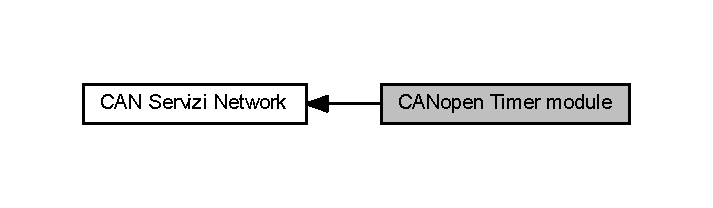
\includegraphics[width=342pt]{group___c_a_nopen__timer__module}
\end{center}
\end{figure}
\subsection*{Macros}
\begin{DoxyCompactItemize}
\item 
\mbox{\Hypertarget{group___c_a_nopen__timer__module_ga5bb58b675652213c5b20458ab611f9fb}\label{group___c_a_nopen__timer__module_ga5bb58b675652213c5b20458ab611f9fb}} 
\#define \mbox{\hyperlink{group___c_a_nopen__timer__module_ga5bb58b675652213c5b20458ab611f9fb}{S\+C\+U\+\_\+\+F\+R\+O\+N\+T\+\_\+\+F\+I\+R\+S\+T\+\_\+\+S\+L\+OT}}~0
\begin{DoxyCompactList}\small\item\em First time slot for $SCU_{Frontal}$. \end{DoxyCompactList}\item 
\mbox{\Hypertarget{group___c_a_nopen__timer__module_gae5482bf356c02f4af400a276980e8bbc}\label{group___c_a_nopen__timer__module_gae5482bf356c02f4af400a276980e8bbc}} 
\#define \mbox{\hyperlink{group___c_a_nopen__timer__module_gae5482bf356c02f4af400a276980e8bbc}{S\+C\+U\+\_\+\+F\+R\+O\+N\+T\+\_\+\+S\+E\+C\+O\+N\+D\+\_\+\+S\+L\+OT}}~1
\begin{DoxyCompactList}\small\item\em Second time slot for $SCU_{Frontal}$. \end{DoxyCompactList}\item 
\mbox{\Hypertarget{group___c_a_nopen__timer__module_gaf913e12f6687d34f5ad716d130416dc8}\label{group___c_a_nopen__timer__module_gaf913e12f6687d34f5ad716d130416dc8}} 
\#define \mbox{\hyperlink{group___c_a_nopen__timer__module_gaf913e12f6687d34f5ad716d130416dc8}{S\+C\+U\+\_\+\+R\+E\+A\+R\+\_\+\+S\+L\+OT}}~2
\begin{DoxyCompactList}\small\item\em Time slot for $SCU_{Rear}$. \end{DoxyCompactList}\item 
\mbox{\Hypertarget{group___c_a_nopen__timer__module_ga266f975ed5b87594263f8a2bf8257cdf}\label{group___c_a_nopen__timer__module_ga266f975ed5b87594263f8a2bf8257cdf}} 
\#define \mbox{\hyperlink{group___c_a_nopen__timer__module_ga266f975ed5b87594263f8a2bf8257cdf}{T\+C\+S\+\_\+\+S\+L\+OT}}~3
\begin{DoxyCompactList}\small\item\em Time slot for $TCU$. \end{DoxyCompactList}\item 
\mbox{\Hypertarget{group___c_a_nopen__timer__module_gaab4fadccdeb20ba1f44ed01296b7e560}\label{group___c_a_nopen__timer__module_gaab4fadccdeb20ba1f44ed01296b7e560}} 
\#define \mbox{\hyperlink{group___c_a_nopen__timer__module_gaab4fadccdeb20ba1f44ed01296b7e560}{T\+I\+M\+E\+\_\+\+S\+L\+O\+T\+\_\+\+M\+A\+SK}}~3
\begin{DoxyCompactList}\small\item\em Time slot mask. \end{DoxyCompactList}\item 
\mbox{\Hypertarget{group___c_a_nopen__timer__module_gaf3ebceeca1e0dded3572b4367c5d6413}\label{group___c_a_nopen__timer__module_gaf3ebceeca1e0dded3572b4367c5d6413}} 
\#define \mbox{\hyperlink{group___c_a_nopen__timer__module_gaf3ebceeca1e0dded3572b4367c5d6413}{R\+A\+D\+I\+O\+\_\+\+S\+L\+O\+T\+\_\+\+M\+A\+SK}}~7
\begin{DoxyCompactList}\small\item\em Radio submit slot mask\+: number of $SCU_{Rear}$ time slots between one submit and successive one (\mbox{\hyperlink{group___common__defines__group_ga09c95853fd002fab968d94c5bc44e823}{T\+I\+M\+E\+\_\+\+S\+L\+O\+T\+\_\+\+P\+E\+R\+I\+OD}} $\ast$ \mbox{\hyperlink{group___c_a_nopen__timer__module_gaf3ebceeca1e0dded3572b4367c5d6413}{R\+A\+D\+I\+O\+\_\+\+S\+L\+O\+T\+\_\+\+M\+A\+SK}} $\ast$ num. time slots between previous and current $SCU_{Rear}$) \end{DoxyCompactList}\end{DoxyCompactItemize}
\subsection*{Functions}
\begin{DoxyCompactItemize}
\item 
void \mbox{\hyperlink{group___c_a_nopen__timer__module_gafa75192a3238525618f8cb83004930cc}{Time\+Dispatch}} ()
\begin{DoxyCompactList}\small\item\em Dispatch time slot for each C\+A\+Nopen node according to \mbox{\hyperlink{_c_a_n_network_page_TPDO_Timer}{T\+P\+D\+O\+\_\+\+Timer}}. \end{DoxyCompactList}\item 
void \mbox{\hyperlink{group___c_a_nopen__timer__module_gaf927959e78504fd1afe1be1e10791ae0}{timer\+Init}} ()
\begin{DoxyCompactList}\small\item\em Initialize timer for periodic submit of T\+P\+D\+Os. \end{DoxyCompactList}\item 
void \mbox{\hyperlink{group___c_a_nopen__timer__module_gaddf92f4b7b741f7b9fbc827d2e4f2a8b}{timer\+Start}} ()
\begin{DoxyCompactList}\small\item\em Start timer for periodic submit of T\+P\+D\+Os. \end{DoxyCompactList}\item 
void \mbox{\hyperlink{group___c_a_nopen__timer__module_gaecc39b6c4a6a4d79a46ac2b6371221c5}{timer\+Stop}} ()
\begin{DoxyCompactList}\small\item\em Stop timer for periodic submit of T\+P\+D\+Os. \end{DoxyCompactList}\end{DoxyCompactItemize}
\subsection*{Variables}
\begin{DoxyCompactItemize}
\item 
\mbox{\Hypertarget{group___c_a_nopen__timer__module_ga38a43dbb3c9d41a62672688eb57fa33f}\label{group___c_a_nopen__timer__module_ga38a43dbb3c9d41a62672688eb57fa33f}} 
volatile uint8\+\_\+t \mbox{\hyperlink{group___c_a_nopen__timer__module_ga38a43dbb3c9d41a62672688eb57fa33f}{t\+\_\+slot}} = \mbox{\hyperlink{group___c_a_nopen__timer__module_ga5bb58b675652213c5b20458ab611f9fb}{S\+C\+U\+\_\+\+F\+R\+O\+N\+T\+\_\+\+F\+I\+R\+S\+T\+\_\+\+S\+L\+OT}}
\begin{DoxyCompactList}\small\item\em Current time slot. \end{DoxyCompactList}\item 
\mbox{\Hypertarget{group___c_a_nopen__timer__module_gac230d484e56093c9ba05a68a6f954ae6}\label{group___c_a_nopen__timer__module_gac230d484e56093c9ba05a68a6f954ae6}} 
volatile uint8\+\_\+t \mbox{\hyperlink{group___c_a_nopen__timer__module_gac230d484e56093c9ba05a68a6f954ae6}{radio\+\_\+slot}} = 0
\begin{DoxyCompactList}\small\item\em Current radio time slot. \end{DoxyCompactList}\item 
\mbox{\Hypertarget{group___c_a_nopen__timer__module_ga76a145cc4b1fbdcbf86505111dfc6b21}\label{group___c_a_nopen__timer__module_ga76a145cc4b1fbdcbf86505111dfc6b21}} 
Due\+Timer $\ast$ \mbox{\hyperlink{group___c_a_nopen__timer__module_ga76a145cc4b1fbdcbf86505111dfc6b21}{timer}}
\begin{DoxyCompactList}\small\item\em Timer for periodic T\+P\+DO submit. \end{DoxyCompactList}\end{DoxyCompactItemize}


\subsection{Detailed Description}


\subsection{Function Documentation}
\mbox{\Hypertarget{group___c_a_nopen__timer__module_gafa75192a3238525618f8cb83004930cc}\label{group___c_a_nopen__timer__module_gafa75192a3238525618f8cb83004930cc}} 
\index{C\+A\+Nopen Timer module@{C\+A\+Nopen Timer module}!Time\+Dispatch@{Time\+Dispatch}}
\index{Time\+Dispatch@{Time\+Dispatch}!C\+A\+Nopen Timer module@{C\+A\+Nopen Timer module}}
\subsubsection{\texorpdfstring{Time\+Dispatch()}{TimeDispatch()}}
{\footnotesize\ttfamily void Time\+Dispatch (\begin{DoxyParamCaption}{ }\end{DoxyParamCaption})}



Dispatch time slot for each C\+A\+Nopen node according to \mbox{\hyperlink{_c_a_n_network_page_TPDO_Timer}{T\+P\+D\+O\+\_\+\+Timer}}. 

\begin{DoxyAuthor}{Author}
Arella Matteo ~\newline
 (mail\+: \href{mailto:arella.1646983@studenti.uniroma1.it}{\tt arella.\+1646983@studenti.\+uniroma1.\+it}) 
\end{DoxyAuthor}


Definition at line 83 of file timer.\+cpp.

\mbox{\Hypertarget{group___c_a_nopen__timer__module_gaf927959e78504fd1afe1be1e10791ae0}\label{group___c_a_nopen__timer__module_gaf927959e78504fd1afe1be1e10791ae0}} 
\index{C\+A\+Nopen Timer module@{C\+A\+Nopen Timer module}!timer\+Init@{timer\+Init}}
\index{timer\+Init@{timer\+Init}!C\+A\+Nopen Timer module@{C\+A\+Nopen Timer module}}
\subsubsection{\texorpdfstring{timer\+Init()}{timerInit()}}
{\footnotesize\ttfamily void timer\+Init (\begin{DoxyParamCaption}{ }\end{DoxyParamCaption})}



Initialize timer for periodic submit of T\+P\+D\+Os. 

\begin{DoxyAuthor}{Author}
Arella Matteo ~\newline
 (mail\+: \href{mailto:arella.1646983@studenti.uniroma1.it}{\tt arella.\+1646983@studenti.\+uniroma1.\+it}) 
\end{DoxyAuthor}


Definition at line 118 of file timer.\+cpp.

\mbox{\Hypertarget{group___c_a_nopen__timer__module_gaddf92f4b7b741f7b9fbc827d2e4f2a8b}\label{group___c_a_nopen__timer__module_gaddf92f4b7b741f7b9fbc827d2e4f2a8b}} 
\index{C\+A\+Nopen Timer module@{C\+A\+Nopen Timer module}!timer\+Start@{timer\+Start}}
\index{timer\+Start@{timer\+Start}!C\+A\+Nopen Timer module@{C\+A\+Nopen Timer module}}
\subsubsection{\texorpdfstring{timer\+Start()}{timerStart()}}
{\footnotesize\ttfamily void timer\+Start (\begin{DoxyParamCaption}{ }\end{DoxyParamCaption})}



Start timer for periodic submit of T\+P\+D\+Os. 

\begin{DoxyAuthor}{Author}
Arella Matteo ~\newline
 (mail\+: \href{mailto:arella.1646983@studenti.uniroma1.it}{\tt arella.\+1646983@studenti.\+uniroma1.\+it}) 
\end{DoxyAuthor}


Definition at line 122 of file timer.\+cpp.

\mbox{\Hypertarget{group___c_a_nopen__timer__module_gaecc39b6c4a6a4d79a46ac2b6371221c5}\label{group___c_a_nopen__timer__module_gaecc39b6c4a6a4d79a46ac2b6371221c5}} 
\index{C\+A\+Nopen Timer module@{C\+A\+Nopen Timer module}!timer\+Stop@{timer\+Stop}}
\index{timer\+Stop@{timer\+Stop}!C\+A\+Nopen Timer module@{C\+A\+Nopen Timer module}}
\subsubsection{\texorpdfstring{timer\+Stop()}{timerStop()}}
{\footnotesize\ttfamily void timer\+Stop (\begin{DoxyParamCaption}{ }\end{DoxyParamCaption})}



Stop timer for periodic submit of T\+P\+D\+Os. 

\begin{DoxyAuthor}{Author}
Arella Matteo ~\newline
 (mail\+: \href{mailto:arella.1646983@studenti.uniroma1.it}{\tt arella.\+1646983@studenti.\+uniroma1.\+it}) 
\end{DoxyAuthor}


Definition at line 126 of file timer.\+cpp.


\chapter{Class Documentation}
\hypertarget{struct_message}{}\section{Message Struct Reference}
\label{struct_message}\index{Message@{Message}}


C\+A\+Nopen message struct.  




{\ttfamily \#include $<$C\+O\+\_\+can.\+h$>$}

\subsection*{Public Attributes}
\begin{DoxyCompactItemize}
\item 
uint16\+\_\+t \mbox{\hyperlink{struct_message_a3e568dd631509c2b326f6b124f7de407}{cob\+\_\+id}}
\item 
uint8\+\_\+t \mbox{\hyperlink{struct_message_a0e2f37b0ed471c18c4d1a71a23981c23}{len}}
\item 
uint8\+\_\+t \mbox{\hyperlink{struct_message_a605b149e9987071433ebb36b43353526}{data}} \mbox{[}8\mbox{]}
\end{DoxyCompactItemize}


\subsection{Detailed Description}
C\+A\+Nopen message struct. 

Definition at line 91 of file C\+O\+\_\+can.\+h.



\subsection{Member Data Documentation}
\mbox{\Hypertarget{struct_message_a3e568dd631509c2b326f6b124f7de407}\label{struct_message_a3e568dd631509c2b326f6b124f7de407}} 
\index{Message@{Message}!cob\+\_\+id@{cob\+\_\+id}}
\index{cob\+\_\+id@{cob\+\_\+id}!Message@{Message}}
\subsubsection{\texorpdfstring{cob\+\_\+id}{cob\_id}}
{\footnotesize\ttfamily uint16\+\_\+t Message\+::cob\+\_\+id}

message\textquotesingle{}s C\+O\+B-\/\+ID 

Definition at line 92 of file C\+O\+\_\+can.\+h.

\mbox{\Hypertarget{struct_message_a605b149e9987071433ebb36b43353526}\label{struct_message_a605b149e9987071433ebb36b43353526}} 
\index{Message@{Message}!data@{data}}
\index{data@{data}!Message@{Message}}
\subsubsection{\texorpdfstring{data}{data}}
{\footnotesize\ttfamily uint8\+\_\+t Message\+::data\mbox{[}8\mbox{]}}

message\textquotesingle{}s datas 

Definition at line 94 of file C\+O\+\_\+can.\+h.

\mbox{\Hypertarget{struct_message_a0e2f37b0ed471c18c4d1a71a23981c23}\label{struct_message_a0e2f37b0ed471c18c4d1a71a23981c23}} 
\index{Message@{Message}!len@{len}}
\index{len@{len}!Message@{Message}}
\subsubsection{\texorpdfstring{len}{len}}
{\footnotesize\ttfamily uint8\+\_\+t Message\+::len}

message\textquotesingle{}s length (0 to 8) 

Definition at line 93 of file C\+O\+\_\+can.\+h.



The documentation for this struct was generated from the following file\+:\begin{DoxyCompactItemize}
\item 
\mbox{\hyperlink{_c_o__can_8h}{C\+O\+\_\+can.\+h}}\end{DoxyCompactItemize}

\chapter{File Documentation}
\hypertarget{_c_a_n___i_d_8h}{}\section{C\+A\+N\+\_\+\+I\+D.\+h File Reference}
\label{_c_a_n___i_d_8h}\index{C\+A\+N\+\_\+\+I\+D.\+h@{C\+A\+N\+\_\+\+I\+D.\+h}}


C\+AN servizi node\+I\+Ds module header.  


This graph shows which files directly or indirectly include this file\+:\nopagebreak
\begin{figure}[H]
\begin{center}
\leavevmode
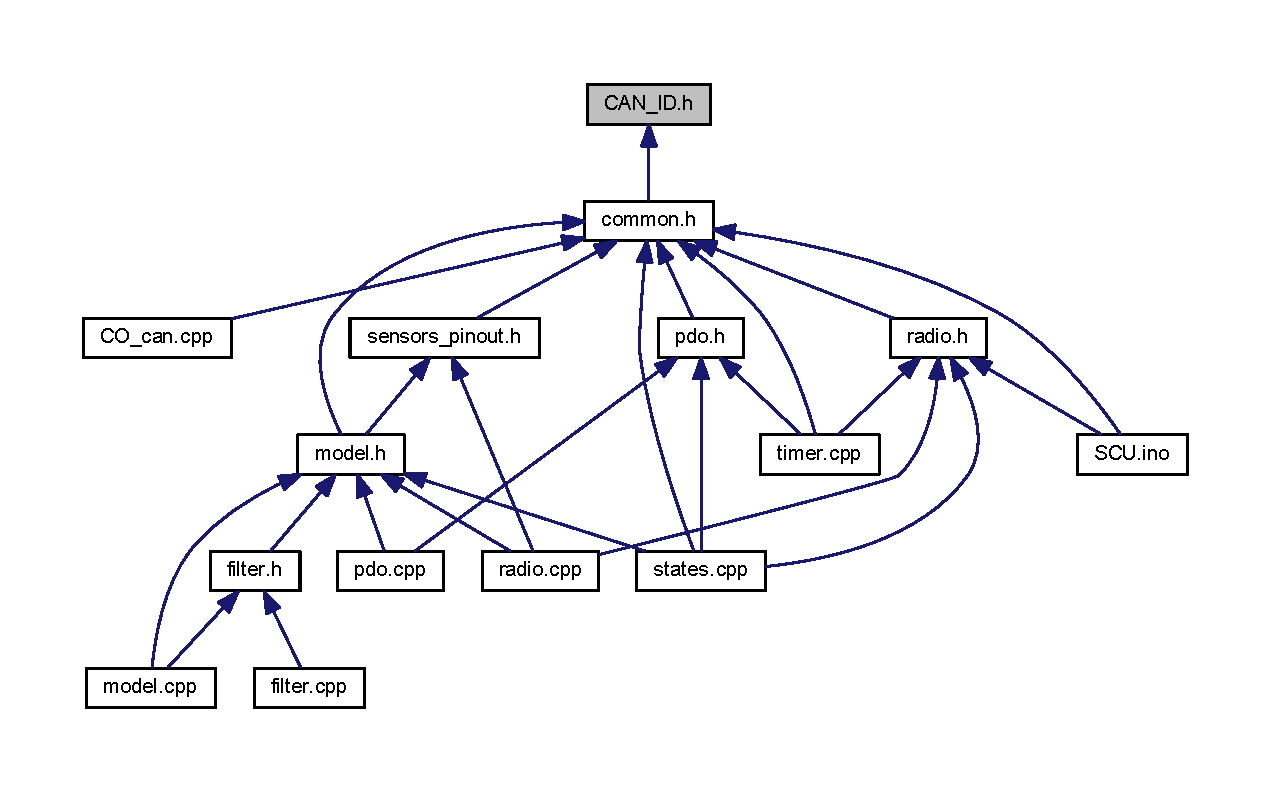
\includegraphics[width=350pt]{_c_a_n___i_d_8h__dep__incl}
\end{center}
\end{figure}
\subsection*{Macros}
\begin{DoxyCompactItemize}
\item 
\#define \mbox{\hyperlink{group___c_a_n___i_d_ga8d64b6b4c0f02ebded5440c6250e03b9}{S\+C\+U\+\_\+\+F\+R\+O\+N\+T\+A\+L\+\_\+\+N\+O\+D\+E\+\_\+\+ID}}~1
\begin{DoxyCompactList}\small\item\em Frontal S\+CU node ID on C\+AN servizi network. \end{DoxyCompactList}\item 
\#define \mbox{\hyperlink{group___c_a_n___i_d_ga5703fd8de5ab8d0dcedb561f2178829e}{V\+C\+U\+\_\+\+N\+O\+D\+E\+\_\+\+ID}}~2
\begin{DoxyCompactList}\small\item\em V\+CU node ID on C\+AN servizi network. \end{DoxyCompactList}\item 
\#define \mbox{\hyperlink{group___c_a_n___i_d_gab91968b64bc7fa886f6a6147d25d488b}{S\+C\+U\+\_\+\+R\+E\+A\+R\+\_\+\+N\+O\+D\+E\+\_\+\+ID}}~3
\begin{DoxyCompactList}\small\item\em Rear S\+CU node ID on C\+AN servizi network. \end{DoxyCompactList}\item 
\#define \mbox{\hyperlink{group___c_a_n___i_d_gaceef3f7366b39e88d89cb98ad8094c7b}{T\+C\+U\+\_\+\+N\+O\+D\+E\+\_\+\+ID}}~4
\begin{DoxyCompactList}\small\item\em T\+CU node ID on C\+AN servizi network. \end{DoxyCompactList}\end{DoxyCompactItemize}


\subsection{Detailed Description}
C\+AN servizi node\+I\+Ds module header. 

\begin{DoxyAuthor}{Author}
Arella Matteo ~\newline
 (mail\+: \href{mailto:arella.1646983@studenti.uniroma1.it}{\tt arella.\+1646983@studenti.\+uniroma1.\+it}) 
\end{DoxyAuthor}
\begin{DoxyDate}{Date}
2018 
\end{DoxyDate}

\hypertarget{_c_o__can_8cpp}{}\section{C\+O\+\_\+can.\+cpp File Reference}
\label{_c_o__can_8cpp}\index{C\+O\+\_\+can.\+cpp@{C\+O\+\_\+can.\+cpp}}


C\+A\+N\+Open main module implementation file.  


{\ttfamily \#include $<$due\+\_\+can.\+h$>$}\newline
{\ttfamily \#include \char`\"{}C\+O\+\_\+can.\+h\char`\"{}}\newline
{\ttfamily \#include \char`\"{}states.\+h\char`\"{}}\newline
{\ttfamily \#include \char`\"{}common.\+h\char`\"{}}\newline
Include dependency graph for C\+O\+\_\+can.\+cpp\+:\nopagebreak
\begin{figure}[H]
\begin{center}
\leavevmode
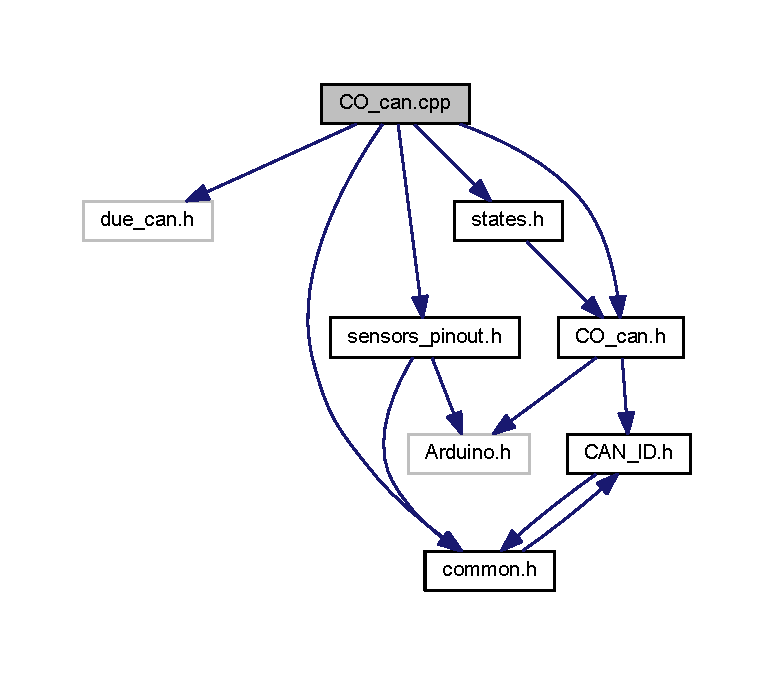
\includegraphics[width=330pt]{_c_o__can_8cpp__incl}
\end{center}
\end{figure}
\subsection*{Functions}
\begin{DoxyCompactItemize}
\item 
void \mbox{\hyperlink{group___c_a_n__network__module_ga44cc9b79c50c2c8eef6b98bac0d24dc9}{can\+Send}} (\mbox{\hyperlink{struct_message}{Message}} $\ast$m)
\begin{DoxyCompactList}\small\item\em This function send a C\+A\+Nopen message over C\+AN servizi network. \end{DoxyCompactList}\item 
void {\bfseries C\+A\+N\+\_\+general\+\_\+callback} (C\+A\+N\+\_\+\+F\+R\+A\+ME $\ast$frame)
\item 
void \mbox{\hyperlink{group___c_a_n__network__module_gaee4f95b5d4a9e9c330f3a9169464860a}{init\+C\+AN}} ()
\begin{DoxyCompactList}\small\item\em This function initialize C\+A\+N/\+C\+A\+Nopen interfaces and communication. \end{DoxyCompactList}\end{DoxyCompactItemize}


\subsection{Detailed Description}
C\+A\+N\+Open main module implementation file. 

\begin{DoxyAuthor}{Author}
Arella Matteo ~\newline
 (mail\+: \href{mailto:arella.1646983@studenti.uniroma1.it}{\tt arella.\+1646983@studenti.\+uniroma1.\+it}) 
\end{DoxyAuthor}
\begin{DoxyDate}{Date}
2018 
\end{DoxyDate}

\hypertarget{_c_o__can_8h}{}\section{C\+O\+\_\+can.\+h File Reference}
\label{_c_o__can_8h}\index{C\+O\+\_\+can.\+h@{C\+O\+\_\+can.\+h}}


C\+A\+N\+Open main module header.  


{\ttfamily \#include \char`\"{}C\+A\+N\+\_\+\+I\+D.\+h\char`\"{}}\newline
{\ttfamily \#include $<$Arduino.\+h$>$}\newline
Include dependency graph for C\+O\+\_\+can.\+h\+:\nopagebreak
\begin{figure}[H]
\begin{center}
\leavevmode
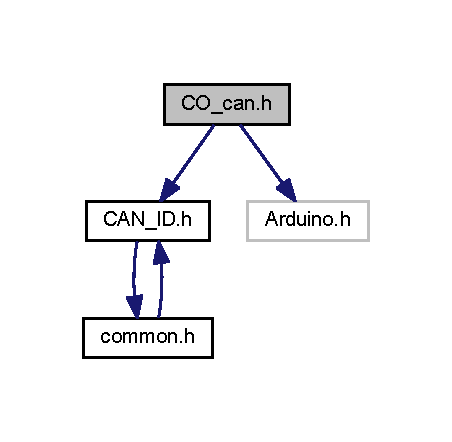
\includegraphics[width=217pt]{_c_o__can_8h__incl}
\end{center}
\end{figure}
This graph shows which files directly or indirectly include this file\+:\nopagebreak
\begin{figure}[H]
\begin{center}
\leavevmode
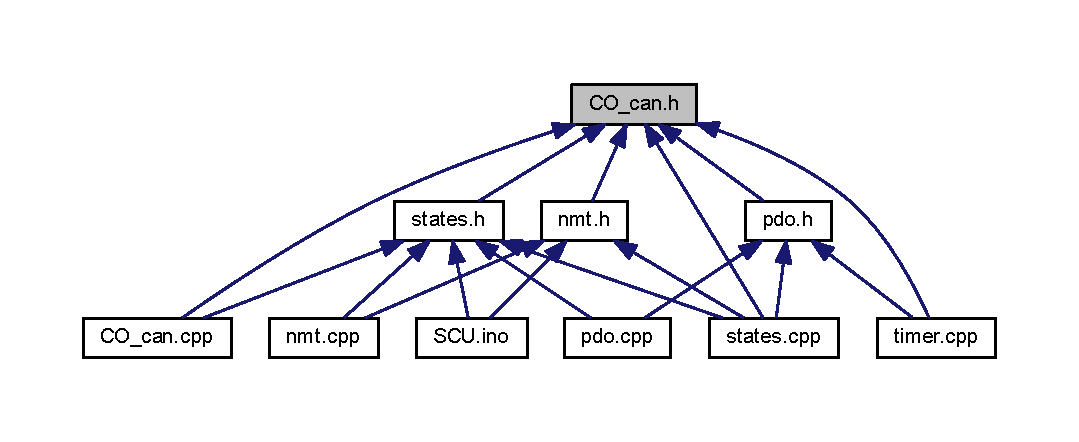
\includegraphics[width=350pt]{_c_o__can_8h__dep__incl}
\end{center}
\end{figure}
\subsection*{Classes}
\begin{DoxyCompactItemize}
\item 
struct \mbox{\hyperlink{struct_message}{Message}}
\begin{DoxyCompactList}\small\item\em C\+A\+Nopen message struct. \end{DoxyCompactList}\end{DoxyCompactItemize}
\subsection*{Macros}
\begin{DoxyCompactItemize}
\item 
\#define \mbox{\hyperlink{group___c_a_n__network__module_gaf21e24a8e9f1bf113b5efb16d5ab924b}{Message\+\_\+\+Initializer}}~\{0,0,\{0,0,0,0,0,0,0,0\}\}
\begin{DoxyCompactList}\small\item\em C\+A\+Nopen static message initializer. \end{DoxyCompactList}\end{DoxyCompactItemize}
\subsection*{Functions}
\begin{DoxyCompactItemize}
\item 
void \mbox{\hyperlink{group___c_a_n__network__module_gaee4f95b5d4a9e9c330f3a9169464860a}{init\+C\+AN}} ()
\begin{DoxyCompactList}\small\item\em This function initialize C\+A\+N/\+C\+A\+Nopen interfaces and communication. \end{DoxyCompactList}\item 
void \mbox{\hyperlink{group___c_a_n__network__module_ga44cc9b79c50c2c8eef6b98bac0d24dc9}{can\+Send}} (\mbox{\hyperlink{struct_message}{Message}} $\ast$m)
\begin{DoxyCompactList}\small\item\em This function send a C\+A\+Nopen message over C\+AN servizi network. \end{DoxyCompactList}\item 
uint8\+\_\+t \mbox{\hyperlink{group___c_a_n__network__module_gabf47bce7c4c8d2166fe3e25ac404d7c7}{get\+Node\+Id}} ()
\begin{DoxyCompactList}\small\item\em This function returns node ID into C\+AN servizi network. \end{DoxyCompactList}\item 
void \mbox{\hyperlink{group___c_a_n__network__module_ga9c3b7582805e01be4b88b6648b42837e}{set\+Node\+Id}} (uint8\+\_\+t \mbox{\hyperlink{group___c_a_n__network__module_gafe80bdea5c10c0d32fb3261a4e513fa9}{node\+Id}})
\begin{DoxyCompactList}\small\item\em This function sets node ID into C\+AN servizi network. \end{DoxyCompactList}\end{DoxyCompactItemize}


\subsection{Detailed Description}
C\+A\+N\+Open main module header. 

\begin{DoxyAuthor}{Author}
Arella Matteo ~\newline
 (mail\+: \href{mailto:arella.1646983@studenti.uniroma1.it}{\tt arella.\+1646983@studenti.\+uniroma1.\+it}) 
\end{DoxyAuthor}
\begin{DoxyDate}{Date}
2018 
\end{DoxyDate}

\hypertarget{common_8h}{}\section{common.\+h File Reference}
\label{common_8h}\index{common.\+h@{common.\+h}}


This file contains some common macro definitions for configuring main relevants parameters.  


{\ttfamily \#include \char`\"{}C\+A\+N\+\_\+\+I\+D.\+h\char`\"{}}\newline
Include dependency graph for common.\+h\+:\nopagebreak
\begin{figure}[H]
\begin{center}
\leavevmode
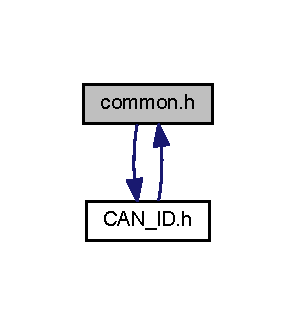
\includegraphics[width=142pt]{common_8h__incl}
\end{center}
\end{figure}
This graph shows which files directly or indirectly include this file\+:\nopagebreak
\begin{figure}[H]
\begin{center}
\leavevmode
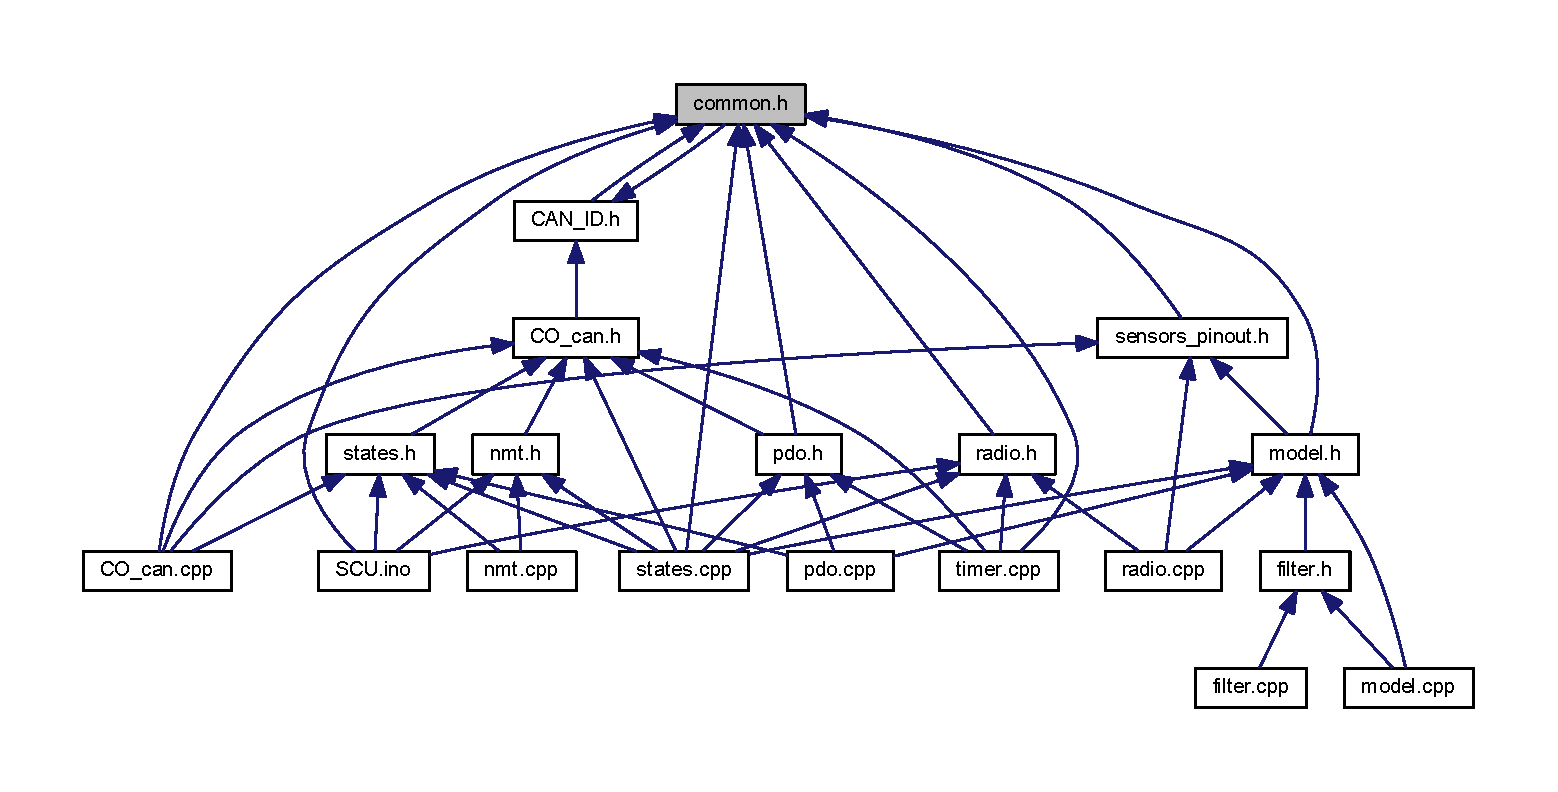
\includegraphics[width=350pt]{common_8h__dep__incl}
\end{center}
\end{figure}
\subsection*{Macros}
\begin{DoxyCompactItemize}
\item 
\#define \mbox{\hyperlink{group___common__defines__group_gaa75b7ce1cd135619656735399baf3768}{C\+A\+N\+\_\+\+B\+A\+U\+D\+R\+A\+TE}}~1000000
\begin{DoxyCompactList}\small\item\em C\+AN network baud rate \mbox{[} $bps$\mbox{]}. \end{DoxyCompactList}\item 
\#define \mbox{\hyperlink{group___common__defines__group_ga89f82a9d44beaa52b00c7245a50a105c}{S\+E\+R\+I\+A\+L\+\_\+\+B\+A\+U\+D\+R\+A\+TE}}~115200
\begin{DoxyCompactList}\small\item\em Serial U\+A\+RT baud rate \mbox{[} $bps$\mbox{]}. \end{DoxyCompactList}\item 
\#define \mbox{\hyperlink{group___common__defines__group_ga09c95853fd002fab968d94c5bc44e823}{T\+I\+M\+E\+\_\+\+S\+L\+O\+T\+\_\+\+P\+E\+R\+I\+OD}}~4000
\begin{DoxyCompactList}\small\item\em Timer period \mbox{[} $ms$\mbox{]}. \end{DoxyCompactList}\item 
\#define \mbox{\hyperlink{group___common__defines__group_ga599217205dc3092c26567a2bd868ef3a}{T\+I\+M\+ER}}~Timer3
\begin{DoxyCompactList}\small\item\em C\+A\+Nopen timer. \end{DoxyCompactList}\item 
\#define \mbox{\hyperlink{group___s_c_u__firmware__selection_gac03ca83c43ea664674af7e07a8da7879}{\+\_\+\+F\+R\+O\+N\+T\+A\+L\+\_\+}}
\begin{DoxyCompactList}\small\item\em Macro for selecting frontal S\+CU firmware. \end{DoxyCompactList}\item 
\#define \mbox{\hyperlink{group___s_c_u__firmware__selection_ga790010e78c29a0a2ffa3c09cc62d9f3d}{\+\_\+\+R\+E\+T\+R\+O\+\_\+}}
\begin{DoxyCompactList}\small\item\em Macro for selecting rear S\+CU firmware. \end{DoxyCompactList}\end{DoxyCompactItemize}


\subsection{Detailed Description}
This file contains some common macro definitions for configuring main relevants parameters. 

\begin{DoxyAuthor}{Author}
Arella Matteo ~\newline
 (mail\+: \href{mailto:arella.1646983@studenti.uniroma1.it}{\tt arella.\+1646983@studenti.\+uniroma1.\+it}) 
\end{DoxyAuthor}
\begin{DoxyDate}{Date}
2018 
\end{DoxyDate}

\hypertarget{def_8h}{}\section{def.\+h File Reference}
\label{def_8h}\index{def.\+h@{def.\+h}}


C\+A\+Nopen D\+S301 definitions.  


This graph shows which files directly or indirectly include this file\+:\nopagebreak
\begin{figure}[H]
\begin{center}
\leavevmode
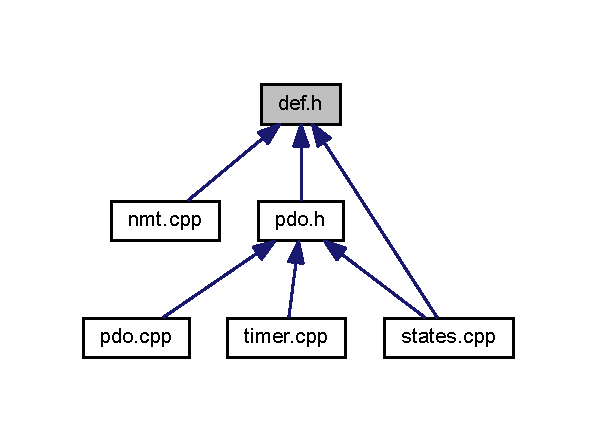
\includegraphics[width=287pt]{def_8h__dep__incl}
\end{center}
\end{figure}
\subsection*{Macros}
\begin{DoxyCompactItemize}
\item 
\#define \mbox{\hyperlink{group___c_a_nopen___func___codes_gaadbe0bb038acafa1c8adb0f98c870233}{N\+MT}}~0x0
\begin{DoxyCompactList}\small\item\em N\+MT function code. \end{DoxyCompactList}\item 
\#define \mbox{\hyperlink{group___c_a_nopen___func___codes_ga9ac82e856c7683e23553431e5224d5f4}{S\+Y\+NC}}~0x1
\begin{DoxyCompactList}\small\item\em S\+Y\+NC function code. \end{DoxyCompactList}\item 
\#define \mbox{\hyperlink{group___c_a_nopen___func___codes_ga5a63bf5566f66e30f56bc17eea0e5e4b}{T\+I\+M\+E\+\_\+\+S\+T\+A\+MP}}~0x2
\begin{DoxyCompactList}\small\item\em T\+I\+M\+E\+\_\+\+S\+T\+A\+MP function code. \end{DoxyCompactList}\item 
\#define \mbox{\hyperlink{group___c_a_nopen___func___codes_ga0a250614ba4dca3e87f768efcb58f238}{P\+D\+O1tx}}~0x3
\begin{DoxyCompactList}\small\item\em P\+D\+O1tx function code. \end{DoxyCompactList}\item 
\#define \mbox{\hyperlink{group___c_a_nopen___func___codes_ga17c7ee302d491b1ef74d2a4a795f82c6}{P\+D\+O1rx}}~0x4
\begin{DoxyCompactList}\small\item\em P\+D\+O1rx function code. \end{DoxyCompactList}\item 
\#define \mbox{\hyperlink{group___c_a_nopen___func___codes_ga67f4224b2c072a82b37a4835ca1c75e1}{P\+D\+O2tx}}~0x5
\begin{DoxyCompactList}\small\item\em P\+D\+O2tx function code. \end{DoxyCompactList}\item 
\#define \mbox{\hyperlink{group___c_a_nopen___func___codes_gab23848999420738438097816fee3f25d}{P\+D\+O2rx}}~0x6
\begin{DoxyCompactList}\small\item\em P\+D\+O2rx function code. \end{DoxyCompactList}\item 
\#define \mbox{\hyperlink{group___c_a_nopen___func___codes_ga00ef0f6ae698f9cb944b4302e66e6c83}{P\+D\+O3tx}}~0x7
\begin{DoxyCompactList}\small\item\em P\+D\+O3tx function code. \end{DoxyCompactList}\item 
\#define \mbox{\hyperlink{group___c_a_nopen___func___codes_ga239d135abea5ec798461cad43f9286b5}{P\+D\+O3rx}}~0x8
\begin{DoxyCompactList}\small\item\em P\+D\+O3rx function code. \end{DoxyCompactList}\item 
\#define \mbox{\hyperlink{group___c_a_nopen___func___codes_gabda4cc9ec44d1fc524bfdcae030df4be}{P\+D\+O4tx}}~0x9
\begin{DoxyCompactList}\small\item\em P\+D\+O4tx function code. \end{DoxyCompactList}\item 
\#define \mbox{\hyperlink{group___c_a_nopen___func___codes_ga282f714f745dd28e9a017044020aa3dc}{P\+D\+O4rx}}~0xA
\begin{DoxyCompactList}\small\item\em P\+D\+O4rx function code. \end{DoxyCompactList}\item 
\#define \mbox{\hyperlink{group___c_a_nopen___func___codes_ga74331e9b1d102bd0a3d5d9c1fc4f8212}{S\+D\+Otx}}~0xB
\begin{DoxyCompactList}\small\item\em S\+D\+Otx function code. \end{DoxyCompactList}\item 
\#define \mbox{\hyperlink{group___c_a_nopen___func___codes_ga44318f0cf5176db0eedd1c8519bd8f35}{S\+D\+Orx}}~0xC
\begin{DoxyCompactList}\small\item\em S\+D\+Orx function code. \end{DoxyCompactList}\item 
\#define \mbox{\hyperlink{group___c_a_nopen___func___codes_ga78d5d3f71db9f360c9e3d3953707b0c1}{N\+O\+D\+E\+\_\+\+G\+U\+A\+RD}}~0xE
\begin{DoxyCompactList}\small\item\em N\+O\+DE G\+U\+A\+RD function code. \end{DoxyCompactList}\item 
\#define \mbox{\hyperlink{group___c_a_nopen___func___codes_gaa09b700d4c6a1eac2a3068f446c397e2}{L\+SS}}~0xF
\begin{DoxyCompactList}\small\item\em L\+SS function code. \end{DoxyCompactList}\item 
\#define \mbox{\hyperlink{group___c_a_nopen___func___codes_gad4585eb139cc908014093ce9b81d0d51}{G\+E\+T\+\_\+\+F\+U\+N\+C\+\_\+\+C\+O\+DE}}(C\+O\+B\+\_\+\+ID)~(C\+O\+B\+\_\+\+ID $>$$>$ 7)
\begin{DoxyCompactList}\small\item\em Extract function code from C\+O\+B-\/\+ID. \end{DoxyCompactList}\item 
\#define \mbox{\hyperlink{group___c_a_nopen___func___codes_gade75ae84ef68190e83a60643194e91fd}{S\+E\+T\+\_\+\+F\+U\+N\+C\+\_\+\+C\+O\+DE}}(C\+O\+B\+\_\+\+ID)~(C\+O\+B\+\_\+\+ID $<$$<$ 7)
\begin{DoxyCompactList}\small\item\em Set function code to C\+O\+B-\/\+ID. \end{DoxyCompactList}\item 
\#define \mbox{\hyperlink{group___c_a_nopen___n_m_t__speficications_ga9654207fdc32413aa792c8a2dc9d414f}{N\+M\+T\+\_\+\+Start\+\_\+\+Node}}~0x01
\begin{DoxyCompactList}\small\item\em \textquotesingle{}go Operational\textquotesingle{} command specifier \end{DoxyCompactList}\item 
\#define \mbox{\hyperlink{group___c_a_nopen___n_m_t__speficications_ga7aae99c67e9ebd9491a246baf92570fa}{N\+M\+T\+\_\+\+Stop\+\_\+\+Node}}~0x02
\begin{DoxyCompactList}\small\item\em \textquotesingle{}stop Node\textquotesingle{} command specifier \end{DoxyCompactList}\item 
\#define \mbox{\hyperlink{group___c_a_nopen___n_m_t__speficications_gabdbbb7ecbe41058f60f684c10e07e08e}{N\+M\+T\+\_\+\+Enter\+\_\+\+Pre\+Operational}}~0x80
\begin{DoxyCompactList}\small\item\em \textquotesingle{}go Pre\+Operational\textquotesingle{} command specifier \end{DoxyCompactList}\item 
\#define \mbox{\hyperlink{group___c_a_nopen___n_m_t__speficications_gab349b5574a1ea67ff0ef76b9f9b6319e}{N\+M\+T\+\_\+\+Reset\+\_\+\+Node}}~0x81
\begin{DoxyCompactList}\small\item\em \textquotesingle{}reset Node\textquotesingle{} command specifier \end{DoxyCompactList}\item 
\#define \mbox{\hyperlink{group___c_a_nopen___n_m_t__speficications_gafd16bdbe636d7c761a9e015a7d7653ce}{N\+M\+T\+\_\+\+Reset\+\_\+\+Comunication}}~0x82
\begin{DoxyCompactList}\small\item\em \textquotesingle{}reset Communication\textquotesingle{} command specifier \end{DoxyCompactList}\end{DoxyCompactItemize}


\subsection{Detailed Description}
C\+A\+Nopen D\+S301 definitions. 

\begin{DoxyAuthor}{Author}
Arella Matteo ~\newline
 (mail\+: \href{mailto:arella.1646983@studenti.uniroma1.it}{\tt arella.\+1646983@studenti.\+uniroma1.\+it}) 
\end{DoxyAuthor}
\begin{DoxyDate}{Date}
2018 
\end{DoxyDate}

\hypertarget{filter_8cpp}{}\section{filter.\+cpp File Reference}
\label{filter_8cpp}\index{filter.\+cpp@{filter.\+cpp}}


Filter module implementation file.  


{\ttfamily \#include \char`\"{}filter.\+h\char`\"{}}\newline
Include dependency graph for filter.\+cpp\+:\nopagebreak
\begin{figure}[H]
\begin{center}
\leavevmode
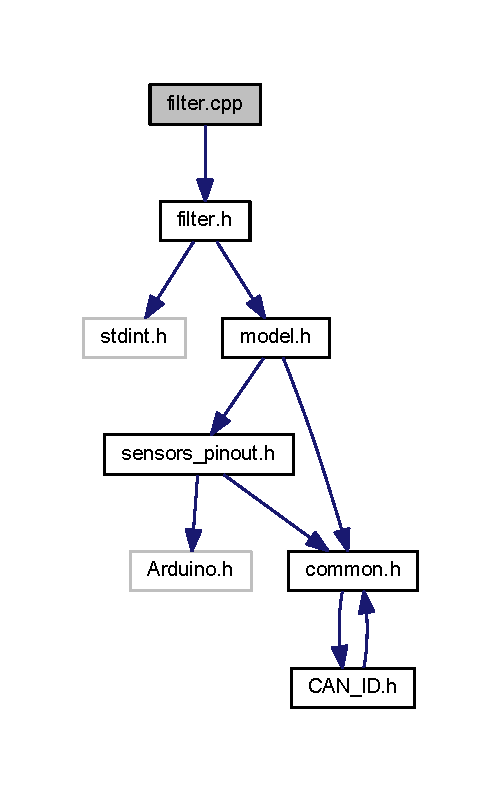
\includegraphics[width=241pt]{filter_8cpp__incl}
\end{center}
\end{figure}
\subsection*{Macros}
\begin{DoxyCompactItemize}
\item 
\#define \mbox{\hyperlink{group___filter__module__group_ga1646c21a91b653eeb516c9d508c1cab6}{U\+S\+E\+\_\+\+L\+O\+O\+P\+\_\+\+U\+N\+R\+O\+L\+L\+I\+NG}}~(1)
\begin{DoxyCompactList}\small\item\em Flag macro for using or not loop unrolling into filter function. \end{DoxyCompactList}\item 
\#define \mbox{\hyperlink{group___filter__module__group_gaa505bfa61df2c48cb76be56720dae3d1}{pos}}(x,  offset)~((x) $\ast$ offset)
\begin{DoxyCompactList}\small\item\em Buffer indexing macro. \end{DoxyCompactList}\end{DoxyCompactItemize}
\subsection*{Functions}
\begin{DoxyCompactItemize}
\item 
uint16\+\_\+t \mbox{\hyperlink{group___filter__module__group_ga676952eee893902e5a15b3f5adca1f86}{filter\+\_\+buffer}} (volatile uint16\+\_\+t $\ast$buffer, int size, unsigned offset)
\begin{DoxyCompactList}\small\item\em This function filters the input buffer with an average filter. \end{DoxyCompactList}\end{DoxyCompactItemize}


\subsection{Detailed Description}
Filter module implementation file. 

\begin{DoxyAuthor}{Author}
Arella Matteo ~\newline
 (mail\+: \href{mailto:arella.1646983@studenti.uniroma1.it}{\tt arella.\+1646983@studenti.\+uniroma1.\+it}) 
\end{DoxyAuthor}
\begin{DoxyDate}{Date}
2018 
\end{DoxyDate}

\hypertarget{filter_8h}{}\section{filter.\+h File Reference}
\label{filter_8h}\index{filter.\+h@{filter.\+h}}


Filter module header file.  


{\ttfamily \#include $<$stdint.\+h$>$}\newline
{\ttfamily \#include \char`\"{}model.\+h\char`\"{}}\newline
Include dependency graph for filter.\+h\+:\nopagebreak
\begin{figure}[H]
\begin{center}
\leavevmode
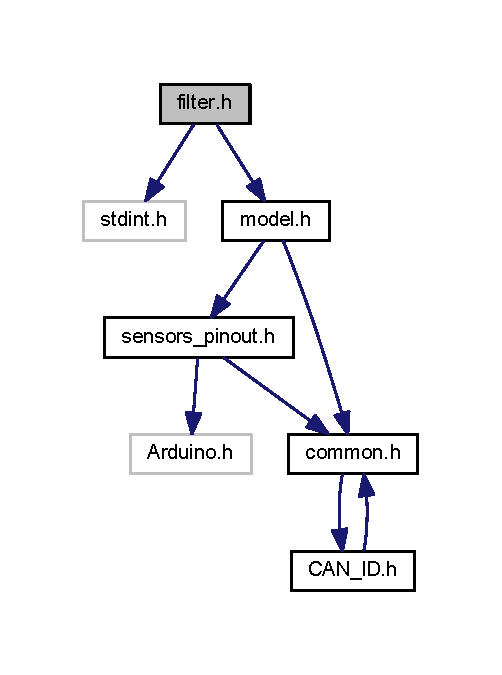
\includegraphics[width=241pt]{filter_8h__incl}
\end{center}
\end{figure}
This graph shows which files directly or indirectly include this file\+:\nopagebreak
\begin{figure}[H]
\begin{center}
\leavevmode
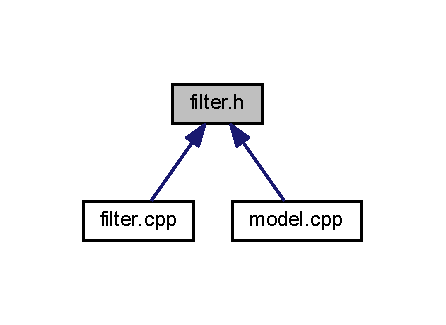
\includegraphics[width=214pt]{filter_8h__dep__incl}
\end{center}
\end{figure}
\subsection*{Functions}
\begin{DoxyCompactItemize}
\item 
uint16\+\_\+t \mbox{\hyperlink{group___filter__module__group_ga676952eee893902e5a15b3f5adca1f86}{filter\+\_\+buffer}} (volatile uint16\+\_\+t $\ast$buffer, int size, unsigned offset)
\begin{DoxyCompactList}\small\item\em This function filters the input buffer with an average filter. \end{DoxyCompactList}\end{DoxyCompactItemize}


\subsection{Detailed Description}
Filter module header file. 

\begin{DoxyAuthor}{Author}
Arella Matteo ~\newline
 (mail\+: \href{mailto:arella.1646983@studenti.uniroma1.it}{\tt arella.\+1646983@studenti.\+uniroma1.\+it}) 
\end{DoxyAuthor}
\begin{DoxyDate}{Date}
2018 
\end{DoxyDate}

\hypertarget{model_8cpp}{}\section{model.\+cpp File Reference}
\label{model_8cpp}\index{model.\+cpp@{model.\+cpp}}


Board model implementation file.  


{\ttfamily \#include \char`\"{}model.\+h\char`\"{}}\newline
{\ttfamily \#include \char`\"{}filter.\+h\char`\"{}}\newline
Include dependency graph for model.\+cpp\+:\nopagebreak
\begin{figure}[H]
\begin{center}
\leavevmode
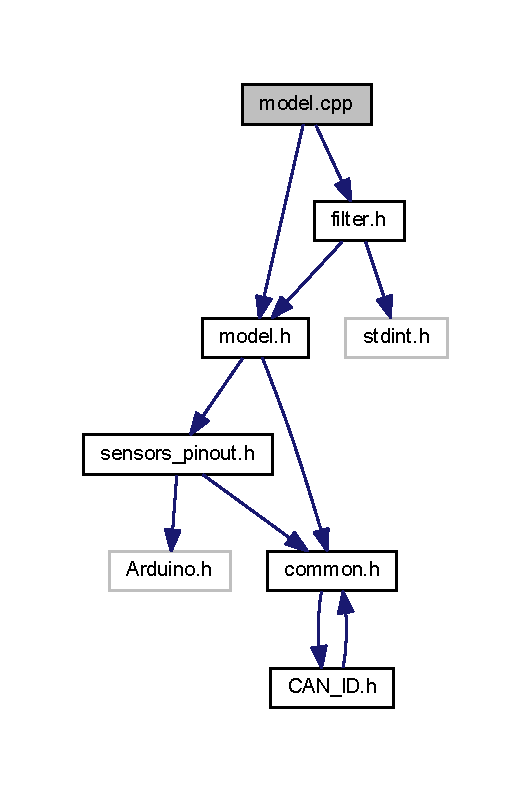
\includegraphics[width=255pt]{model_8cpp__incl}
\end{center}
\end{figure}
\subsection*{Macros}
\begin{DoxyCompactItemize}
\item 
\#define \mbox{\hyperlink{group___board__model__group_ga602abb8ec84dcb3b6f854a738310ea46}{A\+D\+C\+\_\+\+B\+U\+F\+F\+E\+R\+\_\+\+S\+I\+ZE}}~128
\begin{DoxyCompactList}\small\item\em Size (bytes) of buffer for store each A\+DC channel data with D\+MA. \end{DoxyCompactList}\item 
\#define \mbox{\hyperlink{group___board__model__group_gaabe0f927d44a09f458bd5fe5ab4e2f7f}{B\+U\+F\+F\+E\+RS}}~4
\begin{DoxyCompactList}\small\item\em Number of D\+MA buffers. \end{DoxyCompactList}\item 
\#define \mbox{\hyperlink{group___board__model__group_gaf0098a1eafb8a60a1c65773e1064d595}{A\+D\+C\+\_\+\+M\+IN}}~0
\begin{DoxyCompactList}\small\item\em A\+DC lower bound value. \end{DoxyCompactList}\item 
\#define \mbox{\hyperlink{group___board__model__group_ga555a695bf58df062dc03f0e892d95cd7}{A\+D\+C\+\_\+\+M\+AX}}~4095
\begin{DoxyCompactList}\small\item\em A\+DC upper bound value. \end{DoxyCompactList}\item 
\#define \mbox{\hyperlink{group___board__model__group_ga6741cba3daf129b6f73eed1b1db09519}{T\+P\+S1\+\_\+\+U\+P\+P\+E\+R\+\_\+\+B\+O\+U\+ND}}~2482
\begin{DoxyCompactList}\small\item\em First A\+P\+PS max output voltage (2V) \end{DoxyCompactList}\item 
\#define \mbox{\hyperlink{group___board__model__group_ga9c9aa914f6b372d9ef3f15ce4108da6a}{T\+P\+S1\+\_\+\+L\+O\+W\+E\+R\+\_\+\+B\+O\+U\+ND}}~993
\begin{DoxyCompactList}\small\item\em First A\+P\+PS min output voltage (0.\+8V) \end{DoxyCompactList}\item 
\#define \mbox{\hyperlink{group___board__model__group_gac8be8d89c699c40b79d04c0fdf6238f4}{T\+P\+S2\+\_\+\+U\+P\+P\+E\+R\+\_\+\+B\+O\+U\+ND}}~1241
\begin{DoxyCompactList}\small\item\em Second A\+P\+PS max output voltage (1V) \end{DoxyCompactList}\item 
\#define \mbox{\hyperlink{group___board__model__group_gadfcc723e175ac44e73e38407299ac875}{T\+P\+S2\+\_\+\+L\+O\+W\+E\+R\+\_\+\+B\+O\+U\+ND}}~497
\begin{DoxyCompactList}\small\item\em Second A\+P\+PS min output voltage (0.\+4V) \end{DoxyCompactList}\item 
\#define \mbox{\hyperlink{group___board__model__group_ga891de03ab9e1bd9a92ffffe69a1b10ca}{B\+R\+A\+K\+E\+\_\+\+U\+P\+P\+E\+R\+\_\+\+B\+O\+U\+ND}}~0
\begin{DoxyCompactList}\small\item\em Brake sensor max output voltage (T\+O\+DO\+: check Voutmax) \end{DoxyCompactList}\item 
\#define \mbox{\hyperlink{group___board__model__group_ga0aed20cafcc206360abda47b125432c7}{B\+R\+A\+K\+E\+\_\+\+L\+O\+W\+E\+R\+\_\+\+B\+O\+U\+ND}}~\mbox{\hyperlink{group___board__model__group_ga555a695bf58df062dc03f0e892d95cd7}{A\+D\+C\+\_\+\+M\+AX}}
\begin{DoxyCompactList}\small\item\em Brake sensor min output voltage (T\+O\+DO\+: check Voutmin) \end{DoxyCompactList}\item 
\#define \mbox{\hyperlink{group___board__model__group_ga2445bb784c1bcde9b88c5f81fc814055}{S\+U\+S\+P\+E\+N\+S\+I\+O\+N\+S\+\_\+\+M\+IN}}~0
\begin{DoxyCompactList}\small\item\em Minimum suspension stroke \mbox{[} $mm$\mbox{]}. \end{DoxyCompactList}\item 
\#define \mbox{\hyperlink{group___board__model__group_gaf662e0e156dae3a519648a2f10fa3635}{S\+U\+S\+P\+E\+N\+S\+I\+O\+N\+S\+\_\+\+A\+D\+C\+\_\+\+M\+AX}}~\mbox{\hyperlink{group___board__model__group_ga555a695bf58df062dc03f0e892d95cd7}{A\+D\+C\+\_\+\+M\+AX}}
\begin{DoxyCompactList}\small\item\em Maximum suspension sensor $V_{OUT}$. \end{DoxyCompactList}\item 
\#define \mbox{\hyperlink{group___board__model__group_gadad409d745f70ca3c312ca3914a43822}{S\+U\+S\+P\+\_\+\+S\+T\+R\+O\+K\+E\+\_\+\+N\+O\+R\+M\+A\+L\+I\+ZE}}~(\mbox{\hyperlink{group___board__model__group_gafd34b4e5a1067ffe9bfb1cb18b5973e6}{S\+U\+S\+P\+\_\+\+S\+T\+R\+O\+K\+E\+\_\+\+E\+X\+T\+E\+N\+S\+I\+ON}} / \mbox{\hyperlink{group___board__model__group_gaf662e0e156dae3a519648a2f10fa3635}{S\+U\+S\+P\+E\+N\+S\+I\+O\+N\+S\+\_\+\+A\+D\+C\+\_\+\+M\+AX}})
\begin{DoxyCompactList}\small\item\em Suspension stroke voltage normalizer. \end{DoxyCompactList}\item 
\#define \mbox{\hyperlink{group___board__model__group_gab4fd15d90627818134453e8399055f7d}{C\+O\+G\+S\+\_\+\+N\+U\+M\+B\+ER}}~30.\+0d
\begin{DoxyCompactList}\small\item\em Number of phonic wheel\textquotesingle{}s cogs. \end{DoxyCompactList}\item 
\#define \mbox{\hyperlink{group___board__model__group_ga579e1065b83e6aef14ce222295f8b7eb}{N\+O\+R\+M\+A\+L\+I\+Z\+E\+\_\+\+R\+PM}}~1000000.\+0d
\begin{DoxyCompactList}\small\item\em Normalize time domain \mbox{[} $\mu s$\mbox{]}. \end{DoxyCompactList}\item 
\#define \mbox{\hyperlink{group___board__model__group_gafc05771487f188ffa40b6620afc1a9bc}{R\+P\+M\+\_\+\+M\+IN}}~10
\begin{DoxyCompactList}\small\item\em Rpm lower bound under that rpm are forced to zero. \end{DoxyCompactList}\item 
\#define \mbox{\hyperlink{group___board__model__group_gaa8634c7b040cfe3e016765395a38efa3}{A\+C\+C\+E\+L\+E\+R\+O\+M\+E\+T\+E\+R\+\_\+\+M\+A\+X\+\_\+G}}~5.\+0d
\begin{DoxyCompactList}\small\item\em Accelerometer sensor maximum value \mbox{[} $m/s^{2}$\mbox{]}. \end{DoxyCompactList}\item 
\#define \mbox{\hyperlink{group___board__model__group_ga5b18e6cd4163d6006ddf3c1f8a1e2a72}{A\+C\+C\+E\+L\+E\+R\+O\+M\+E\+T\+E\+R\+\_\+\+N\+O\+R\+M\+A\+L\+I\+ZE}}~2.\+0d $\ast$ A\+C\+C\+E\+L\+E\+R\+O\+M\+E\+T\+E\+R\+\_\+\+M\+A\+X\+\_\+\+G / A\+D\+C\+\_\+\+M\+AX
\begin{DoxyCompactList}\small\item\em Accelerometer sensor voltage normalizer. \end{DoxyCompactList}\item 
\#define \mbox{\hyperlink{group___board__model__group_ga3e1022cd2e2154437b583f7ff83f2960}{A\+P\+P\+S\+\_\+\+P\+L\+A\+U\+S\+\_\+\+R\+A\+N\+GE}}~10
\begin{DoxyCompactList}\small\item\em Maximum percentage deviation of pedal travel between two A\+P\+PS. \end{DoxyCompactList}\item 
\#define \mbox{\hyperlink{group___board__model__group_ga99f732ac210a4d6b6635ed58681d3d71}{S\+C\+U\+\_\+\+F\+R\+O\+N\+T\+A\+L\+\_\+\+A\+D\+C\+\_\+\+C\+H\+A\+N\+N\+E\+LS}}~5
\begin{DoxyCompactList}\small\item\em Number of A\+DC channels used in frontal S\+CU board. \end{DoxyCompactList}\item 
\#define \mbox{\hyperlink{group___board__model__group_ga1b36d02d5fef3342ea7159722fa50ff3}{S\+C\+U\+\_\+\+F\+R\+O\+N\+T\+A\+L\+\_\+\+A\+D\+C\+\_\+\+C\+H\+A\+N\+N\+E\+L\+S\+\_\+\+L\+I\+ST}}~\mbox{\hyperlink{group___board__pinout__group_ga99b2a7dadaf495e3c559a46440f9141f}{T\+P\+S1\+\_\+\+A\+D\+C\+\_\+\+C\+H\+A\+N\+\_\+\+N\+UM}} $\vert$ \mbox{\hyperlink{group___board__pinout__group_ga4cecb8c10512873904099a1a88d69ed3}{T\+P\+S2\+\_\+\+A\+D\+C\+\_\+\+C\+H\+A\+N\+\_\+\+N\+UM}} $\vert$ \mbox{\hyperlink{group___board__pinout__group_ga310547321c4a016c4ad19922920fadfd}{B\+R\+A\+K\+E\+\_\+\+A\+D\+C\+\_\+\+C\+H\+A\+N\+\_\+\+N\+UM}} $\vert$ \mbox{\hyperlink{group___board__pinout__group_gab536d8e8e876dfd8764cc1d31620803a}{F\+R\+\_\+\+S\+X\+\_\+\+A\+D\+C\+\_\+\+C\+H\+A\+N\+\_\+\+N\+UM}} $\vert$ \mbox{\hyperlink{group___board__pinout__group_ga9d0085cf869db954c00e9c13d9661d51}{F\+R\+\_\+\+D\+X\+\_\+\+A\+D\+C\+\_\+\+C\+H\+A\+N\+\_\+\+N\+UM}}
\begin{DoxyCompactList}\small\item\em List of A\+DC channels dedicated to each IO port in frontal S\+CU board. \end{DoxyCompactList}\item 
\#define \mbox{\hyperlink{group___board__model__group_gadedc78ae5ed236e74a4e12c031209d29}{S\+C\+U\+\_\+\+R\+E\+T\+R\+O\+\_\+\+A\+D\+C\+\_\+\+C\+H\+A\+N\+N\+E\+LS}}~4
\begin{DoxyCompactList}\small\item\em Number of A\+DC channels used in rear S\+CU board. \end{DoxyCompactList}\item 
\#define \mbox{\hyperlink{group___board__model__group_ga5190c5da456959fb6c7132518a51f12f}{S\+C\+U\+\_\+\+R\+E\+T\+R\+O\+\_\+\+A\+D\+C\+\_\+\+C\+H\+A\+N\+N\+E\+L\+S\+\_\+\+L\+I\+ST}}~A\+C\+C\+\_\+\+X\+\_\+\+A\+D\+C\+\_\+\+C\+H\+A\+N\+\_\+\+N\+UM $\vert$ A\+C\+C\+\_\+\+Z\+\_\+\+A\+D\+C\+\_\+\+C\+H\+A\+N\+\_\+\+N\+UM $\vert$ R\+T\+\_\+\+S\+X\+\_\+\+A\+D\+C\+\_\+\+C\+H\+A\+N\+\_\+\+N\+UM $\vert$ R\+T\+\_\+\+D\+X\+\_\+\+A\+D\+C\+\_\+\+C\+H\+A\+N\+\_\+\+N\+UM
\begin{DoxyCompactList}\small\item\em List of A\+DC channels dedicated to each IO port in retro S\+CU board. \end{DoxyCompactList}\item 
\#define \mbox{\hyperlink{group___board__model__group_ga7ce02d79fba23321a377a26a963e2bdf}{T\+P\+S1\+\_\+\+A\+D\+C\+\_\+\+O\+F\+F\+S\+ET}}~0
\begin{DoxyCompactList}\small\item\em Offset from D\+MA buffer. \end{DoxyCompactList}\item 
\#define \mbox{\hyperlink{group___board__model__group_ga24019e59e805c7acf8f816e141d3d689}{T\+P\+S2\+\_\+\+A\+D\+C\+\_\+\+O\+F\+F\+S\+ET}}~1
\begin{DoxyCompactList}\small\item\em Offset from D\+MA buffer. \end{DoxyCompactList}\item 
\#define \mbox{\hyperlink{group___board__model__group_gade98eccd60c9b68cde78ca4c0009a84c}{B\+R\+A\+K\+E\+\_\+\+A\+D\+C\+\_\+\+O\+F\+F\+S\+ET}}~2
\begin{DoxyCompactList}\small\item\em Offset from D\+MA buffer. \end{DoxyCompactList}\item 
\#define \mbox{\hyperlink{group___board__model__group_gad2f9dcce783b10da16c47480a6ee69c2}{F\+R\+\_\+\+S\+X\+\_\+\+A\+D\+C\+\_\+\+O\+F\+F\+S\+ET}}~3
\begin{DoxyCompactList}\small\item\em Offset from D\+MA buffer. \end{DoxyCompactList}\item 
\#define \mbox{\hyperlink{group___board__model__group_gae4816219f422d1c427c5f1ee5464ff54}{F\+R\+\_\+\+D\+X\+\_\+\+A\+D\+C\+\_\+\+O\+F\+F\+S\+ET}}~4
\begin{DoxyCompactList}\small\item\em Offset from D\+MA buffer. \end{DoxyCompactList}\item 
\#define \mbox{\hyperlink{group___board__model__group_ga88bac7626143add751ec06d0a6f4f969}{A\+C\+C\+\_\+\+X\+\_\+\+A\+D\+C\+\_\+\+O\+F\+F\+S\+ET}}~0
\begin{DoxyCompactList}\small\item\em Offset from D\+MA buffer. \end{DoxyCompactList}\item 
\#define \mbox{\hyperlink{group___board__model__group_ga9712a0d42e65367ee89093f6153ed0f5}{A\+C\+C\+\_\+\+Z\+\_\+\+A\+D\+C\+\_\+\+O\+F\+F\+S\+ET}}~1
\begin{DoxyCompactList}\small\item\em Offset from D\+MA buffer. \end{DoxyCompactList}\item 
\#define \mbox{\hyperlink{group___board__model__group_gaf318359d2387fb8fb87719ef9575b4b5}{R\+T\+\_\+\+S\+X\+\_\+\+A\+D\+C\+\_\+\+O\+F\+F\+S\+ET}}~2
\begin{DoxyCompactList}\small\item\em Offset from D\+MA buffer. \end{DoxyCompactList}\item 
\#define \mbox{\hyperlink{group___board__model__group_gae702ce1b301d77d1f4e9b28d8ba12972}{R\+T\+\_\+\+D\+X\+\_\+\+A\+D\+C\+\_\+\+O\+F\+F\+S\+ET}}~3
\begin{DoxyCompactList}\small\item\em Offset from D\+MA buffer. \end{DoxyCompactList}\item 
\#define \mbox{\hyperlink{group___board__model__group_gaf7b7dc9a200cb1404c280bd500fd1551}{B\+U\+F\+F\+E\+R\+\_\+\+L\+E\+N\+G\+TH}}~\mbox{\hyperlink{group___board__model__group_ga602abb8ec84dcb3b6f854a738310ea46}{A\+D\+C\+\_\+\+B\+U\+F\+F\+E\+R\+\_\+\+S\+I\+ZE}} $\ast$ A\+D\+C\+\_\+\+C\+H\+A\+N\+N\+E\+LS
\begin{DoxyCompactList}\small\item\em Length, in bytes, of each D\+MA buffer. \end{DoxyCompactList}\end{DoxyCompactItemize}
\subsection*{Functions}
\begin{DoxyCompactItemize}
\item 
void \mbox{\hyperlink{group___board__model__group_ga40f87aeb451c092cf21baf57defc516e}{fr\+\_\+sx\+\_\+pulse}} ()
\begin{DoxyCompactList}\small\item\em E\+X\+TI I\+RQ handler. External interrupt handler executed when frontal left wheel encoder finds a hole into phonic wheel. \end{DoxyCompactList}\item 
void \mbox{\hyperlink{group___board__model__group_ga809e754563f2877e3264fd49483ceac9}{fr\+\_\+dx\+\_\+pulse}} ()
\begin{DoxyCompactList}\small\item\em E\+X\+TI I\+RQ handler. External interrupt handler executed when frontal right wheel encoder finds a hole into phonic wheel. \end{DoxyCompactList}\item 
volatile uint16\+\_\+t \mbox{\hyperlink{group___board__model__group_ga77eb7343baa6cbfd81673dcbd03ac125}{get\+\_\+fr\+\_\+sx\+\_\+rpm}} ()
\begin{DoxyCompactList}\small\item\em If rpm value is lower than \mbox{\hyperlink{group___board__model__group_gafc05771487f188ffa40b6620afc1a9bc}{R\+P\+M\+\_\+\+M\+IN}}, output is forced to zero. \end{DoxyCompactList}\item 
volatile uint16\+\_\+t \mbox{\hyperlink{group___board__model__group_ga3f71b1feaa9b3356080597de5de12f7b}{get\+\_\+fr\+\_\+dx\+\_\+rpm}} ()
\begin{DoxyCompactList}\small\item\em If rpm value is lower than \mbox{\hyperlink{group___board__model__group_gafc05771487f188ffa40b6620afc1a9bc}{R\+P\+M\+\_\+\+M\+IN}}, output is forced to zero. \end{DoxyCompactList}\item 
void \mbox{\hyperlink{group___board__model__group_gaedc241164d501dcbc52cde232333c9cf}{A\+D\+C\+\_\+\+Handler}} ()
\begin{DoxyCompactList}\small\item\em A\+DC I\+RQ handler. When A\+DC buffer is filled D\+MA pointer is linked to next buffer available. Then acquired data are filtered. \end{DoxyCompactList}\item 
void \mbox{\hyperlink{group___board__model__group_gace5a444da39d4366693503c53f0841c2}{model\+\_\+init}} ()
\begin{DoxyCompactList}\small\item\em This function initializes hardware board. \end{DoxyCompactList}\end{DoxyCompactItemize}
\subsection*{Variables}
\begin{DoxyCompactItemize}
\item 
volatile int \mbox{\hyperlink{group___board__model__group_gad2658b77f345b15c03759c02d1ba0e81}{bufn}}
\begin{DoxyCompactList}\small\item\em D\+MA buffer pointer. \end{DoxyCompactList}\item 
volatile int \mbox{\hyperlink{group___board__model__group_gafef4d6ed48b3edc5f7a74defba82e7d8}{obufn}}
\begin{DoxyCompactList}\small\item\em D\+MA buffer pointer. \end{DoxyCompactList}\item 
volatile uint16\+\_\+t \mbox{\hyperlink{group___board__model__group_ga2bab0e665606eb5a547deb0d23446f41}{buf}} \mbox{[}\mbox{\hyperlink{group___board__model__group_gaabe0f927d44a09f458bd5fe5ab4e2f7f}{B\+U\+F\+F\+E\+RS}}\mbox{]}\mbox{[}\mbox{\hyperlink{group___board__model__group_gaf7b7dc9a200cb1404c280bd500fd1551}{B\+U\+F\+F\+E\+R\+\_\+\+L\+E\+N\+G\+TH}}\mbox{]}
\begin{DoxyCompactList}\small\item\em D\+MA buffers\+: \mbox{\hyperlink{group___board__model__group_gaabe0f927d44a09f458bd5fe5ab4e2f7f}{B\+U\+F\+F\+E\+RS}} number of buffers each of \mbox{\hyperlink{group___board__model__group_gaf7b7dc9a200cb1404c280bd500fd1551}{B\+U\+F\+F\+E\+R\+\_\+\+L\+E\+N\+G\+TH}} size; D\+MA is configured in cyclic mode\+: after one of \mbox{\hyperlink{group___board__model__group_gaabe0f927d44a09f458bd5fe5ab4e2f7f}{B\+U\+F\+F\+E\+RS}} is filled then D\+MA transfer head moves to next buffer in circular indexing. \end{DoxyCompactList}\item 
volatile uint16\+\_\+t \mbox{\hyperlink{group___board__model__group_ga3d6043851868b7da3c1d6381f835a559}{tps1\+\_\+value}} = 0
\begin{DoxyCompactList}\small\item\em First A\+P\+PS value retrieved directly by analog tps1 signal (\mbox{\hyperlink{group___board__pinout__group_gae9aa914854f611488701c96a330b0bd4}{T\+P\+S1\+\_\+\+P\+IN}}) and filtered after D\+MA buffer is filled entirely. \end{DoxyCompactList}\item 
volatile uint16\+\_\+t \mbox{\hyperlink{group___board__model__group_gaa8a9b03858f40eadfd5d3d6c3e266834}{tps2\+\_\+value}} = 0
\begin{DoxyCompactList}\small\item\em Second A\+P\+PS value retrieved directly by analog tps2 signal (\mbox{\hyperlink{group___board__pinout__group_gab13a816bae3ca994897fc6f1cb590a67}{T\+P\+S2\+\_\+\+P\+IN}}) and filtered after D\+MA buffer is filled entirely. \end{DoxyCompactList}\item 
volatile uint16\+\_\+t \mbox{\hyperlink{group___board__model__group_gad7966e70fb4bebc6947eb3fbb059a3c9}{brake\+\_\+value}} = 0
\begin{DoxyCompactList}\small\item\em Brake pedal position sensor value retrieved directly by analog brake signal (\mbox{\hyperlink{group___board__pinout__group_gad632b56bf4c6259a390c3db91607078e}{B\+R\+A\+K\+E\+\_\+\+P\+IN}}) and filtered after D\+MA buffer is filled entirely. \end{DoxyCompactList}\item 
volatile uint16\+\_\+t \mbox{\hyperlink{group___board__model__group_gaf1d46fb483b2a63c3da25c11688af7c4}{tps1\+\_\+max}} = \mbox{\hyperlink{group___board__model__group_ga6741cba3daf129b6f73eed1b1db09519}{T\+P\+S1\+\_\+\+U\+P\+P\+E\+R\+\_\+\+B\+O\+U\+ND}}
\begin{DoxyCompactList}\small\item\em First A\+P\+PS max output voltage (equals to \mbox{\hyperlink{group___board__model__group_ga6741cba3daf129b6f73eed1b1db09519}{T\+P\+S1\+\_\+\+U\+P\+P\+E\+R\+\_\+\+B\+O\+U\+ND}}) \end{DoxyCompactList}\item 
volatile uint16\+\_\+t \mbox{\hyperlink{group___board__model__group_gab7d6ace1f9174e39ed6abbe4aaceb7f4}{tps1\+\_\+min}} = \mbox{\hyperlink{group___board__model__group_ga9c9aa914f6b372d9ef3f15ce4108da6a}{T\+P\+S1\+\_\+\+L\+O\+W\+E\+R\+\_\+\+B\+O\+U\+ND}}
\begin{DoxyCompactList}\small\item\em First A\+P\+PS min output voltage (equals to \mbox{\hyperlink{group___board__model__group_ga9c9aa914f6b372d9ef3f15ce4108da6a}{T\+P\+S1\+\_\+\+L\+O\+W\+E\+R\+\_\+\+B\+O\+U\+ND}}) \end{DoxyCompactList}\item 
volatile uint16\+\_\+t \mbox{\hyperlink{group___board__model__group_ga53381436ea8db96c356db8b305bec988}{tps2\+\_\+max}} = \mbox{\hyperlink{group___board__model__group_gac8be8d89c699c40b79d04c0fdf6238f4}{T\+P\+S2\+\_\+\+U\+P\+P\+E\+R\+\_\+\+B\+O\+U\+ND}}
\begin{DoxyCompactList}\small\item\em Second A\+P\+PS max output voltage (equals to \mbox{\hyperlink{group___board__model__group_gac8be8d89c699c40b79d04c0fdf6238f4}{T\+P\+S2\+\_\+\+U\+P\+P\+E\+R\+\_\+\+B\+O\+U\+ND}}) \end{DoxyCompactList}\item 
volatile uint16\+\_\+t \mbox{\hyperlink{group___board__model__group_ga4e7715668b19738d8bfd47f2420aff02}{tps2\+\_\+min}} = \mbox{\hyperlink{group___board__model__group_gadfcc723e175ac44e73e38407299ac875}{T\+P\+S2\+\_\+\+L\+O\+W\+E\+R\+\_\+\+B\+O\+U\+ND}}
\begin{DoxyCompactList}\small\item\em Second A\+P\+PS min output voltage (equals to \mbox{\hyperlink{group___board__model__group_gadfcc723e175ac44e73e38407299ac875}{T\+P\+S2\+\_\+\+L\+O\+W\+E\+R\+\_\+\+B\+O\+U\+ND}}) \end{DoxyCompactList}\item 
volatile uint16\+\_\+t \mbox{\hyperlink{group___board__model__group_ga744857a9bc060647cfc4ad47017c5bee}{brake\+\_\+max}} = \mbox{\hyperlink{group___board__model__group_ga891de03ab9e1bd9a92ffffe69a1b10ca}{B\+R\+A\+K\+E\+\_\+\+U\+P\+P\+E\+R\+\_\+\+B\+O\+U\+ND}}
\begin{DoxyCompactList}\small\item\em Brake sensor max output voltage (equals to \mbox{\hyperlink{group___board__model__group_ga891de03ab9e1bd9a92ffffe69a1b10ca}{B\+R\+A\+K\+E\+\_\+\+U\+P\+P\+E\+R\+\_\+\+B\+O\+U\+ND}}) \end{DoxyCompactList}\item 
volatile uint16\+\_\+t \mbox{\hyperlink{group___board__model__group_ga779ee9b904930e3cfb165e70edfecd02}{brake\+\_\+min}} = \mbox{\hyperlink{group___board__model__group_ga0aed20cafcc206360abda47b125432c7}{B\+R\+A\+K\+E\+\_\+\+L\+O\+W\+E\+R\+\_\+\+B\+O\+U\+ND}}
\begin{DoxyCompactList}\small\item\em Brake sensor min output voltage (equals to \mbox{\hyperlink{group___board__model__group_ga0aed20cafcc206360abda47b125432c7}{B\+R\+A\+K\+E\+\_\+\+L\+O\+W\+E\+R\+\_\+\+B\+O\+U\+ND}}) \end{DoxyCompactList}\item 
volatile uint8\+\_\+t \mbox{\hyperlink{group___board__model__group_ga1d42f28ccf027a3243fad064fa47ef81}{tps1\+\_\+percentage}} = 0
\begin{DoxyCompactList}\small\item\em First A\+P\+PS percentage value retrieved by tps1 signal (\mbox{\hyperlink{group___board__pinout__group_gae9aa914854f611488701c96a330b0bd4}{T\+P\+S1\+\_\+\+P\+IN}}) \end{DoxyCompactList}\item 
volatile uint8\+\_\+t \mbox{\hyperlink{group___board__model__group_gaf69d82f83885abc5adbd5fcbf4c421cf}{tps2\+\_\+percentage}} = 0
\begin{DoxyCompactList}\small\item\em Second A\+P\+PS percentage value retrieved by tps2 signal (\mbox{\hyperlink{group___board__pinout__group_gab13a816bae3ca994897fc6f1cb590a67}{T\+P\+S2\+\_\+\+P\+IN}}) \end{DoxyCompactList}\item 
volatile uint8\+\_\+t \mbox{\hyperlink{group___board__model__group_ga8e50a30864da7026531520887968d4c0}{brake\+\_\+percentage}} = 0
\begin{DoxyCompactList}\small\item\em Brake pedal position sensor percentage value retrieved by brake signal (\mbox{\hyperlink{group___board__pinout__group_gad632b56bf4c6259a390c3db91607078e}{B\+R\+A\+K\+E\+\_\+\+P\+IN}}) \end{DoxyCompactList}\item 
volatile bool \mbox{\hyperlink{group___board__model__group_gaa9de48f5a49bc92a608ed315c087f3a6}{apps\+\_\+plausibility}} = true
\begin{DoxyCompactList}\small\item\em A\+P\+PS plausibility status. \end{DoxyCompactList}\item 
volatile bool \mbox{\hyperlink{group___board__model__group_ga6fcde78da6b331e3fb04abace1b4dd68}{brake\+\_\+plausibility}} = true
\begin{DoxyCompactList}\small\item\em Brake plausibility status. \end{DoxyCompactList}\item 
volatile uint8\+\_\+t \mbox{\hyperlink{group___board__model__group_ga90c23c0b7f858714327ef390c73f6424}{fr\+\_\+sx\+\_\+susp}}
\begin{DoxyCompactList}\small\item\em Frontal left suspension stroke \mbox{[} $mm$\mbox{]}. \end{DoxyCompactList}\item 
volatile uint8\+\_\+t \mbox{\hyperlink{group___board__model__group_ga4c01ad4d4fed642cd36faa3afcc78ffc}{fr\+\_\+dx\+\_\+susp}}
\begin{DoxyCompactList}\small\item\em Frontal right suspension stroke \mbox{[} $mm$\mbox{]}. \end{DoxyCompactList}\item 
volatile uint16\+\_\+t \mbox{\hyperlink{group___board__model__group_ga60aba8dcb458993e90d55d74c2b78f61}{fr\+\_\+sx\+\_\+rpm}} = 0
\begin{DoxyCompactList}\small\item\em Frontal left wheel velocity \mbox{[} $rpm$\mbox{]}. \end{DoxyCompactList}\item 
volatile uint16\+\_\+t \mbox{\hyperlink{group___board__model__group_ga7ef4b53bcdb3160d25627fcf012408ea}{fr\+\_\+dx\+\_\+rpm}} = 0
\begin{DoxyCompactList}\small\item\em Frontal right wheel velocity \mbox{[} $rpm$\mbox{]}. \end{DoxyCompactList}\item 
volatile unsigned long \mbox{\hyperlink{group___board__model__group_ga908422e0b6bd109d89c0bc0fc857cc99}{fr\+\_\+sx\+\_\+prev}}
\begin{DoxyCompactList}\small\item\em Frontal left wheel encoder previous timestamp. \end{DoxyCompactList}\item 
volatile unsigned long \mbox{\hyperlink{group___board__model__group_ga175cffcd8d91b98bb52c76fd892c7edd}{fr\+\_\+sx\+\_\+curr}}
\begin{DoxyCompactList}\small\item\em Frontal left wheel encoder current timestamp. \end{DoxyCompactList}\item 
volatile unsigned long \mbox{\hyperlink{group___board__model__group_ga0e39646ad4505ba7272e9b4b4c984c46}{fr\+\_\+dx\+\_\+prev}}
\begin{DoxyCompactList}\small\item\em Frontal right wheel encoder previous timestamp. \end{DoxyCompactList}\item 
volatile unsigned long \mbox{\hyperlink{group___board__model__group_gaa36d66b7949255c16db3f417c4ecf4cf}{fr\+\_\+dx\+\_\+curr}}
\begin{DoxyCompactList}\small\item\em Frontal right wheel encoder current timestamp. \end{DoxyCompactList}\end{DoxyCompactItemize}


\subsection{Detailed Description}
Board model implementation file. 

\begin{DoxyAuthor}{Author}
Arella Matteo ~\newline
 (mail\+: \href{mailto:arella.1646983@studenti.uniroma1.it}{\tt arella.\+1646983@studenti.\+uniroma1.\+it}) 
\end{DoxyAuthor}
\begin{DoxyDate}{Date}
2018 
\end{DoxyDate}

\hypertarget{model_8h}{}\section{model.\+h File Reference}
\label{model_8h}\index{model.\+h@{model.\+h}}


Board model header file.  


{\ttfamily \#include \char`\"{}sensors\+\_\+pinout.\+h\char`\"{}}\newline
{\ttfamily \#include \char`\"{}common.\+h\char`\"{}}\newline
Include dependency graph for model.\+h\+:\nopagebreak
\begin{figure}[H]
\begin{center}
\leavevmode
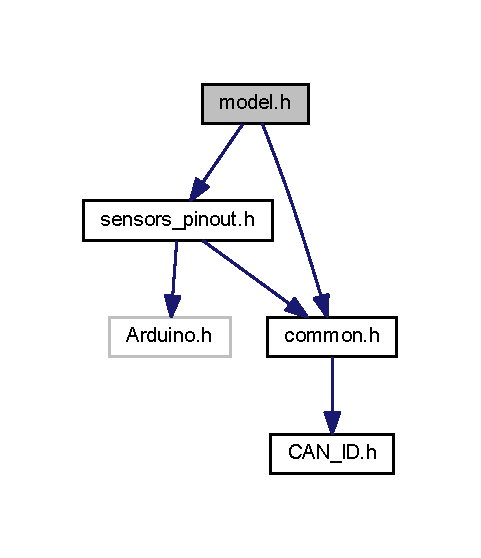
\includegraphics[width=231pt]{model_8h__incl}
\end{center}
\end{figure}
This graph shows which files directly or indirectly include this file\+:\nopagebreak
\begin{figure}[H]
\begin{center}
\leavevmode
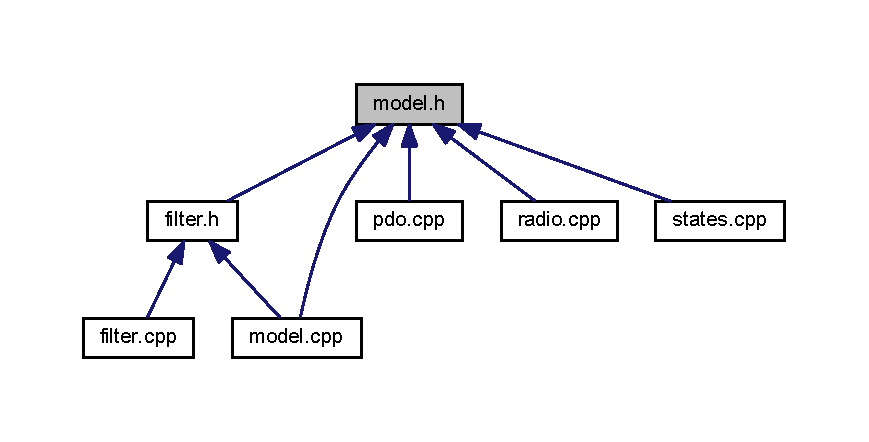
\includegraphics[width=350pt]{model_8h__dep__incl}
\end{center}
\end{figure}
\subsection*{Macros}
\begin{DoxyCompactItemize}
\item 
\#define \mbox{\hyperlink{group___board__model__group_gafd34b4e5a1067ffe9bfb1cb18b5973e6}{S\+U\+S\+P\+\_\+\+S\+T\+R\+O\+K\+E\+\_\+\+E\+X\+T\+E\+N\+S\+I\+ON}}~75.\+0
\begin{DoxyCompactList}\small\item\em Maximum suspension stroke \mbox{[} $mm$\mbox{]}. \end{DoxyCompactList}\end{DoxyCompactItemize}
\subsection*{Functions}
\begin{DoxyCompactItemize}
\item 
volatile uint16\+\_\+t \mbox{\hyperlink{group___board__model__group_ga77eb7343baa6cbfd81673dcbd03ac125}{get\+\_\+fr\+\_\+sx\+\_\+rpm}} ()
\begin{DoxyCompactList}\small\item\em If rpm value is lower than \mbox{\hyperlink{group___board__model__group_gafc05771487f188ffa40b6620afc1a9bc}{R\+P\+M\+\_\+\+M\+IN}}, output is forced to zero. \end{DoxyCompactList}\item 
volatile uint16\+\_\+t \mbox{\hyperlink{group___board__model__group_ga3f71b1feaa9b3356080597de5de12f7b}{get\+\_\+fr\+\_\+dx\+\_\+rpm}} ()
\begin{DoxyCompactList}\small\item\em If rpm value is lower than \mbox{\hyperlink{group___board__model__group_gafc05771487f188ffa40b6620afc1a9bc}{R\+P\+M\+\_\+\+M\+IN}}, output is forced to zero. \end{DoxyCompactList}\item 
volatile uint16\+\_\+t \mbox{\hyperlink{group___board__model__group_ga81c1dfd585ff1f0b26b38148909e064c}{get\+\_\+rt\+\_\+sx\+\_\+rpm}} ()
\begin{DoxyCompactList}\small\item\em This function returns retro left wheel velocity \mbox{[} $rpm$\mbox{]}. \end{DoxyCompactList}\item 
volatile uint16\+\_\+t \mbox{\hyperlink{group___board__model__group_ga812f59d2bf258b811a7ff9184ba23e78}{get\+\_\+rt\+\_\+dx\+\_\+rpm}} ()
\begin{DoxyCompactList}\small\item\em This function returns retro right wheel velocity \mbox{[} $rpm$\mbox{]}. \end{DoxyCompactList}\item 
void \mbox{\hyperlink{group___board__model__group_gace5a444da39d4366693503c53f0841c2}{model\+\_\+init}} ()
\begin{DoxyCompactList}\small\item\em This function initializes hardware board. \end{DoxyCompactList}\end{DoxyCompactItemize}
\subsection*{Variables}
\begin{DoxyCompactItemize}
\item 
volatile uint8\+\_\+t \mbox{\hyperlink{group___board__model__group_ga1d42f28ccf027a3243fad064fa47ef81}{tps1\+\_\+percentage}}
\begin{DoxyCompactList}\small\item\em First A\+P\+PS percentage value retrieved by tps1 signal (\mbox{\hyperlink{group___board__pinout__group_gae9aa914854f611488701c96a330b0bd4}{T\+P\+S1\+\_\+\+P\+IN}}) \end{DoxyCompactList}\item 
volatile uint8\+\_\+t \mbox{\hyperlink{group___board__model__group_gaf69d82f83885abc5adbd5fcbf4c421cf}{tps2\+\_\+percentage}}
\begin{DoxyCompactList}\small\item\em Second A\+P\+PS percentage value retrieved by tps2 signal (\mbox{\hyperlink{group___board__pinout__group_gab13a816bae3ca994897fc6f1cb590a67}{T\+P\+S2\+\_\+\+P\+IN}}) \end{DoxyCompactList}\item 
volatile uint8\+\_\+t \mbox{\hyperlink{group___board__model__group_ga8e50a30864da7026531520887968d4c0}{brake\+\_\+percentage}}
\begin{DoxyCompactList}\small\item\em Brake pedal position sensor percentage value retrieved by brake signal (\mbox{\hyperlink{group___board__pinout__group_gad632b56bf4c6259a390c3db91607078e}{B\+R\+A\+K\+E\+\_\+\+P\+IN}}) \end{DoxyCompactList}\item 
volatile bool \mbox{\hyperlink{group___board__model__group_gaa9de48f5a49bc92a608ed315c087f3a6}{apps\+\_\+plausibility}}
\begin{DoxyCompactList}\small\item\em A\+P\+PS plausibility status. \end{DoxyCompactList}\item 
volatile bool \mbox{\hyperlink{group___board__model__group_gae505d69d6ac9d4e7e3c2268ca6cb20b3}{brake\+\_\+plausibility}}
\begin{DoxyCompactList}\small\item\em Brake plausibility status. \end{DoxyCompactList}\item 
volatile uint8\+\_\+t \mbox{\hyperlink{group___board__model__group_ga90c23c0b7f858714327ef390c73f6424}{fr\+\_\+sx\+\_\+susp}}
\begin{DoxyCompactList}\small\item\em Frontal left suspension stroke \mbox{[} $mm$\mbox{]}. \end{DoxyCompactList}\item 
volatile uint8\+\_\+t \mbox{\hyperlink{group___board__model__group_ga4c01ad4d4fed642cd36faa3afcc78ffc}{fr\+\_\+dx\+\_\+susp}}
\begin{DoxyCompactList}\small\item\em Frontal right suspension stroke \mbox{[} $mm$\mbox{]}. \end{DoxyCompactList}\item 
volatile uint16\+\_\+t \mbox{\hyperlink{group___board__model__group_ga60aba8dcb458993e90d55d74c2b78f61}{fr\+\_\+sx\+\_\+rpm}}
\begin{DoxyCompactList}\small\item\em Frontal left wheel velocity \mbox{[} $rpm$\mbox{]}. \end{DoxyCompactList}\item 
volatile uint16\+\_\+t \mbox{\hyperlink{group___board__model__group_ga7ef4b53bcdb3160d25627fcf012408ea}{fr\+\_\+dx\+\_\+rpm}}
\begin{DoxyCompactList}\small\item\em Frontal right wheel velocity \mbox{[} $rpm$\mbox{]}. \end{DoxyCompactList}\item 
volatile uint8\+\_\+t \mbox{\hyperlink{group___board__model__group_ga9a397cb2df09e12e11a80e4f3fee8a1e}{acc\+\_\+x\+\_\+value}}
\begin{DoxyCompactList}\small\item\em Accelerometer X value \mbox{[} $m/s^{2}$\mbox{]}. \end{DoxyCompactList}\item 
volatile uint8\+\_\+t \mbox{\hyperlink{group___board__model__group_ga4779043af8ceac73610675efc457aaaf}{acc\+\_\+z\+\_\+value}}
\begin{DoxyCompactList}\small\item\em Accelerometer Z value \mbox{[} $m/s^{2}$\mbox{]}. \end{DoxyCompactList}\item 
volatile uint8\+\_\+t \mbox{\hyperlink{group___board__model__group_gaf3ea4d8836939176bd6b4f994518e4c8}{rt\+\_\+sx\+\_\+susp}}
\begin{DoxyCompactList}\small\item\em Retro left suspension stroke \mbox{[} $mm$\mbox{]}. \end{DoxyCompactList}\item 
volatile uint8\+\_\+t \mbox{\hyperlink{group___board__model__group_ga6b55629e8341a3f0e9143ec931712dba}{rt\+\_\+dx\+\_\+susp}}
\begin{DoxyCompactList}\small\item\em Retro right suspension stroke \mbox{[} $mm$\mbox{]}. \end{DoxyCompactList}\end{DoxyCompactItemize}


\subsection{Detailed Description}
Board model header file. 

\begin{DoxyAuthor}{Author}
Arella Matteo ~\newline
 (mail\+: \href{mailto:arella.1646983@studenti.uniroma1.it}{\tt arella.\+1646983@studenti.\+uniroma1.\+it}) 
\end{DoxyAuthor}
\begin{DoxyDate}{Date}
2018 
\end{DoxyDate}

\hypertarget{nmt_8cpp}{}\section{nmt.\+cpp File Reference}
\label{nmt_8cpp}\index{nmt.\+cpp@{nmt.\+cpp}}


C\+A\+N\+Open N\+MT module implementation file.  


{\ttfamily \#include \char`\"{}def.\+h\char`\"{}}\newline
{\ttfamily \#include \char`\"{}nmt.\+h\char`\"{}}\newline
{\ttfamily \#include \char`\"{}states.\+h\char`\"{}}\newline
Include dependency graph for nmt.\+cpp\+:\nopagebreak
\begin{figure}[H]
\begin{center}
\leavevmode
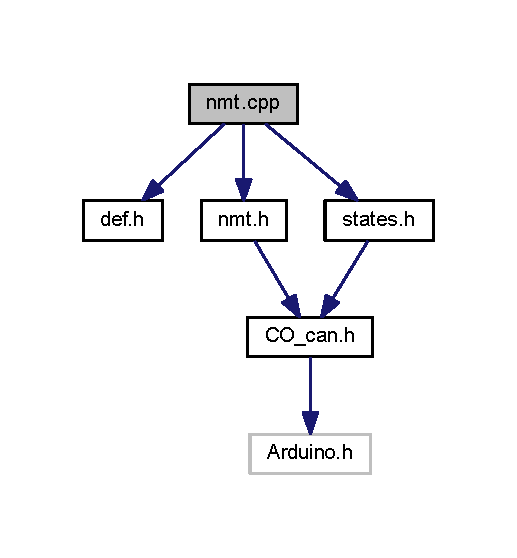
\includegraphics[width=248pt]{nmt_8cpp__incl}
\end{center}
\end{figure}
\subsection*{Functions}
\begin{DoxyCompactItemize}
\item 
void \mbox{\hyperlink{group___c_a_nopen___n_m_t__group_ga4f3ea874d17be7eefe09f3d8fcd9fc76}{proceed\+N\+M\+Tstate\+Change}} (\mbox{\hyperlink{struct_message}{Message}} $\ast$m)
\begin{DoxyCompactList}\small\item\em According to \mbox{\hyperlink{group___c_a_nopen___n_m_t__speficications}{C\+A\+Nopen N\+MT Command Specifiers}}, upon N\+MT reception from V\+CU master node, S\+CU change current state. \end{DoxyCompactList}\item 
void \mbox{\hyperlink{group___c_a_nopen___n_m_t__group_ga26588b389853484f581977032c0e1021}{slave\+Send\+Boot\+Up}} ()
\begin{DoxyCompactList}\small\item\em This function sends a slave boot-\/up message over C\+AN servizi network. \end{DoxyCompactList}\end{DoxyCompactItemize}


\subsection{Detailed Description}
C\+A\+N\+Open N\+MT module implementation file. 

\begin{DoxyAuthor}{Author}
Arella Matteo ~\newline
 (mail\+: \href{mailto:arella.1646983@studenti.uniroma1.it}{\tt arella.\+1646983@studenti.\+uniroma1.\+it}) 
\end{DoxyAuthor}
\begin{DoxyDate}{Date}
2018 
\end{DoxyDate}

\hypertarget{nmt_8h}{}\section{nmt.\+h File Reference}
\label{nmt_8h}\index{nmt.\+h@{nmt.\+h}}


C\+A\+N\+Open N\+MT module header.  


{\ttfamily \#include \char`\"{}C\+O\+\_\+can.\+h\char`\"{}}\newline
Include dependency graph for nmt.\+h\+:\nopagebreak
\begin{figure}[H]
\begin{center}
\leavevmode
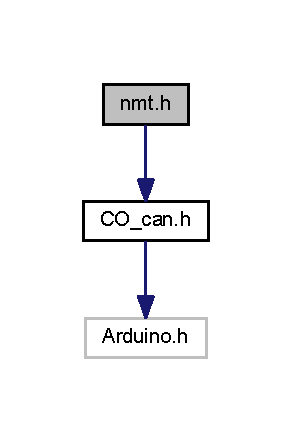
\includegraphics[width=217pt]{nmt_8h__incl}
\end{center}
\end{figure}
This graph shows which files directly or indirectly include this file\+:\nopagebreak
\begin{figure}[H]
\begin{center}
\leavevmode
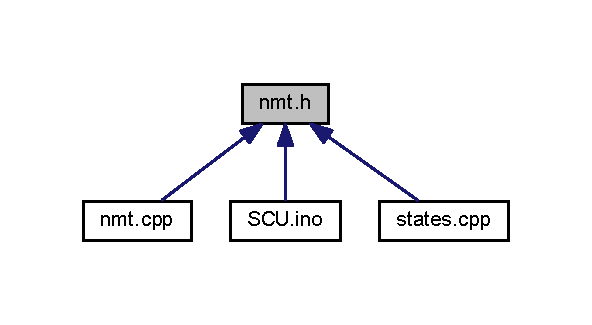
\includegraphics[width=284pt]{nmt_8h__dep__incl}
\end{center}
\end{figure}
\subsection*{Functions}
\begin{DoxyCompactItemize}
\item 
void \mbox{\hyperlink{group___c_a_nopen___n_m_t__group_ga4f3ea874d17be7eefe09f3d8fcd9fc76}{proceed\+N\+M\+Tstate\+Change}} (\mbox{\hyperlink{struct_message}{Message}} $\ast$m)
\begin{DoxyCompactList}\small\item\em According to \mbox{\hyperlink{group___c_a_nopen___n_m_t__speficications}{C\+A\+Nopen N\+MT Command Specifiers}}, upon N\+MT reception from V\+CU master node, S\+CU change current state. \end{DoxyCompactList}\item 
void \mbox{\hyperlink{group___c_a_nopen___n_m_t__group_ga26588b389853484f581977032c0e1021}{slave\+Send\+Boot\+Up}} ()
\begin{DoxyCompactList}\small\item\em This function sends a slave boot-\/up message over C\+AN servizi network. \end{DoxyCompactList}\end{DoxyCompactItemize}


\subsection{Detailed Description}
C\+A\+N\+Open N\+MT module header. 

\begin{DoxyAuthor}{Author}
Arella Matteo ~\newline
 (mail\+: \href{mailto:arella.1646983@studenti.uniroma1.it}{\tt arella.\+1646983@studenti.\+uniroma1.\+it}) 
\end{DoxyAuthor}
\begin{DoxyDate}{Date}
2018 
\end{DoxyDate}

\hypertarget{pdo_8cpp}{}\section{pdo.\+cpp File Reference}
\label{pdo_8cpp}\index{pdo.\+cpp@{pdo.\+cpp}}


C\+A\+Nopen P\+DO support header file.  


{\ttfamily \#include \char`\"{}pdo.\+h\char`\"{}}\newline
{\ttfamily \#include \char`\"{}states.\+h\char`\"{}}\newline
{\ttfamily \#include \char`\"{}model.\+h\char`\"{}}\newline
Include dependency graph for pdo.\+cpp\+:\nopagebreak
\begin{figure}[H]
\begin{center}
\leavevmode
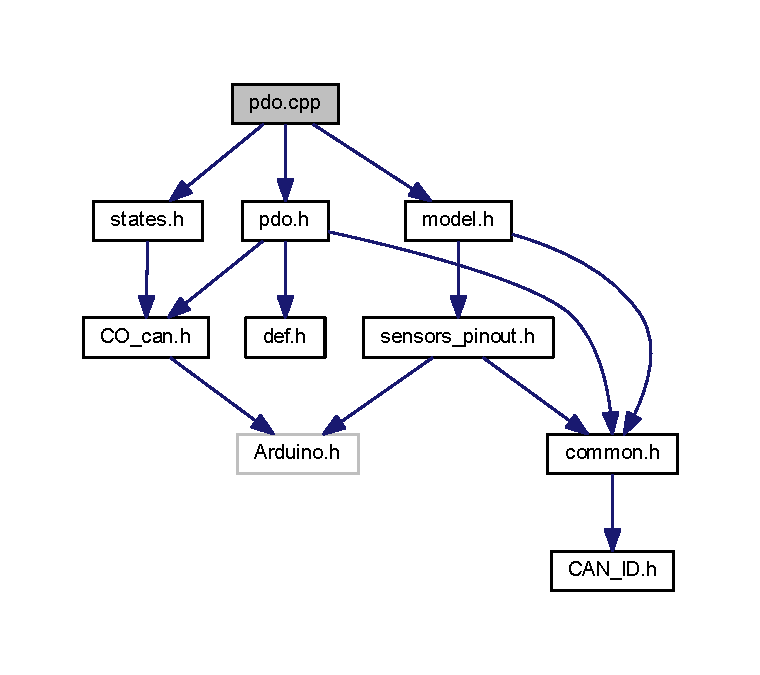
\includegraphics[width=350pt]{pdo_8cpp__incl}
\end{center}
\end{figure}
\subsection*{Functions}
\begin{DoxyCompactItemize}
\item 
void \mbox{\hyperlink{group___c_a_nopen___p_d_o__module_gac0ec660dbbba1d5ab27615147f369caf}{build\+P\+DO}} (uint8\+\_\+t P\+D\+Otype, \mbox{\hyperlink{struct_message}{Message}} $\ast$pdo)
\begin{DoxyCompactList}\small\item\em This function serializes data to send into P\+DO message. \end{DoxyCompactList}\item 
void \mbox{\hyperlink{group___c_a_nopen___p_d_o__module_ga91f92516824d9dc33dc8cf83b34726e1}{proceed\+P\+DO}} (\mbox{\hyperlink{struct_message}{Message}} $\ast$pdo)
\begin{DoxyCompactList}\small\item\em This function manages P\+DO message receive, deserializing data. \end{DoxyCompactList}\end{DoxyCompactItemize}


\subsection{Detailed Description}
C\+A\+Nopen P\+DO support header file. 

\begin{DoxyAuthor}{Author}
Arella Matteo ~\newline
 (mail\+: \href{mailto:arella.1646983@studenti.uniroma1.it}{\tt arella.\+1646983@studenti.\+uniroma1.\+it}) 
\end{DoxyAuthor}
\begin{DoxyDate}{Date}
2018 
\end{DoxyDate}

\hypertarget{pdo_8h}{}\section{pdo.\+h File Reference}
\label{pdo_8h}\index{pdo.\+h@{pdo.\+h}}


C\+A\+Nopen P\+DO support header file.  


{\ttfamily \#include \char`\"{}def.\+h\char`\"{}}\newline
{\ttfamily \#include \char`\"{}C\+O\+\_\+can.\+h\char`\"{}}\newline
{\ttfamily \#include \char`\"{}common.\+h\char`\"{}}\newline
Include dependency graph for pdo.\+h\+:\nopagebreak
\begin{figure}[H]
\begin{center}
\leavevmode
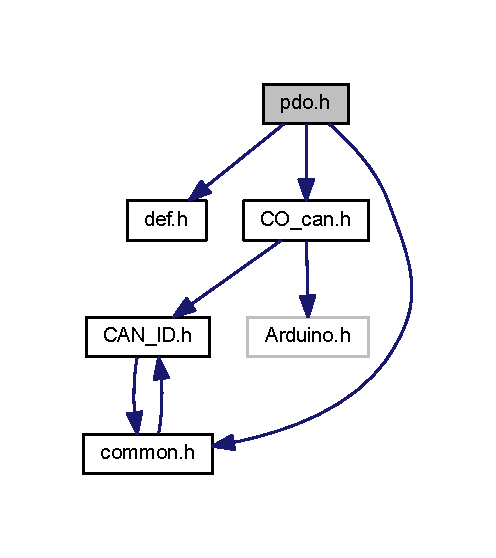
\includegraphics[width=276pt]{pdo_8h__incl}
\end{center}
\end{figure}
This graph shows which files directly or indirectly include this file\+:\nopagebreak
\begin{figure}[H]
\begin{center}
\leavevmode
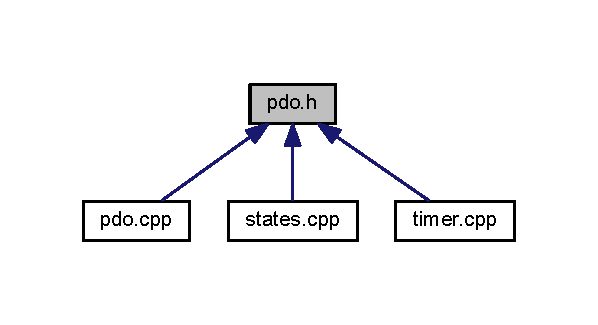
\includegraphics[width=287pt]{pdo_8h__dep__incl}
\end{center}
\end{figure}
\subsection*{Functions}
\begin{DoxyCompactItemize}
\item 
void \mbox{\hyperlink{group___c_a_nopen___p_d_o__module_gac0ec660dbbba1d5ab27615147f369caf}{build\+P\+DO}} (uint8\+\_\+t P\+D\+Otype, \mbox{\hyperlink{struct_message}{Message}} $\ast$pdo)
\begin{DoxyCompactList}\small\item\em This function serializes data to send into P\+DO message. \end{DoxyCompactList}\item 
void \mbox{\hyperlink{group___c_a_nopen___p_d_o__module_ga91f92516824d9dc33dc8cf83b34726e1}{proceed\+P\+DO}} (\mbox{\hyperlink{struct_message}{Message}} $\ast$pdo)
\begin{DoxyCompactList}\small\item\em This function manages P\+DO message receive, deserializing data. \end{DoxyCompactList}\end{DoxyCompactItemize}


\subsection{Detailed Description}
C\+A\+Nopen P\+DO support header file. 

\begin{DoxyAuthor}{Author}
Arella Matteo ~\newline
 (mail\+: \href{mailto:arella.1646983@studenti.uniroma1.it}{\tt arella.\+1646983@studenti.\+uniroma1.\+it}) 
\end{DoxyAuthor}
\begin{DoxyDate}{Date}
2018 
\end{DoxyDate}

\hypertarget{radio_8cpp}{}\section{radio.\+cpp File Reference}
\label{radio_8cpp}\index{radio.\+cpp@{radio.\+cpp}}


Radio implementation file.  


{\ttfamily \#include \char`\"{}radio.\+h\char`\"{}}\newline
{\ttfamily \#include $<$S\+P\+I.\+h$>$}\newline
{\ttfamily \#include $<$n\+R\+F24\+L01.\+h$>$}\newline
{\ttfamily \#include $<$R\+F24.\+h$>$}\newline
{\ttfamily \#include $<$Arduino.\+h$>$}\newline
{\ttfamily \#include $<$Arduino\+Json.\+h$>$}\newline
{\ttfamily \#include $<$Base64.\+h$>$}\newline
{\ttfamily \#include \char`\"{}sensors\+\_\+pinout.\+h\char`\"{}}\newline
{\ttfamily \#include \char`\"{}model.\+h\char`\"{}}\newline
{\ttfamily \#include \char`\"{}aes.\+h\char`\"{}}\newline
Include dependency graph for radio.\+cpp\+:\nopagebreak
\begin{figure}[H]
\begin{center}
\leavevmode
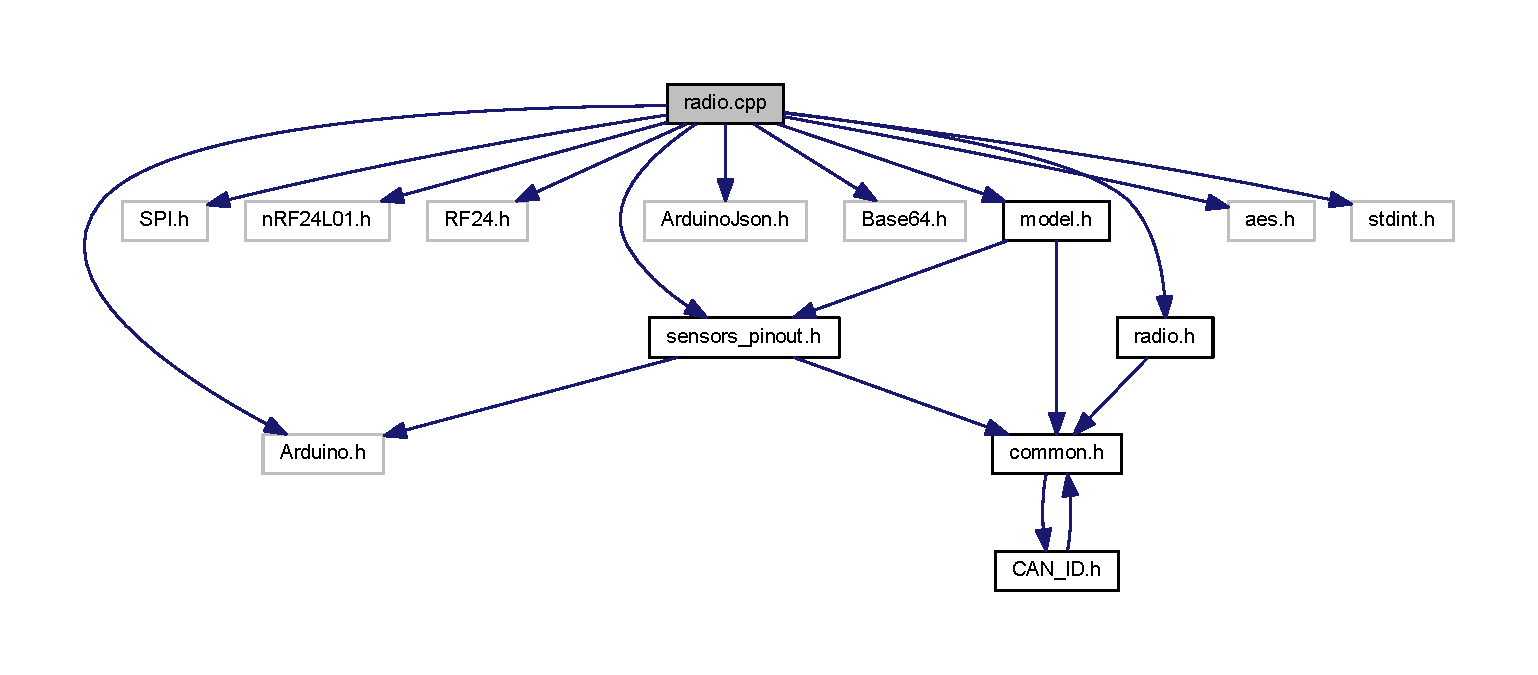
\includegraphics[width=350pt]{radio_8cpp__incl}
\end{center}
\end{figure}
\subsection*{Macros}
\begin{DoxyCompactItemize}
\item 
\#define \mbox{\hyperlink{group___radio__module_gaa445a79fc0f7373036c72d198e51f19a}{C\+TR}}~1
\begin{DoxyCompactList}\small\item\em Enable/\+Disable aes C\+TR mode. \end{DoxyCompactList}\item 
\#define \mbox{\hyperlink{group___radio__module_gaf0e9fea2a1fefbbf655ad908e653fa37}{R\+A\+D\+I\+O\+\_\+\+K\+E\+Y\+\_\+\+B\+I\+TS}}~192
\begin{DoxyCompactList}\small\item\em Aes key length \mbox{[} $bits$\mbox{]}. \end{DoxyCompactList}\item 
\#define \mbox{\hyperlink{group___radio__module_ga2e4ba70a12e464d5b5278c18d28355f8}{J\+S\+O\+N\+\_\+\+B\+U\+F\+F\+E\+R\+\_\+\+S\+I\+ZE}}~J\+S\+O\+N\+\_\+\+O\+B\+J\+E\+C\+T\+\_\+\+S\+I\+ZE(2) + 3 $\ast$ J\+S\+O\+N\+\_\+\+O\+B\+J\+E\+C\+T\+\_\+\+S\+I\+ZE(4) + J\+S\+O\+N\+\_\+\+O\+B\+J\+E\+C\+T\+\_\+\+S\+I\+ZE(5) + 219
\begin{DoxyCompactList}\small\item\em Size of static buffer for J\+S\+ON serialization, generated by \href{https://arduinojson.org/assistant/}{\tt https\+://arduinojson.\+org/assistant/}. Model serialization format\+: \end{DoxyCompactList}\item 
\#define \mbox{\hyperlink{group___radio__module_gae634b89476ef10a9d21eacb0da28cd7b}{C\+I\+P\+H\+E\+R\+\_\+\+M\+A\+X\+\_\+\+L\+E\+N\+G\+TH}}~1024
\begin{DoxyCompactList}\small\item\em Cipher buffer max length (according to \href{https://arduinojson.org/assistant/}{\tt https\+://arduinojson.\+org/assistant/}). \end{DoxyCompactList}\item 
\#define \mbox{\hyperlink{group___radio__module_ga35dc4d7d23c1b86227ceb68e6ebc4fc2}{I\+V\+\_\+\+L\+EN}}~A\+E\+S\+\_\+\+K\+E\+Y\+L\+EN
\begin{DoxyCompactList}\small\item\em Initialization Vector length. \end{DoxyCompactList}\end{DoxyCompactItemize}
\subsection*{Functions}
\begin{DoxyCompactItemize}
\item 
R\+F24 \mbox{\hyperlink{group___radio__module_gab473f61dd66af21e8f24b4b95dca0222}{radio}} (R\+A\+D\+I\+O\+\_\+\+C\+E\+\_\+\+P\+IN, R\+A\+D\+I\+O\+\_\+\+C\+S\+N\+\_\+\+P\+IN)
\begin{DoxyCompactList}\small\item\em Radio. \end{DoxyCompactList}\item 
void \mbox{\hyperlink{group___radio__module_ga42ee2daa57d1e88e4ca6c712dba5039a}{encrypt\+\_\+model}} (char $\ast$buffer, char $\ast$\mbox{\hyperlink{group___radio__module_ga352378cd7d5875f33dece696475cb8d4}{iv}}, uint16\+\_\+t plain\+\_\+len, uint16\+\_\+t buffer\+\_\+len)
\begin{DoxyCompactList}\small\item\em Encrypt model for transmit over radio. \end{DoxyCompactList}\item 
volatile char \mbox{\hyperlink{group___radio__module_ga7eb1db79bc6e9408f447ffdc65c09aaa}{generate\+\_\+random\+\_\+char}} ()
\begin{DoxyCompactList}\small\item\em Generate a Cryptgraphically secure pseudorandom number from T\+R\+NG hardware peripheral. \end{DoxyCompactList}\item 
void \mbox{\hyperlink{group___radio__module_ga8d208a46c01313ddc1320256e3ce607d}{generate\+\_\+iv}} (char $\ast$buffer, uint16\+\_\+t len)
\begin{DoxyCompactList}\small\item\em Generate a randomized initialization vector. \end{DoxyCompactList}\item 
void \mbox{\hyperlink{group___radio__module_gad2c532e768a8351b48ffcc95dc56e912}{pkcs7\+\_\+padding}} (char $\ast$buffer, uint16\+\_\+t plain\+\_\+len, uint16\+\_\+t buffer\+\_\+len)
\begin{DoxyCompactList}\small\item\em Perform P\+K\+C\+S7 padding described in R\+FC 5652. \end{DoxyCompactList}\item 
void \mbox{\hyperlink{group___radio__module_ga2cca2e5e5a5f34888f1801e752c29eb3}{byte\+\_\+padding}} (char $\ast$buffer, uint16\+\_\+t plain\+\_\+len, uint16\+\_\+t buffer\+\_\+len)
\begin{DoxyCompactList}\small\item\em Perform I\+S\+O/\+I\+EC 7816-\/4 byte padding. \end{DoxyCompactList}\item 
void \mbox{\hyperlink{group___radio__module_gaaf9aff6a522103cc312457043baf7eca}{radio\+\_\+init}} ()
\begin{DoxyCompactList}\small\item\em Initialize T\+R\+NG (True Random Number Generator) hardware peripheral as a C\+S\+P\+R\+NG (Cryptographically Secure Pseudo-\/\+Random Number Generator) for generate randomized IV. \end{DoxyCompactList}\item 
void \mbox{\hyperlink{group___radio__module_ga5250a82de95a2d4e497dd1c580a92362}{radio\+\_\+send\+\_\+model}} ()
\begin{DoxyCompactList}\small\item\em Actions performed involve\+: \end{DoxyCompactList}\end{DoxyCompactItemize}
\subsection*{Variables}
\begin{DoxyCompactItemize}
\item 
volatile bool \mbox{\hyperlink{group___radio__module_gaaebbe13533cac0f28446c13ae32b1cb2}{radio\+\_\+transmit}} = false
\begin{DoxyCompactList}\small\item\em Radio transmit enable flag. \end{DoxyCompactList}\item 
char \mbox{\hyperlink{group___radio__module_gae0c804caa6b80b155884dc4f7a2d9da3}{key}} \mbox{[}A\+E\+S\+\_\+\+K\+E\+Y\+L\+EN\mbox{]}
\begin{DoxyCompactList}\small\item\em A\+ES encryption K\+EY. \end{DoxyCompactList}\item 
char \mbox{\hyperlink{group___radio__module_ga352378cd7d5875f33dece696475cb8d4}{iv}} \mbox{[}\mbox{\hyperlink{group___radio__module_ga35dc4d7d23c1b86227ceb68e6ebc4fc2}{I\+V\+\_\+\+L\+EN}}+1\mbox{]}
\begin{DoxyCompactList}\small\item\em A\+ES encryption Initialization Vector. \end{DoxyCompactList}\item 
char \mbox{\hyperlink{group___radio__module_ga4372a894c9299a437425452130748eb8}{cipher}} \mbox{[}\mbox{\hyperlink{group___radio__module_gae634b89476ef10a9d21eacb0da28cd7b}{C\+I\+P\+H\+E\+R\+\_\+\+M\+A\+X\+\_\+\+L\+E\+N\+G\+TH}}+1\mbox{]} = \{0\}
\begin{DoxyCompactList}\small\item\em Encrypted model buffer. \end{DoxyCompactList}\item 
const uint64\+\_\+t \mbox{\hyperlink{group___radio__module_gafe30685f23b8cbf122ddec37280ba8e4}{pipe}} = 0x\+E8\+E8\+F0\+F0\+E1\+LL
\begin{DoxyCompactList}\small\item\em Radio writing pipe. \end{DoxyCompactList}\end{DoxyCompactItemize}


\subsection{Detailed Description}
Radio implementation file. 

\begin{DoxyAuthor}{Author}
Arella Matteo ~\newline
 (mail\+: \href{mailto:arella.1646983@studenti.uniroma1.it}{\tt arella.\+1646983@studenti.\+uniroma1.\+it}) 
\end{DoxyAuthor}
\begin{DoxyDate}{Date}
2018 
\end{DoxyDate}

\hypertarget{radio_8h}{}\section{radio.\+h File Reference}
\label{radio_8h}\index{radio.\+h@{radio.\+h}}


Radio header file.  


{\ttfamily \#include \char`\"{}common.\+h\char`\"{}}\newline
Include dependency graph for radio.\+h\+:\nopagebreak
\begin{figure}[H]
\begin{center}
\leavevmode
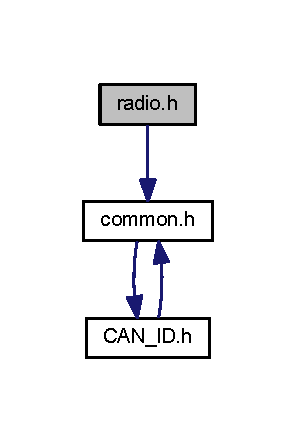
\includegraphics[width=142pt]{radio_8h__incl}
\end{center}
\end{figure}
This graph shows which files directly or indirectly include this file\+:\nopagebreak
\begin{figure}[H]
\begin{center}
\leavevmode
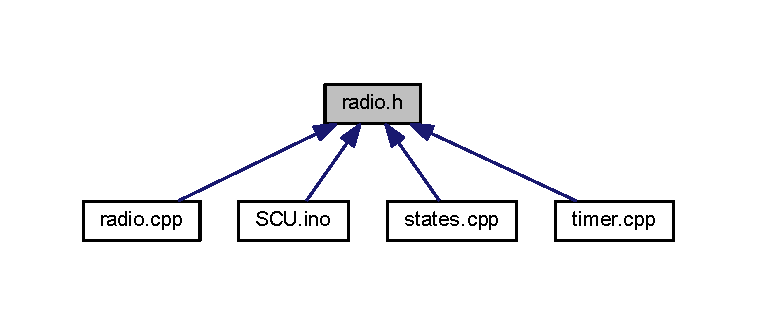
\includegraphics[width=350pt]{radio_8h__dep__incl}
\end{center}
\end{figure}
\subsection*{Functions}
\begin{DoxyCompactItemize}
\item 
void \mbox{\hyperlink{group___radio__module_gaaf9aff6a522103cc312457043baf7eca}{radio\+\_\+init}} ()
\begin{DoxyCompactList}\small\item\em Initialize T\+R\+NG (True Random Number Generator) hardware peripheral as a C\+S\+P\+R\+NG (Cryptographically Secure Pseudo-\/\+Random Number Generator) for generate randomized IV. \end{DoxyCompactList}\item 
void \mbox{\hyperlink{group___radio__module_ga5250a82de95a2d4e497dd1c580a92362}{radio\+\_\+send\+\_\+model}} ()
\begin{DoxyCompactList}\small\item\em Actions performed involve\+: \end{DoxyCompactList}\end{DoxyCompactItemize}
\subsection*{Variables}
\begin{DoxyCompactItemize}
\item 
volatile bool \mbox{\hyperlink{group___radio__module_gaaebbe13533cac0f28446c13ae32b1cb2}{radio\+\_\+transmit}}
\begin{DoxyCompactList}\small\item\em Radio transmit enable flag. \end{DoxyCompactList}\end{DoxyCompactItemize}


\subsection{Detailed Description}
Radio header file. 

\begin{DoxyAuthor}{Author}
Arella Matteo ~\newline
 (mail\+: \href{mailto:arella.1646983@studenti.uniroma1.it}{\tt arella.\+1646983@studenti.\+uniroma1.\+it}) 
\end{DoxyAuthor}
\begin{DoxyDate}{Date}
2018 
\end{DoxyDate}

\hypertarget{_s_c_u_8ino}{}\section{S\+C\+U.\+ino File Reference}
\label{_s_c_u_8ino}\index{S\+C\+U.\+ino@{S\+C\+U.\+ino}}


Main module file.  


{\ttfamily \#include \char`\"{}common.\+h\char`\"{}}\newline
{\ttfamily \#include \char`\"{}states.\+h\char`\"{}}\newline
{\ttfamily \#include \char`\"{}nmt.\+h\char`\"{}}\newline
{\ttfamily \#include \char`\"{}radio.\+h\char`\"{}}\newline
Include dependency graph for S\+C\+U.\+ino\+:\nopagebreak
\begin{figure}[H]
\begin{center}
\leavevmode
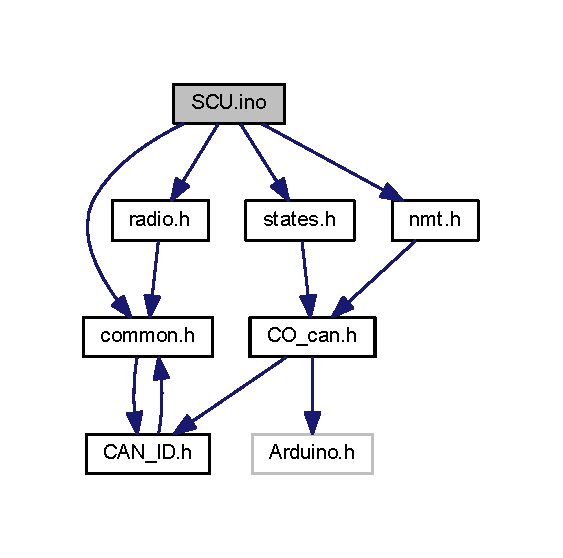
\includegraphics[width=311pt]{_s_c_u_8ino__incl}
\end{center}
\end{figure}
\subsection*{Functions}
\begin{DoxyCompactItemize}
\item 
void \mbox{\hyperlink{group___main__group__module_ga4fc01d736fe50cf5b977f755b675f11d}{setup}} ()
\begin{DoxyCompactList}\small\item\em This function perform basic board setup. Upon power-\/up S\+CU (C\+A\+Nopen slave node) goes into initialization. It initializes the entire application, C\+A\+N/\+C\+A\+Nopen interfaces and communication. At the end of the initialization the node tries to transmit boot-\/up message. As soon as it is transmitted successfully, the node switches to Pre-\/operational state. \end{DoxyCompactList}\item 
void \mbox{\hyperlink{group___main__group__module_gafe461d27b9c48d5921c00d521181f12f}{loop}} ()
\begin{DoxyCompactList}\small\item\em This function is called into endless while main loop. It takes care of sending data through radio, if enabled. \end{DoxyCompactList}\end{DoxyCompactItemize}


\subsection{Detailed Description}
Main module file. 

\begin{DoxyAuthor}{Author}
Arella Matteo ~\newline
 (mail\+: \href{mailto:arella.1646983@studenti.uniroma1.it}{\tt arella.\+1646983@studenti.\+uniroma1.\+it}) 
\end{DoxyAuthor}
\begin{DoxyDate}{Date}
2018 
\end{DoxyDate}

\hypertarget{sensors__pinout_8h}{}\section{sensors\+\_\+pinout.\+h File Reference}
\label{sensors__pinout_8h}\index{sensors\+\_\+pinout.\+h@{sensors\+\_\+pinout.\+h}}


Board pinout module header.  


{\ttfamily \#include $<$Arduino.\+h$>$}\newline
{\ttfamily \#include \char`\"{}common.\+h\char`\"{}}\newline
Include dependency graph for sensors\+\_\+pinout.\+h\+:\nopagebreak
\begin{figure}[H]
\begin{center}
\leavevmode
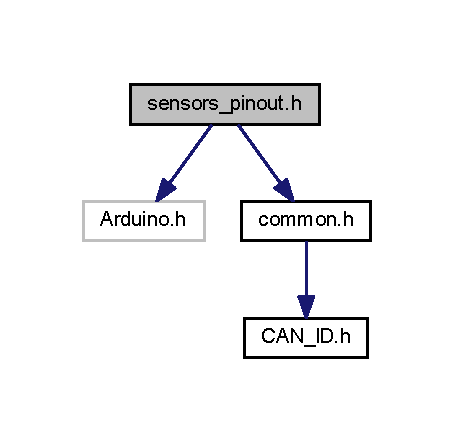
\includegraphics[width=218pt]{sensors__pinout_8h__incl}
\end{center}
\end{figure}
This graph shows which files directly or indirectly include this file\+:\nopagebreak
\begin{figure}[H]
\begin{center}
\leavevmode
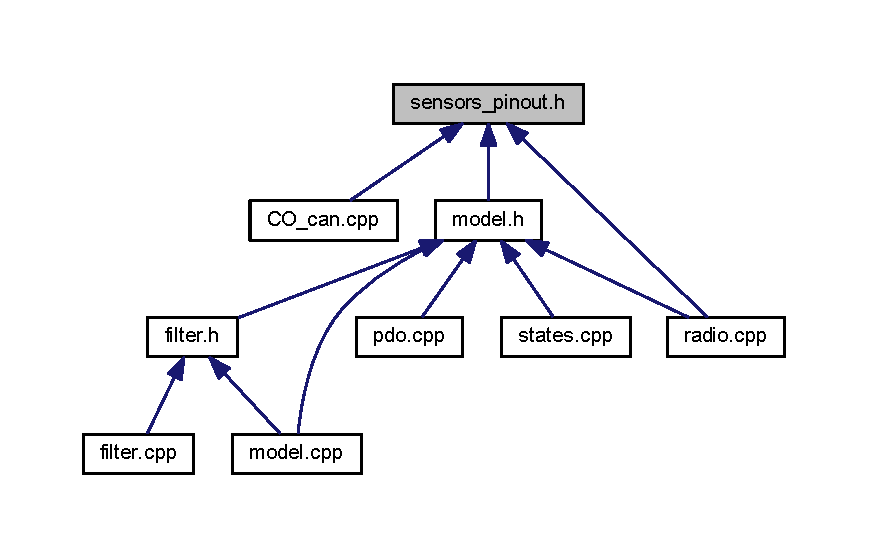
\includegraphics[width=350pt]{sensors__pinout_8h__dep__incl}
\end{center}
\end{figure}
\subsection*{Macros}
\begin{DoxyCompactItemize}
\item 
\#define \mbox{\hyperlink{group___board__pinout__group_gadaeb42d6b221ac2d3e0bd14f05aeefa5}{C\+A\+N\+\_\+\+P\+O\+RT}}~Can0
\begin{DoxyCompactList}\small\item\em Pin on board dedicated to C\+AN port. \end{DoxyCompactList}\item 
\#define \mbox{\hyperlink{group___board__pinout__group_gae9aa914854f611488701c96a330b0bd4}{T\+P\+S1\+\_\+\+P\+IN}}~A0
\begin{DoxyCompactList}\small\item\em Pin on board dedicated to first A\+P\+PS (tps1) \end{DoxyCompactList}\item 
\#define \mbox{\hyperlink{group___board__pinout__group_ga99b2a7dadaf495e3c559a46440f9141f}{T\+P\+S1\+\_\+\+A\+D\+C\+\_\+\+C\+H\+A\+N\+\_\+\+N\+UM}}~A\+D\+C\+\_\+\+C\+H\+E\+R\+\_\+\+C\+H7
\begin{DoxyCompactList}\small\item\em G\+P\+IO pin on the Atmel S\+A\+M3\+X8E processor corresponding to tps1 signal (A\+D7) \end{DoxyCompactList}\item 
\#define \mbox{\hyperlink{group___board__pinout__group_gab13a816bae3ca994897fc6f1cb590a67}{T\+P\+S2\+\_\+\+P\+IN}}~A1
\begin{DoxyCompactList}\small\item\em Pin on board dedicated to second A\+P\+PS (tps2) \end{DoxyCompactList}\item 
\#define \mbox{\hyperlink{group___board__pinout__group_ga4cecb8c10512873904099a1a88d69ed3}{T\+P\+S2\+\_\+\+A\+D\+C\+\_\+\+C\+H\+A\+N\+\_\+\+N\+UM}}~A\+D\+C\+\_\+\+C\+H\+E\+R\+\_\+\+C\+H6
\begin{DoxyCompactList}\small\item\em G\+P\+IO pin on the Atmel S\+A\+M3\+X8E processor corresponding to tps2 signal (A\+D6) \end{DoxyCompactList}\item 
\#define \mbox{\hyperlink{group___board__pinout__group_gad632b56bf4c6259a390c3db91607078e}{B\+R\+A\+K\+E\+\_\+\+P\+IN}}~A2
\begin{DoxyCompactList}\small\item\em Pin on board dedicated to brake pedal position sensor. \end{DoxyCompactList}\item 
\#define \mbox{\hyperlink{group___board__pinout__group_ga310547321c4a016c4ad19922920fadfd}{B\+R\+A\+K\+E\+\_\+\+A\+D\+C\+\_\+\+C\+H\+A\+N\+\_\+\+N\+UM}}~A\+D\+C\+\_\+\+C\+H\+E\+R\+\_\+\+C\+H5
\begin{DoxyCompactList}\small\item\em G\+P\+IO pin on the Atmel S\+A\+M3\+X8E processor corresponding to brake signal (A\+D5) \end{DoxyCompactList}\item 
\#define \mbox{\hyperlink{group___board__pinout__group_ga26973930bb94d493970560d50ed5388f}{F\+R\+\_\+\+S\+X\+\_\+\+S\+U\+S\+P\+\_\+\+P\+IN}}~A3
\begin{DoxyCompactList}\small\item\em Pin on board dedicated to frontal left suspension sensor. \end{DoxyCompactList}\item 
\#define \mbox{\hyperlink{group___board__pinout__group_gab536d8e8e876dfd8764cc1d31620803a}{F\+R\+\_\+\+S\+X\+\_\+\+A\+D\+C\+\_\+\+C\+H\+A\+N\+\_\+\+N\+UM}}~A\+D\+C\+\_\+\+C\+H\+E\+R\+\_\+\+C\+H4
\begin{DoxyCompactList}\small\item\em G\+P\+IO pin on the Atmel S\+A\+M3\+X8E processor corresponding to frontal left suspension signal (A\+D4) \end{DoxyCompactList}\item 
\#define \mbox{\hyperlink{group___board__pinout__group_gac6b52ca09115f1f82aa92ffd31363c05}{F\+R\+\_\+\+D\+X\+\_\+\+S\+U\+S\+P\+\_\+\+P\+IN}}~A4
\begin{DoxyCompactList}\small\item\em Pin on board dedicated to frontal right suspension sensor. \end{DoxyCompactList}\item 
\#define \mbox{\hyperlink{group___board__pinout__group_ga9d0085cf869db954c00e9c13d9661d51}{F\+R\+\_\+\+D\+X\+\_\+\+A\+D\+C\+\_\+\+C\+H\+A\+N\+\_\+\+N\+UM}}~A\+D\+C\+\_\+\+C\+H\+E\+R\+\_\+\+C\+H3
\begin{DoxyCompactList}\small\item\em G\+P\+IO pin on the Atmel S\+A\+M3\+X8E processor corresponding to frontal right suspension signal (A\+D3) \end{DoxyCompactList}\item 
\#define \mbox{\hyperlink{group___board__pinout__group_ga283872484ffa2d7043a08a80ff7a6cbc}{F\+R\+\_\+\+S\+X\+\_\+\+P\+W\+\_\+\+P\+IN}}~36
\begin{DoxyCompactList}\small\item\em Pin on board dedicated to frontal left phonic wheel encoder. \end{DoxyCompactList}\item 
\#define \mbox{\hyperlink{group___board__pinout__group_gad70d75cffb6389aff09c9d9b67a70777}{F\+R\+\_\+\+D\+X\+\_\+\+P\+W\+\_\+\+P\+IN}}~38
\begin{DoxyCompactList}\small\item\em Pin on board dedicated to frontal right phonic wheel encoder. \end{DoxyCompactList}\end{DoxyCompactItemize}


\subsection{Detailed Description}
Board pinout module header. 

\begin{DoxyAuthor}{Author}
Arella Matteo ~\newline
 (mail\+: \href{mailto:arella.1646983@studenti.uniroma1.it}{\tt arella.\+1646983@studenti.\+uniroma1.\+it}) 
\end{DoxyAuthor}
\begin{DoxyDate}{Date}
2018 
\end{DoxyDate}

\hypertarget{states_8cpp}{}\section{states.\+cpp File Reference}
\label{states_8cpp}\index{states.\+cpp@{states.\+cpp}}


C\+A\+Nopen finite state machine implementation file.  


{\ttfamily \#include \char`\"{}timer.\+h\char`\"{}}\newline
{\ttfamily \#include \char`\"{}def.\+h\char`\"{}}\newline
{\ttfamily \#include \char`\"{}pdo.\+h\char`\"{}}\newline
{\ttfamily \#include \char`\"{}states.\+h\char`\"{}}\newline
{\ttfamily \#include \char`\"{}nmt.\+h\char`\"{}}\newline
{\ttfamily \#include \char`\"{}C\+O\+\_\+can.\+h\char`\"{}}\newline
{\ttfamily \#include \char`\"{}common.\+h\char`\"{}}\newline
{\ttfamily \#include \char`\"{}model.\+h\char`\"{}}\newline
{\ttfamily \#include \char`\"{}radio.\+h\char`\"{}}\newline
Include dependency graph for states.\+cpp\+:\nopagebreak
\begin{figure}[H]
\begin{center}
\leavevmode
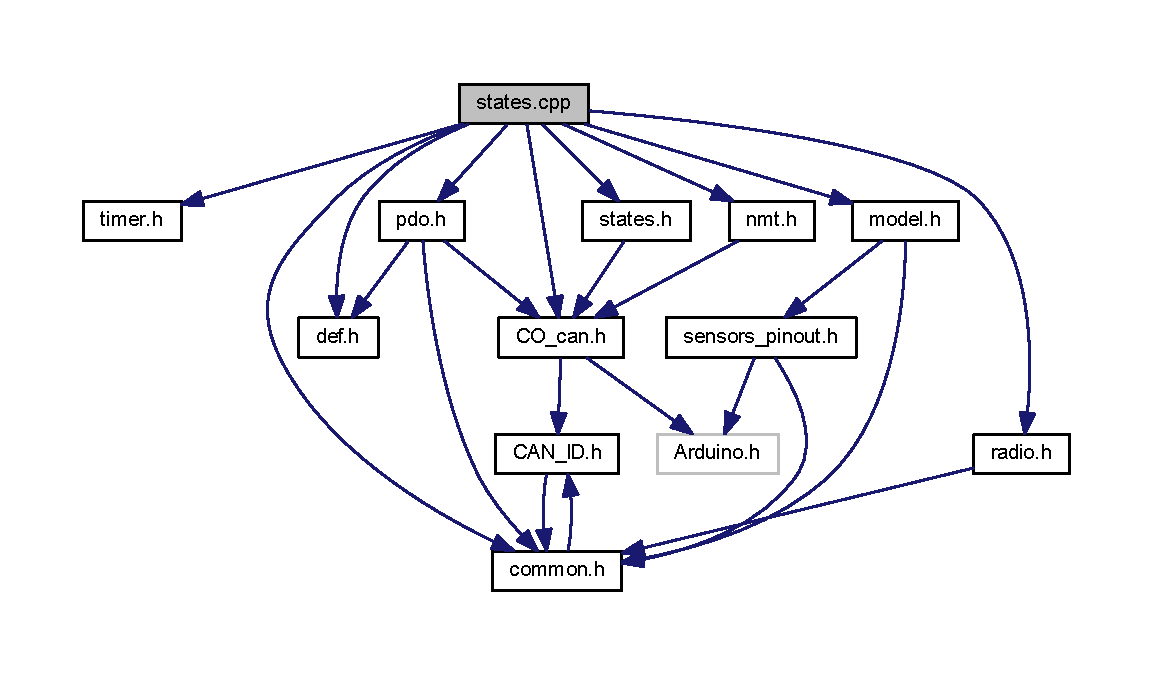
\includegraphics[width=350pt]{states_8cpp__incl}
\end{center}
\end{figure}
\subsection*{Functions}
\begin{DoxyCompactItemize}
\item 
\mbox{\hyperlink{group___c_a_nopen___f_s_m__module_ga5891f63a4c9243179838389a93d084e2}{e\+\_\+node\+State}} \mbox{\hyperlink{group___c_a_nopen___f_s_m__module_ga2802a8c3f0174f4e54dd2381968212a0}{get\+State}} ()
\begin{DoxyCompactList}\small\item\em Return current state on the \mbox{\hyperlink{_f_s_m_page}{Finite State Machine (F\+SM)}}. \end{DoxyCompactList}\item 
void \mbox{\hyperlink{group___c_a_nopen___f_s_m__module_ga47cb7615bbcf2c96cc4a7656f9a76bab}{set\+State}} (\mbox{\hyperlink{group___c_a_nopen___f_s_m__module_ga5891f63a4c9243179838389a93d084e2}{e\+\_\+node\+State}} new\+State)
\begin{DoxyCompactList}\small\item\em Set current state on the \mbox{\hyperlink{_f_s_m_page}{Finite State Machine (F\+SM)}}. \end{DoxyCompactList}\item 
void \mbox{\hyperlink{group___c_a_nopen___f_s_m__module_gabbbb23c086599a8d9432a2121ee82192}{can\+Dispatch}} (\mbox{\hyperlink{struct_message}{Message}} $\ast$m)
\begin{DoxyCompactList}\small\item\em Called by driver when receiving C\+A\+Nopen messages. \end{DoxyCompactList}\item 
void \mbox{\hyperlink{group___c_a_nopen___f_s_m__module_gadfffb3be7aa80aea898ada67e93d2388}{initialisation}} ()
\begin{DoxyCompactList}\small\item\em Initialize \mbox{\hyperlink{group___board__model__group}{Board module}}. If rear S\+CU firmware is selected (according to \mbox{\hyperlink{group___s_c_u__firmware__selection}{S\+CU firmware selection}}) radio is initialized. It initializes the entire application, C\+A\+N/\+C\+A\+Nopen interfaces and communication. \end{DoxyCompactList}\item 
void \mbox{\hyperlink{group___c_a_nopen___f_s_m__module_gaf9e8e3744244bcb2f8b6a8583c0bec0c}{pre\+Operational}} ()
\begin{DoxyCompactList}\small\item\em pre\+Operational state task on the F\+SM. \end{DoxyCompactList}\item 
void \mbox{\hyperlink{group___c_a_nopen___f_s_m__module_ga003b28d176774c489577f471a7b5f946}{operational}} ()
\begin{DoxyCompactList}\small\item\em Start timer for periodic T\+P\+DO transmit according to \mbox{\hyperlink{_c_a_n_network_page}{C\+AN Servizi network}}. \end{DoxyCompactList}\item 
void \mbox{\hyperlink{group___c_a_nopen___f_s_m__module_gad134c6ce7186d3f2e9cb314839fd63ad}{stopped}} ()
\begin{DoxyCompactList}\small\item\em Stop timer for periodic T\+P\+DO transmit according to \mbox{\hyperlink{_c_a_n_network_page}{C\+AN Servizi network}}. \end{DoxyCompactList}\end{DoxyCompactItemize}
\subsection*{Variables}
\begin{DoxyCompactItemize}
\item 
volatile \mbox{\hyperlink{group___c_a_nopen___f_s_m__module_ga5891f63a4c9243179838389a93d084e2}{e\+\_\+node\+State}} \mbox{\hyperlink{group___c_a_nopen___f_s_m__module_ga924e56dabe104382db4ee1a3bb507ed9}{current\+\_\+state}} = \mbox{\hyperlink{group___c_a_nopen___f_s_m__module_gga3136d2815abe9d284f985e0a7ec68646aeb3ae26d7a1629aa0fc6c83f46306cf5}{Initialisation}}
\begin{DoxyCompactList}\small\item\em Current state of F\+SM. \end{DoxyCompactList}\end{DoxyCompactItemize}


\subsection{Detailed Description}
C\+A\+Nopen finite state machine implementation file. 

\begin{DoxyAuthor}{Author}
Arella Matteo ~\newline
 (mail\+: \href{mailto:arella.1646983@studenti.uniroma1.it}{\tt arella.\+1646983@studenti.\+uniroma1.\+it}) 
\end{DoxyAuthor}
\begin{DoxyDate}{Date}
2018 
\end{DoxyDate}

\hypertarget{states_8h}{}\section{states.\+h File Reference}
\label{states_8h}\index{states.\+h@{states.\+h}}


C\+A\+Nopen finite state machine header file.  


{\ttfamily \#include \char`\"{}C\+O\+\_\+can.\+h\char`\"{}}\newline
Include dependency graph for states.\+h\+:\nopagebreak
\begin{figure}[H]
\begin{center}
\leavevmode
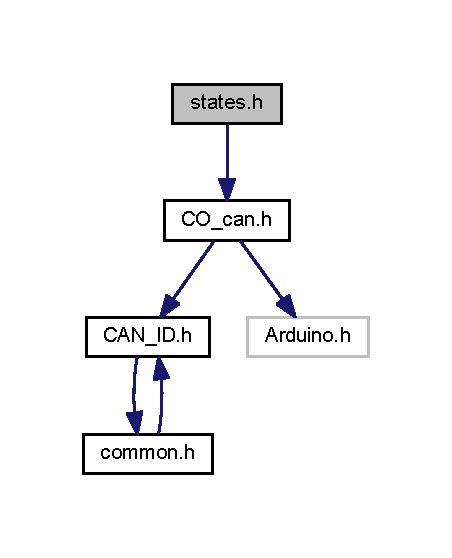
\includegraphics[width=217pt]{states_8h__incl}
\end{center}
\end{figure}
This graph shows which files directly or indirectly include this file\+:\nopagebreak
\begin{figure}[H]
\begin{center}
\leavevmode
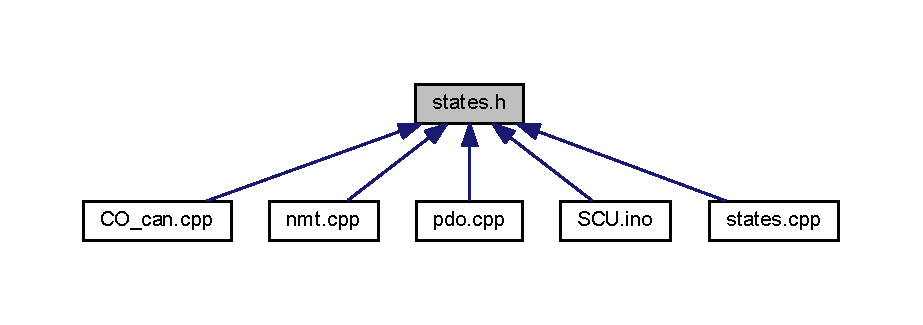
\includegraphics[width=350pt]{states_8h__dep__incl}
\end{center}
\end{figure}
\subsection*{Typedefs}
\begin{DoxyCompactItemize}
\item 
typedef enum \mbox{\hyperlink{group___c_a_nopen___f_s_m__module_ga3136d2815abe9d284f985e0a7ec68646}{enum\+\_\+node\+State}} \mbox{\hyperlink{group___c_a_nopen___f_s_m__module_ga5891f63a4c9243179838389a93d084e2}{e\+\_\+node\+State}}
\end{DoxyCompactItemize}
\subsection*{Enumerations}
\begin{DoxyCompactItemize}
\item 
enum \mbox{\hyperlink{group___c_a_nopen___f_s_m__module_ga3136d2815abe9d284f985e0a7ec68646}{enum\+\_\+node\+State}} \{ \newline
\mbox{\hyperlink{group___c_a_nopen___f_s_m__module_gga3136d2815abe9d284f985e0a7ec68646aeb3ae26d7a1629aa0fc6c83f46306cf5}{Initialisation}} = 0x00, 
\mbox{\hyperlink{group___c_a_nopen___f_s_m__module_gga3136d2815abe9d284f985e0a7ec68646a84ab0fbbb76a8c897feb1cd806d56443}{Disconnected}} = 0x01, 
\mbox{\hyperlink{group___c_a_nopen___f_s_m__module_gga3136d2815abe9d284f985e0a7ec68646a6ea90df6fe966852496b4846da497fb0}{Connecting}} = 0x02, 
\mbox{\hyperlink{group___c_a_nopen___f_s_m__module_gga3136d2815abe9d284f985e0a7ec68646a95fc3c631fbad8ca3dc8d5b69a3e0d5b}{Preparing}} = 0x02, 
\newline
\mbox{\hyperlink{group___c_a_nopen___f_s_m__module_gga3136d2815abe9d284f985e0a7ec68646a4d049c6d45e08a294523df186ad77a75}{Stopped}} = 0x04, 
\mbox{\hyperlink{group___c_a_nopen___f_s_m__module_gga3136d2815abe9d284f985e0a7ec68646aa80594b1522cb686b981f56bbec45124}{Operational}} = 0x05, 
\mbox{\hyperlink{group___c_a_nopen___f_s_m__module_gga3136d2815abe9d284f985e0a7ec68646ac747c16a9c4d7dec65cdab6e38df99b7}{Pre\+\_\+operational}} = 0x7F, 
\mbox{\hyperlink{group___c_a_nopen___f_s_m__module_gga3136d2815abe9d284f985e0a7ec68646acb4b5cb64be091d76f846380eb0afe59}{Unknown\+\_\+state}} = 0x0F
 \}
\end{DoxyCompactItemize}
\subsection*{Functions}
\begin{DoxyCompactItemize}
\item 
void \mbox{\hyperlink{group___c_a_nopen___f_s_m__module_gadfffb3be7aa80aea898ada67e93d2388}{initialisation}} ()
\begin{DoxyCompactList}\small\item\em Initialize \mbox{\hyperlink{group___board__model__group}{Board module}}. If rear S\+CU firmware is selected (according to \mbox{\hyperlink{group___s_c_u__firmware__selection}{S\+CU firmware selection}}) radio is initialized. It initializes the entire application, C\+A\+N/\+C\+A\+Nopen interfaces and communication. \end{DoxyCompactList}\item 
void \mbox{\hyperlink{group___c_a_nopen___f_s_m__module_gaf9e8e3744244bcb2f8b6a8583c0bec0c}{pre\+Operational}} ()
\begin{DoxyCompactList}\small\item\em pre\+Operational state task on the F\+SM. \end{DoxyCompactList}\item 
void \mbox{\hyperlink{group___c_a_nopen___f_s_m__module_ga003b28d176774c489577f471a7b5f946}{operational}} ()
\begin{DoxyCompactList}\small\item\em Start timer for periodic T\+P\+DO transmit according to \mbox{\hyperlink{_c_a_n_network_page}{C\+AN Servizi network}}. \end{DoxyCompactList}\item 
void \mbox{\hyperlink{group___c_a_nopen___f_s_m__module_gad134c6ce7186d3f2e9cb314839fd63ad}{stopped}} ()
\begin{DoxyCompactList}\small\item\em Stop timer for periodic T\+P\+DO transmit according to \mbox{\hyperlink{_c_a_n_network_page}{C\+AN Servizi network}}. \end{DoxyCompactList}\item 
void \mbox{\hyperlink{group___c_a_nopen___f_s_m__module_gabbbb23c086599a8d9432a2121ee82192}{can\+Dispatch}} (\mbox{\hyperlink{struct_message}{Message}} $\ast$m)
\begin{DoxyCompactList}\small\item\em Called by driver when receiving C\+A\+Nopen messages. \end{DoxyCompactList}\item 
\mbox{\hyperlink{group___c_a_nopen___f_s_m__module_ga5891f63a4c9243179838389a93d084e2}{e\+\_\+node\+State}} \mbox{\hyperlink{group___c_a_nopen___f_s_m__module_ga2802a8c3f0174f4e54dd2381968212a0}{get\+State}} ()
\begin{DoxyCompactList}\small\item\em Return current state on the \mbox{\hyperlink{_f_s_m_page}{Finite State Machine (F\+SM)}}. \end{DoxyCompactList}\item 
void \mbox{\hyperlink{group___c_a_nopen___f_s_m__module_ga47cb7615bbcf2c96cc4a7656f9a76bab}{set\+State}} (\mbox{\hyperlink{group___c_a_nopen___f_s_m__module_ga5891f63a4c9243179838389a93d084e2}{e\+\_\+node\+State}} new\+State)
\begin{DoxyCompactList}\small\item\em Set current state on the \mbox{\hyperlink{_f_s_m_page}{Finite State Machine (F\+SM)}}. \end{DoxyCompactList}\end{DoxyCompactItemize}


\subsection{Detailed Description}
C\+A\+Nopen finite state machine header file. 

\begin{DoxyAuthor}{Author}
Arella Matteo ~\newline
 (mail\+: \href{mailto:arella.1646983@studenti.uniroma1.it}{\tt arella.\+1646983@studenti.\+uniroma1.\+it}) 
\end{DoxyAuthor}
\begin{DoxyDate}{Date}
2018 
\end{DoxyDate}

\hypertarget{timer_8cpp}{}\section{timer.\+cpp File Reference}
\label{timer_8cpp}\index{timer.\+cpp@{timer.\+cpp}}


C\+A\+Nopen timer implementation file.  


{\ttfamily \#include $<$Due\+Timer.\+h$>$}\newline
{\ttfamily \#include \char`\"{}common.\+h\char`\"{}}\newline
{\ttfamily \#include \char`\"{}timer.\+h\char`\"{}}\newline
{\ttfamily \#include \char`\"{}pdo.\+h\char`\"{}}\newline
{\ttfamily \#include \char`\"{}C\+O\+\_\+can.\+h\char`\"{}}\newline
{\ttfamily \#include \char`\"{}radio.\+h\char`\"{}}\newline
Include dependency graph for timer.\+cpp\+:\nopagebreak
\begin{figure}[H]
\begin{center}
\leavevmode
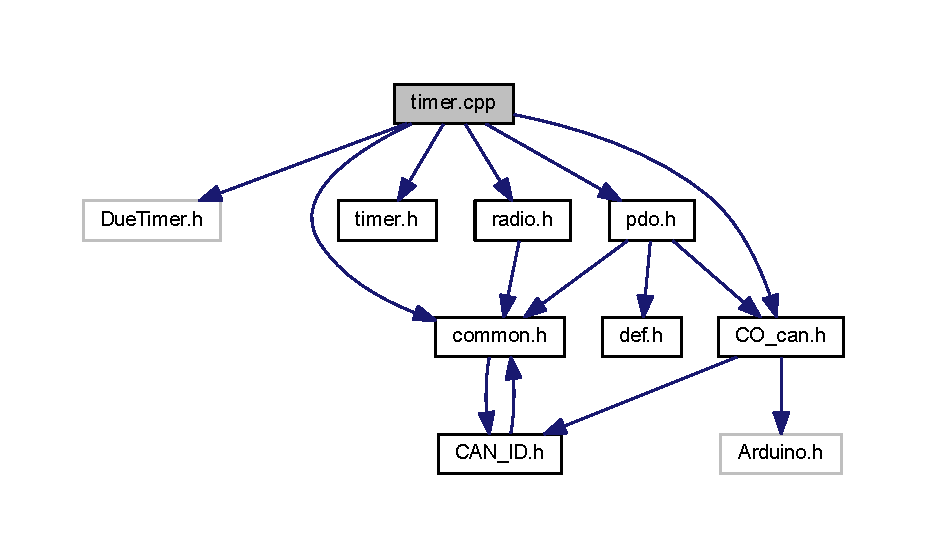
\includegraphics[width=350pt]{timer_8cpp__incl}
\end{center}
\end{figure}
\subsection*{Macros}
\begin{DoxyCompactItemize}
\item 
\#define \mbox{\hyperlink{group___c_a_nopen__timer__module_ga5bb58b675652213c5b20458ab611f9fb}{S\+C\+U\+\_\+\+F\+R\+O\+N\+T\+\_\+\+F\+I\+R\+S\+T\+\_\+\+S\+L\+OT}}~0
\begin{DoxyCompactList}\small\item\em First time slot for $SCU_{Frontal}$. \end{DoxyCompactList}\item 
\#define \mbox{\hyperlink{group___c_a_nopen__timer__module_gae5482bf356c02f4af400a276980e8bbc}{S\+C\+U\+\_\+\+F\+R\+O\+N\+T\+\_\+\+S\+E\+C\+O\+N\+D\+\_\+\+S\+L\+OT}}~1
\begin{DoxyCompactList}\small\item\em Second time slot for $SCU_{Frontal}$. \end{DoxyCompactList}\item 
\#define \mbox{\hyperlink{group___c_a_nopen__timer__module_gaf913e12f6687d34f5ad716d130416dc8}{S\+C\+U\+\_\+\+R\+E\+A\+R\+\_\+\+S\+L\+OT}}~2
\begin{DoxyCompactList}\small\item\em Time slot for $SCU_{Rear}$. \end{DoxyCompactList}\item 
\#define \mbox{\hyperlink{group___c_a_nopen__timer__module_ga266f975ed5b87594263f8a2bf8257cdf}{T\+C\+S\+\_\+\+S\+L\+OT}}~3
\begin{DoxyCompactList}\small\item\em Time slot for $TCU$. \end{DoxyCompactList}\item 
\#define \mbox{\hyperlink{group___c_a_nopen__timer__module_gaab4fadccdeb20ba1f44ed01296b7e560}{T\+I\+M\+E\+\_\+\+S\+L\+O\+T\+\_\+\+M\+A\+SK}}~3
\begin{DoxyCompactList}\small\item\em Time slot mask. \end{DoxyCompactList}\item 
\#define \mbox{\hyperlink{group___c_a_nopen__timer__module_gaf3ebceeca1e0dded3572b4367c5d6413}{R\+A\+D\+I\+O\+\_\+\+S\+L\+O\+T\+\_\+\+M\+A\+SK}}~7
\begin{DoxyCompactList}\small\item\em Radio submit slot mask\+: number of $SCU_{Rear}$ time slots between one submit and successive one (\mbox{\hyperlink{group___common__defines__group_ga09c95853fd002fab968d94c5bc44e823}{T\+I\+M\+E\+\_\+\+S\+L\+O\+T\+\_\+\+P\+E\+R\+I\+OD}} $\ast$ \mbox{\hyperlink{group___c_a_nopen__timer__module_gaf3ebceeca1e0dded3572b4367c5d6413}{R\+A\+D\+I\+O\+\_\+\+S\+L\+O\+T\+\_\+\+M\+A\+SK}} $\ast$ num. time slots between previous and current $SCU_{Rear}$) \end{DoxyCompactList}\end{DoxyCompactItemize}
\subsection*{Functions}
\begin{DoxyCompactItemize}
\item 
void \mbox{\hyperlink{group___c_a_nopen__timer__module_gafa75192a3238525618f8cb83004930cc}{Time\+Dispatch}} ()
\begin{DoxyCompactList}\small\item\em Dispatch time slot for each C\+A\+Nopen node according to \mbox{\hyperlink{_c_a_n_network_page_TPDO_Timer}{T\+P\+D\+O\+\_\+\+Timer}}. \end{DoxyCompactList}\item 
void \mbox{\hyperlink{group___c_a_nopen__timer__module_gaf927959e78504fd1afe1be1e10791ae0}{timer\+Init}} ()
\begin{DoxyCompactList}\small\item\em Initialize timer for periodic submit of T\+P\+D\+Os. \end{DoxyCompactList}\item 
void \mbox{\hyperlink{group___c_a_nopen__timer__module_gaddf92f4b7b741f7b9fbc827d2e4f2a8b}{timer\+Start}} ()
\begin{DoxyCompactList}\small\item\em Start timer for periodic submit of T\+P\+D\+Os. \end{DoxyCompactList}\item 
void \mbox{\hyperlink{group___c_a_nopen__timer__module_gaecc39b6c4a6a4d79a46ac2b6371221c5}{timer\+Stop}} ()
\begin{DoxyCompactList}\small\item\em Stop timer for periodic submit of T\+P\+D\+Os. \end{DoxyCompactList}\end{DoxyCompactItemize}
\subsection*{Variables}
\begin{DoxyCompactItemize}
\item 
volatile uint8\+\_\+t \mbox{\hyperlink{group___c_a_nopen__timer__module_ga38a43dbb3c9d41a62672688eb57fa33f}{t\+\_\+slot}} = \mbox{\hyperlink{group___c_a_nopen__timer__module_ga5bb58b675652213c5b20458ab611f9fb}{S\+C\+U\+\_\+\+F\+R\+O\+N\+T\+\_\+\+F\+I\+R\+S\+T\+\_\+\+S\+L\+OT}}
\begin{DoxyCompactList}\small\item\em Current time slot. \end{DoxyCompactList}\item 
volatile uint8\+\_\+t \mbox{\hyperlink{group___c_a_nopen__timer__module_gac230d484e56093c9ba05a68a6f954ae6}{radio\+\_\+slot}} = 0
\begin{DoxyCompactList}\small\item\em Current radio time slot. \end{DoxyCompactList}\item 
Due\+Timer $\ast$ \mbox{\hyperlink{group___c_a_nopen__timer__module_ga76a145cc4b1fbdcbf86505111dfc6b21}{timer}}
\begin{DoxyCompactList}\small\item\em Timer for periodic T\+P\+DO submit. \end{DoxyCompactList}\end{DoxyCompactItemize}


\subsection{Detailed Description}
C\+A\+Nopen timer implementation file. 

\begin{DoxyAuthor}{Author}
Arella Matteo ~\newline
 (mail\+: \href{mailto:arella.1646983@studenti.uniroma1.it}{\tt arella.\+1646983@studenti.\+uniroma1.\+it}) 
\end{DoxyAuthor}
\begin{DoxyDate}{Date}
2018 
\end{DoxyDate}

\hypertarget{timer_8h}{}\section{timer.\+h File Reference}
\label{timer_8h}\index{timer.\+h@{timer.\+h}}


C\+A\+Nopen timer header file.  


This graph shows which files directly or indirectly include this file\+:\nopagebreak
\begin{figure}[H]
\begin{center}
\leavevmode
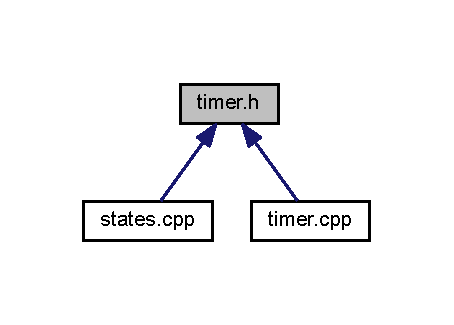
\includegraphics[width=218pt]{timer_8h__dep__incl}
\end{center}
\end{figure}
\subsection*{Functions}
\begin{DoxyCompactItemize}
\item 
void \mbox{\hyperlink{group___c_a_nopen__timer__module_gaf927959e78504fd1afe1be1e10791ae0}{timer\+Init}} ()
\begin{DoxyCompactList}\small\item\em Initialize timer for periodic submit of T\+P\+D\+Os. \end{DoxyCompactList}\item 
void \mbox{\hyperlink{group___c_a_nopen__timer__module_gaddf92f4b7b741f7b9fbc827d2e4f2a8b}{timer\+Start}} ()
\begin{DoxyCompactList}\small\item\em Start timer for periodic submit of T\+P\+D\+Os. \end{DoxyCompactList}\item 
void \mbox{\hyperlink{group___c_a_nopen__timer__module_gaecc39b6c4a6a4d79a46ac2b6371221c5}{timer\+Stop}} ()
\begin{DoxyCompactList}\small\item\em Stop timer for periodic submit of T\+P\+D\+Os. \end{DoxyCompactList}\item 
void \mbox{\hyperlink{group___c_a_nopen__timer__module_gafa75192a3238525618f8cb83004930cc}{Time\+Dispatch}} ()
\begin{DoxyCompactList}\small\item\em Dispatch time slot for each C\+A\+Nopen node according to \mbox{\hyperlink{_c_a_n_network_page_TPDO_Timer}{T\+P\+D\+O\+\_\+\+Timer}}. \end{DoxyCompactList}\end{DoxyCompactItemize}


\subsection{Detailed Description}
C\+A\+Nopen timer header file. 

\begin{DoxyAuthor}{Author}
Arella Matteo ~\newline
 (mail\+: \href{mailto:arella.1646983@studenti.uniroma1.it}{\tt arella.\+1646983@studenti.\+uniroma1.\+it}) 
\end{DoxyAuthor}
\begin{DoxyDate}{Date}
2018 
\end{DoxyDate}

%--- End generated contents ---

% Index
\backmatter
\newpage
\phantomsection
\clearemptydoublepage
\addcontentsline{toc}{chapter}{Index}
\printindex

\end{document}
